\mfpicnumber{1}
\opengraphsfile{IntroRational}

\setcounter{footnote}{0}

\label{IntroRational}


If we add, subtract, or multiply polynomial functions, the result is another polynomial function.  When we divide polynomial functions, however, we may not get a polynomial function.   The result of dividing two polynomials is a   \index{rational function} \textbf{rational function}, so named because rational functions  are \textbf{ratios} of polynomials.

\smallskip

\colorbox{ResultColor}{\bbm

\begin{defn}  \label{rationalfunction} A \textbf{rational function} is a function which is the ratio of polynomial functions.  Said differently, $r$ is a rational function if it is of the form \index{function ! rational}

\[ r(x) = \dfrac{p(x)}{q(x)},\]

where $p$ and $q$ are polynomial functions.\footnote{According to this definition, all polynomial functions are also  rational functions. (Take $q(x) = 1$).}

\end{defn}

\ebm}

\subsection{Laurent Monomial Functions}
\label{LaurentMonomialFunctionsSection}

As with polynomial functions, we begin our study of rational functions with what are, in some sense, the building blocks of rational functions, \index{monomial function ! Laurent}\index{function ! monomial ! Laurent}\textbf{Laurent monomial functions}.  

\colorbox{ResultColor}{\bbm

\begin{defn}  \label{laurentmonomialfunction} A \textbf{Laurent monomial function} is either a monomial function (see Definition \ref{monomialfunction}) or a function of the form $f(x) = \dfrac{a}{x^n} = ax^{-n}$ for $n \in \mathbb{N}$.

\end{defn}

\ebm}

Laurent monomial functions are named in honor of \href{https://en.wikipedia.org/wiki/Pierre_Alphonse_Laurent}{\underline{Pierre Alphonse Laurent}} and generalize the notion of `monomial function' from Chapter \ref{PolynomialFunctions} to terms with negative exponents. Our study of these functions begins with an analysis of   $r(x) = \frac{1}{x} = x^{-1}$, the reciprocal function. The first item worth  noting is that $r(0)$ is not defined owing to the presence of $x$  in the denominator.  That is, the domain of $r$ is $\{ x \in \mathbb{R} \, | \, x \neq 0\}$ or, using interval notation, $(-\infty, 0) \cup (0, \infty)$.   Of course excluding $0$ from the domain of $r$ serves only to pique our curiosity about the behavior of $r(x)$ when $x \approx 0$.  Thinking from a number sense perspective, the closer the denominator of $\frac{1}{x}$ is to $0$, the larger the value of the  fraction (in absolute value.)\footnote{Technically speaking, $-1 \times 10^{117}$ is a `small' number (since it is very far to the left on the number line.)  However, it's absolute value, $1 \times 10^{117}$ is very large.  If you read footnotes, you've seen this clarification before \ldots (see Section \ref{GraphsofPolynomials}.)}  So it stands to reason that as $x$ gets closer and closer to $0$, the values for $r(x) = \frac{1}{x}$ should grow larger and larger (in absolute value.)  This is borne out in the table below on the left where it is apparent that for $x \approx 0$, $r(x)$ is becoming unbounded.



As we investigate the end behavior of $r$, we find that as $x \rightarrow -\infty$ and as $x \rightarrow \infty$, $r(x) \approx 0$. Again, number sense agrees here with the data, since as the denominator of $\frac{1}{x}$ becomes unbounded, the value of the fraction should diminish.\footnote{We'll talk more about this end behavior shortly - stay tuned!} That being said, we could ask if the graph ever reaches the $x$-axis.  If we attempt to solve $y = r(x) = \frac{1}{x} = 0$. we arrive at the contradiction $1 = 0$ hence, $0$ is not in the range of $r$.  Every other real number besides $0$ is in the range of $r$, however.  To see this, let $c \neq 0$ be a real number.  Then $\frac{1}{c}$ is defined and, moreover, $r \left(\frac{1}{c} \right) = \frac{1}{(1/c)} = c$.  This shows $c$ is in the range of $r$.  Hence, the range of $r$ is $\{ y \in \mathbb{R} \, | \, y \neq 0\}$ or, using interval notation,  $(-\infty, 0) \cup (0, \infty)$.  

\begin{center}
\begin{tabular}{m{2in}m{2in}m{2in}}

$\begin{array}{|r||c|}  \hline

  x & r(x) = \frac{1}{x}  \\ \hline
 -0.01& -100  \\  \hline
 -0.001 & -1000  \\  \hline 
 -0.0001 & -10000  \\  \hline 
 -0.00001 & -100000 \\  \hline 
0 & \text{undefined} \\  \hline
0.00001 & 100000 \\  \hline  
0.0001 & 10000  \\  \hline 
 0.001 & 1000  \\  \hline 
 0.01 & 100  \\  \hline
  \end{array} $
  
  &
  
  $\begin{array}{|r||c|}  \hline

  x & r(x) = \frac{1}{x}  \\ \hline
 -100000 & -0.00001  \\  \hline 
 -10000 &  -0.0001 \\  \hline 
 -1000 & -0.001  \\  \hline 
 -100 & -0.01  \\  \hline
0 & \text{undefined} \\  \hline
 100 & 0.01  \\  \hline
 1000 & 0.001  \\  \hline 
 10000 & 0.0001 \\  \hline
 100000 & 0.00001  \\  \hline  
  \end{array} $
  
  &
  
\begin{mfpic}[15]{-5}{5}{-5}{5}
\axes
\scriptsize
\tlabel[cc](5, -0.5){$x$}
\tlabel[cc](0.5, 5){$y$}
\tlabel[cc](-2, -1.5){$(-1,-1)$}
\tlabel[cc](2, 1.5){$(1,1)$}
\normalsize
\penwd{1.25pt}
\arrow \reverse \arrow \function{-5,-0.2,0.1}{1/x}
\arrow \reverse \arrow \function{0.2,5,0.1}{1/x}
\point[4pt]{(-1,-1), (1,1)}
\tcaption{\scriptsize $y=r(x) = \frac{1}{x}$}
\end{mfpic}\\



\end{tabular}

\end{center}

Like we did in Section \ref{GraphsofPolynomials}, we'll borrow some notation from Calculus in order for us to codify the behavior as $x \rightarrow 0$.  First off, note that the behavior of $r$ differs depending on which direction we approach $0$.  We describe the values $x<0$ but $x \rightarrow 0$  (such as $x = -0.01$, $-0.001$, etc.)  as  `$x$ approaching $0$ \textbf{from the left},' written as $x \rightarrow 0^{-}$.  If we think of these numbers as all being $x$-values where  $x  = \text{`$0-$ a little bit'}$, the  the `$-$' in the notation `$x \rightarrow 0^{-}$' makes better sense.  For these values,  the function values $r(x) \rightarrow -\infty$.   Using the limit notation introduced in Section \ref{GraphsofPolynomials}, we'd write: $\ds{ \lim_{x \rightarrow 0^{-}} r(x) = - \infty}$.  


Similarly, we say `as $x$ approaches $0$ \textbf{from the right},' that is as $x \rightarrow 0^{+}$, $r(x) \rightarrow \infty$, or, more succinctly, $\ds{ \lim_{x \rightarrow 0^{+}} r(x) =  \infty}$.  As before, we understand `from the right' means we are using $x$ values slightly to the \textbf{right} of $0$ on the number line:  numbers such as $x =0.001.$ These numbers could described as `$0 + \text{a little bit}$,' which justifies the `$+$' in the notation `$x \rightarrow 0^{+}$.'

We can also use this notation to describe the end behavior, but here the numerical roles are reversed.  We see as $x \rightarrow -\infty$, $r(x) \rightarrow 0^{-}$ and as $x \rightarrow \infty$, $r(x) \rightarrow 0^{+}$.  When it comes to codifying these results using Calculus, we write $\ds{ \lim_{x \rightarrow -\infty} r(x) =  0}$ and $\ds{ \lim_{x \rightarrow \infty} r(x) =  0}$.  Note that, unfortunately, we lose the directionality here on the limiting value - that is, we do not write $\ds{ \lim_{x \rightarrow -\infty} r(x) =  0^{-}}$ or $\ds{ \lim_{x \rightarrow \infty} r(x) =  0^{+}}$.  Without getting too much into formal definitions, the reason is that if limiting values are finite, we express them as real numbers.\footnote{We will, of course, offer more detail if the situation presents itself.}  Period.

The way we describe what is happening graphically is to say the line $x = 0$ is a  \index{asymptote ! vertical ! intuitive definition of}\index{vertical asymptote ! intuitive definition of}\textbf{vertical asymptote}  to the graph of $y = r(x)$ and the line $y = 0$ is a \index{asymptote ! horizontal ! intuitive definition of}\index{horizontal asymptote ! intuitive definition of}\textbf{horizontal asymptote} to the graph of $y = r(x)$.  Roughly speaking, asymptotes are lines which approximate functions as either the inputs or outputs become unbounded. 

\colorbox{ResultColor}{\bbm

\begin{defn} \label{va} The line $x=c$ is called a \index{asymptote ! vertical ! formal definition of}\index{vertical asymptote ! formal definition of}\textbf{vertical asymptote} of the graph of a function $y=f(x)$  if either of the limits $\ds{ \lim_{x \rightarrow c^{-}} f(x)}$ or  $\ds{ \lim_{x \rightarrow c^{+}} f(x)}$ (or both) result in $\infty$ or $-\infty$.

\end{defn}
\ebm}

\medskip


\colorbox{ResultColor}{\bbm

\begin{defn} \label{ha} The line $y=c$ is called a \index{asymptote ! horizontal ! formal definition of}\index{horizontal asymptote ! formal definition of}\textbf{horizontal asymptote} of the graph of a function $y=f(x)$ either  $\ds{ \lim_{x \rightarrow -\infty} f(x)=c}$ or  $\ds{ \lim_{x \rightarrow \infty} f(x)=c}$ (or both).
\end{defn}
\ebm}

\medskip


The behaviors illustrated in the graph $r(x) = \frac{1}{x}$ are typical of functions of the form $f(x) = \frac{1}{x^n} = x^{-n}$ for natural numbers, $n$.  As with the monomial functions discussed in Section \ref{GraphsofPolynomials}, the patterns that develop primarily depend on whether $n$ is odd or even.  Having thoroughly discussed the graph of $y = \frac{1}{x} = x^{-1}$, we graph it along with $y = \frac{1}{x^3} = x^{-3}$ and $y = \frac{1}{x^5} = x^{-5}$ below.  Note the points $(-1,-1)$ and $(1,1)$ are common to all three graphs as are the asymptotes $x = 0$ and $y = 0$.  As the $n$ increases, the graphs become steeper for $|x| < 1$  and flatten out more quickly for $|x|>1$.  Both the domain and range in each case appears to be $(-\infty, 0) \cup (0, \infty)$.  Indeed, owing to the $x$ in the denominator of $f(x) = \frac{1}{x^n}$, $f(0)$, and only $f(0)$,  is undefined. Hence the domain is $(-\infty, 0) \cup (0, \infty)$.  When thinking about the range, note the equation  $f(x)= \frac{1}{x^n}  = c$ has the solution $x = \sqrt[n]{\frac{1}{c}}$ as long as $c \neq 0$.  Thus means $f\left( \sqrt[n]{\frac{1}{c}} \right) = c$ for every nonzero real number $c$.  If $c = 0$, we are in the same situation as before:  $\frac{1}{x^n} = 0$ has no real solution.  This establishes the range is $(-\infty, 0) \cup (0, \infty)$.  Finally, each of the graphs appear to be symmetric about the origin.  Indeed, since $n$ is odd, $f(-x) = (-x)^{-n} = (-1)^{-n} x^{-n} = -x^{-n} = -f(x)$, proving every member of this function family is odd.  

\begin{tabular}{m{2.75in}m{1.25in}m{1.25in}m{1.25in}}

$\begin{array}{|r||c|c|c|}  \hline

 x &  \frac{1}{x} = x^{-1} & \frac{1}{x^3} = x^{-3} & \frac{1}{x^5} = x^{-5} \\ \hline
 -10 & -0.1 &-0.001& -0.00001  \\  \hline
 -1 & -1 & -1&  -1\\  \hline
 -0.1 & -10 & -1000&  -100000 \\  \hline
 0 &  \text{undefined} &  \text{undefined}  &  \text{undefined}  \\  \hline
 0.1 & 10 & 1000&  100000 \\  \hline
 1 & 1 & 1&  1\\  \hline
 10 & 0.1 & 0.001& 0.00001  \\  \hline

\end{array}$

&

\begin{mfpic}[9]{-5}{5}{-5}{5}
\axes
\scriptsize
\tlabel[cc](5, -0.5){$x$}
\tlabel[cc](-0.5, 5){$y$}
\normalsize
\penwd{1.25pt}
\arrow \reverse \arrow \function{-5,-0.2,0.1}{1/x}
\arrow \reverse \arrow \function{0.2,5,0.1}{1/x}
\point[4pt]{(-1,-1), (1,1)}
\tcaption{\scriptsize $y=\frac{1}{x} = x^{-1}$}
\end{mfpic}

&

\begin{mfpic}[9]{-5}{5}{-5}{5}
\axes
\scriptsize
\tlabel[cc](5, -0.5){$x$}
\tlabel[cc](-0.5, 5){$y$}
\normalsize
\penwd{1.25pt}
\arrow \reverse \arrow \function{-5,-0.58,0.1}{1/(x**3)}
\arrow \reverse \arrow \function{0.58,5,0.1}{1/(x**3)}
\point[4pt]{(-1,-1),  (1,1)}
\tcaption{\scriptsize $y=\frac{1}{x^3} = x^{-3}$}
\end{mfpic}

&

\begin{mfpic}[9]{-5}{5}{-5}{5}
\axes
\scriptsize
\tlabel[cc](5, -0.5){$x$}
\tlabel[cc](-0.5, 5){$y$}
\normalsize
\penwd{1.25pt}
\arrow \reverse \arrow \function{-5,-0.72,0.1}{1/(x**5)}
\arrow \reverse \arrow \function{0.725,5,0.1}{1/(x**5)}
\point[4pt]{(-1,-1), (1,1)}
\tcaption{\scriptsize $y=\frac{1}{x^5} = x^{-5}$}
\end{mfpic} \\

\end{tabular}

We repeat the same experiment with functions of the form $f(x) = \frac{1}{x^{n}} = x^{-n}$ where $n$ is even. $y = \frac{1}{x^2} = x^{-2}$, $y = \frac{1}{x^4} = x^{-4}$ and $y = \frac{1}{x^6} = x^{-6}$.  These graphs all share the points $(-1,1)$ and $(1,1)$, and asymptotes $x = 0$ and $y = 0$.  Note here that both $\ds{\lim_{x \rightarrow 0^{-}} f(x) = \infty}$ and $\ds{\lim_{x \rightarrow 0^{+}} f(x) = \infty}$, so we may simply write $\ds{\lim_{x \rightarrow 0} f(x) = \infty}$. 

The same remarks about the steepness for $|x|<1$ and the flattening for $|x|>1$ also apply. For the same reasons as given above, the domain of each of these functions is $(-\infty, 0) \cup (0, \infty)$.  When it comes to the range, the fact $n$ is even tells us there are  solutions to $\frac{1}{x^n} = c$ only if $c>0$. It follows that the range is $(0, \infty)$ for each of these functions.  Concerning symmetry, as $n$ is even, $f(-x) = (-x)^{-n} = (-1)^{-n} x^{-n} = x^{-n} = f(x)$, proving each member of this function family is even.  Hence,  the graphs of these functions are symmetric about the $y$-axis.


\begin{tabular}{m{2.75in}m{1.25in}m{1.25in}m{1.25in}}

$\begin{array}{|r||c|c|c|}  \hline

 x &  \frac{1}{x^2} = x^{-2} & \frac{1}{x^4} = x^{-4} & \frac{1}{x^6} = x^{-6} \\ \hline
 -10 &0.01 &0.0001& 1 \times 10^{-6}  \\  \hline
 -1 & 1 & 1&  1\\  \hline
 -0.1 & 100 & 10000 &  1 \times 10^{6} \\  \hline
 0 &  \text{undefined} &  \text{undefined}  &  \text{undefined}  \\  \hline
0.1 & 100 & 10000 &  1 \times 10^{6} \\  \hline
 1&  1 & 1&  1 \\  \hline
10 &0.01 &0.0001& 1 \times 10^{-6}  \\  \hline

\end{array}$

&

\begin{mfpic}[9]{-5}{5}{-1}{9}
\axes
\scriptsize
\tlabel[cc](5, -0.5){$x$}
\tlabel[cc](0, 9.5){$y$}
\normalsize
\penwd{1.25pt}
\arrow \reverse \arrow \function{-5,-0.3333,0.1}{1/(x**2)}
\arrow \reverse \arrow \function{0.3333,5,0.1}{1/(x**2)}
\point[4pt]{(-1,1), (1,1)}
\tcaption{\scriptsize $y=\frac{1}{x^2} = x^{-2}$}
\end{mfpic}

&

\begin{mfpic}[9]{-5}{5}{-1}{9}
\axes
\scriptsize
\tlabel[cc](5, -0.5){$x$}
\tlabel[cc](0, 9.5){$y$}
\normalsize
\penwd{1.25pt}
\arrow \reverse \arrow \function{-5,-0.5774,0.1}{1/(x**4)}
\arrow \reverse \arrow \function{0.5773,5,0.1}{1/(x**4)}
\point[4pt]{(-1,1), (1,1)}
\tcaption{\scriptsize $y=\frac{1}{x^3} = x^{-3}$}
\end{mfpic}

&

\begin{mfpic}[9]{-5}{5}{-1}{9}
\axes
\scriptsize
\tlabel[cc](5, -0.5){$x$}
\tlabel[cc](0, 9.5){$y$}
\normalsize
\penwd{1.25pt}
\arrow \reverse \arrow \function{-5,-0.6933,0.1}{1/(x**6)}
\arrow \reverse \arrow \function{0.6933,5,0.1}{1/(x**6)}
\point[4pt]{(-1,1), (1,1)}
\tcaption{\scriptsize $y=\frac{1}{x^6} = x^{-6}$}
\end{mfpic} \\

\end{tabular}


Not surprisingly, we have an analog to Theorem \ref{linearmononialgraphs} for this family of Laurent monomial functions.

\colorbox{ResultColor}{\bbm

\begin{thm} \label{linearlaurentlgraphs}  For real numbers $a$, $h$, and $k$ with $a \neq 0$, the graph of $F(x) = \frac{a}{(x-h)^n}+k =  a(x-h)^{-n}+k$  can be obtained from the graph of $f(x) = \frac{1}{x^n}= x^{-n}$ by performing the following operations, in sequence:

\begin{enumerate}

\item  add $h$ to each of the $x$-coordinates of the points on the graph of $f$.  This results in a horizontal shift to the right if $h > 0$ or left if $h < 0$.

\textbf{NOTE:}  This transforms the graph of $y = x^{-n}$ to $y = (x-h)^{-n}$.   

The vertical asymptote moves from $x=0$ to $x=h$.

\item  multiply the $y$-coordinates of the points on the graph obtained in Step 1 by $a$.   This results in a vertical scaling, but may also include a reflection about the $x$-axis if $a < 0$.

\textbf{NOTE:}  This transforms the graph of $y = (x-h)^{-n}$ to $y = a(x-h)^{-n}$.

\item  add $k$ to each of the $y$-coordinates of the points on the graph obtained in Step 2.  This results in a vertical shift up if $k > 0$ or down if $k< 0$.

\textbf{NOTE:}  This transforms the graph of  $y = a(x-h)^{-n}$ to $y = a(x-h)^{-n}+k$.

The  horizontal asymptote moves from $y=0$ to $y=k$.

\end{enumerate}

\end{thm}

\ebm}


The proof of Theorem \ref{linearlaurentlgraphs} is \textbf{identical} to the proof of Theorem \ref{linearmononialgraphs} - just replace $x^n$ with $x^{-n}$.  We nevertheless encourage the reader to work through the details\footnote{We are, in fact, building to Theorem \ref{transformationsthm} in Section \ref{Transformations}, so the more you see the forest for the trees, the better off you'll be when the time comes to generalize these moves to all functions.} and compare the results of this theorem with Theorems \ref{linearabsvaluegraphs}, \ref{standardformgraph}, and  \ref{linearmononialgraphs}.


We put Theorem \ref{linearlaurentlgraphs} to good use in the following example.

\begin{ex} \label{linearlaurentex} Use Theorem \ref{linearlaurentlgraphs} to graph the following.  Label at least two points and the asymptotes.  State the domain and range using interval notation.


\begin{enumerate}

\begin{multicols}{2}

\item  $f(x) = (2x-3)^{-2}$ \vphantom{$g(t) = \dfrac{2t-1}{t+1}$}

\item  $g(t) = \dfrac{2t-1}{t+1}$

\end{multicols}

\end{enumerate}

{\bf Solution.} 

\begin{enumerate}

\item In order to use Theorem \ref{linearlaurentlgraphs}, we first must put $f(x) = (2x-3)^{-2}$ into the form prescribed by the theorem.  To that end, we factor:  \[f(x) = \left(2 \left[x  - \frac{3}{2} \right] \right)^{-2} = 2^{-2} \left(x - \frac{3}{2} \right)^{-2} = \frac{1}{4}  \left(x - \frac{3}{2} \right)^{-2}\]

We identify $n=2$, $a=\frac{1}{4}$ and $h = \frac{3}{2}$ (and $k =0$.)  Per the theorem, we begin with the graph of $y = x^{-2}$ and track the two points $(-1,1)$ and $(1,1)$ along with the vertical and horizontal asymptotes $x = 0$ and $y=0$, respectively through each step.

Step 1:   add $\frac{3}{2}$ to each of the $x$-coordinates of each of the points on the graph of $y=x^{-2}$.  This moves the vertical asymptote from $x = 0$ to $x = \frac{3}{2}$ (which we represent by a dashed line.)

\[ \begin{array}{ccc}


\begin{mfpic}[15]{-5}{5}{-1}{9}
\axes
\scriptsize
\tlabel[cc](5, -0.5){$x$}
\tlabel[cc](0, 9.5){$y$}
\tlabel[cc](-2, 1){$(-1,1)$}
\tlabel[cc](2, 1){$(1,1)$}
\normalsize
\penwd{1.25pt}
\arrow \reverse \arrow \function{-5,-0.3333,0.1}{1/(x**2)}
\arrow \reverse \arrow \function{0.3333,5,0.1}{1/(x**2)}
\point[4pt]{(-1,1), (1,1)}
\tcaption{\scriptsize $y = x^{-2}$}
\end{mfpic}


&
\stackrel{\text{ \scriptsize add $\frac{3}{2}$ to each $x$-coordinate}}{\xrightarrow{\hspace{1.5in}}}
&

\begin{mfpic}[15]{-3.5}{6.5}{-1}{9}
\axes
\dashed \polyline{(1.5, -1), (1.5,9)}
\scriptsize
\tlabel[cc](6.5, -0.5){$x$}
\tlabel[cc](0.5, 9){$y$}
\gclear \tlabelrect[cc](-0.5, 1){$\left(\frac{1}{2} ,1 \right)$}
\tlabel[cc](3.5, 1){$\left(\frac{5}{2} ,1 \right)$}
\gclear \tlabelrect[cc](1.5, -0.5){$x = \frac{3}{2}$}
\normalsize
\penwd{1.25pt}
\arrow \reverse \arrow \function{-3.5,1.1667,0.1}{1/((x-1.5)**2)}
\arrow \reverse \arrow \function{1.8333,6.5,0.1}{1/((x-1.5)**2)}
\point[4pt]{(0.5,1), (2.5,1)}
\tcaption{\scriptsize $y = \left(x - \frac{3}{2} \right)^{-2}$}
\end{mfpic} \\

 \text{\scriptsize  $(-1,1)$, VA: $x=0$ , $(1,1)$} & & \text{\scriptsize  $\left(\frac{1}{2} ,1 \right)$, VA: $x = \frac{3}{2}$,  $\left(\frac{5}{2} ,1 \right)$} \\
 
 \end{array} \]

Step 2:   multiply each of the $y$-coordinates of each of the points on the graph of $y = \left(x - \frac{3}{2} \right)^{-2}$ by $\frac{1}{4}$. 
 \[ \begin{array}{ccc}
 
\begin{mfpic}[15]{-3.5}{6.5}{-1}{9}
\axes
\dashed \polyline{(1.5, -1), (1.5,9)}
\scriptsize
\tlabel[cc](6.5, -0.5){$x$}
\tlabel[cc](0.5, 9){$y$}
\gclear \tlabelrect[cc](-0.5, 1){$\left(\frac{1}{2} ,1 \right)$}
\tlabel[cc](3.5, 1){$\left(\frac{5}{2} ,1 \right)$}
\gclear \tlabelrect[cc](1.5, -0.5){$x = \frac{3}{2}$}
\normalsize
\penwd{1.25pt}
\arrow \reverse \arrow \function{-3.5,1.1667,0.1}{1/((x-1.5)**2)}
\arrow \reverse \arrow \function{1.8333,6.5,0.1}{1/((x-1.5)**2)}
\point[4pt]{(0.5,1), (2.5,1)}
\tcaption{\scriptsize $y = \left(x - \frac{3}{2} \right)^{-2}$}
\end{mfpic} 

&

\stackrel{\text{ \scriptsize multiply each $y$-coordinate by $\frac{1}{4}$ }}{ \xrightarrow{\hspace{1.5in}}}

&

\begin{mfpic}[15]{-3.5}{6.5}{-1}{9}
\axes
\dashed \polyline{(1.5, -1), (1.5,9)}
\scriptsize
\tlabel[cc](6.5, -0.5){$x$}
\tlabel[cc](0.5, 9){$y$}
\gclear \tlabelrect[cc](-0.5, 0.5){$\left(\frac{1}{2} ,\frac{1}{4} \right)$}
\tlabel[cc](3.5, 0.5){$\left(\frac{5}{2} ,\frac{1}{4} \right)$}
\gclear \tlabelrect[cc](1.5, -0.5){$x = \frac{3}{2}$}
\normalsize
\penwd{1.25pt}
\arrow \reverse \arrow \function{-3.5,1.3333,0.1}{0.25/((x-1.5)**2)}
\arrow \reverse \arrow \function{1.6667,6.5,0.1}{0.25/((x-1.5)**2)}
\point[4pt]{(0.5,0.25), (2.5,0.25)}
\tcaption{\scriptsize $y = \frac{1}{4} \left(x - \frac{3}{2} \right)^{-2}$}
\end{mfpic} \\


\text{\scriptsize  $\left(\frac{1}{2} ,1 \right)$,  $\left(\frac{5}{2} ,1 \right)$} & &\text{\scriptsize  $\left(\frac{1}{2} ,\frac{1}{4} \right)$,  $\left(\frac{5}{2} , \frac{1}{4} \right)$}  \\ \end{array} \]


Since we did not shift the graph vertically, the horizontal asymptote remains $y = 0$.  We can determine the domain and range of $f$ by tracking the changes to the domain and range of our progenitor function, $y = x^{-2}$.  We get the domain and range of $f$ is  $\left(-\infty, \frac{3}{2} \right) \cup \left(\frac{3}{2}, \infty \right)$ and the range of $f$ is $(-\infty, 0) \cup (0, \infty)$. 

\item  Using either long or synthetic division, we get \[g(t) = \frac{2t-1}{t+1} = - \frac{3}{t+1} + 2 = \frac{-3}{(t-(-1))^{1}} + 2\] so we identify $n = 1$, $a = -3$, $h = -1$, and $k = 2$.  We start with the graph of $y = \frac{1}{t}$ with points $(-1,-1)$, $(1,1)$ and asymptotes $t = 0$ and $y =0$ and track these through each of the steps.

Step 1:  Add $-1$ to each of the $t$-coordinates of each of the points on the graph of $y = \frac{1}{t}$. This moves the vertical asymptote from $t=0$ to $t = -1$. 

\[ \begin{array}{ccc}


\begin{mfpic}[15]{-5}{5}{-5}{5}
\axes
\scriptsize
\tlabel[cc](5, -0.5){$t$}
\tlabel[cc](0.5, 5){$y$}
\tlabel[cc](-2, -1.5){$(-1,-1)$}
\tlabel[cc](2, 1.5){$(1,1)$}
\normalsize
\penwd{1.25pt}
\arrow \reverse \arrow \function{-5,-0.2,0.1}{1/x}
\arrow \reverse \arrow \function{0.2,5,0.1}{1/x}
\point[4pt]{(-1,-1), (1,1)}
\tcaption{\scriptsize $y = \frac{1}{t}$}
\end{mfpic}



&
\stackrel{\text{ \scriptsize add $-1$ to each $t$-coordinate}}{\xrightarrow{\hspace{1.5in}}}
&

\begin{mfpic}[15]{-6}{4}{-5}{5}
\axes
\dashed \polyline{(-1,-5), (-1,5)}
\scriptsize
\tlabel[cc](4, -0.5){$t$}
\tlabel[cc](0.5, 5){$y$}
\tlabel[cc](-3, -1.5){$(-2,-1)$}
\tlabel[cc](1, 1.5){$(0,1)$}
\tlabel[cc](-2, 4){$t= -1$}
\normalsize
\penwd{1.25pt}
\arrow \reverse \arrow \function{-6,-1.2,0.1}{1/(x+1)}
\arrow \reverse \arrow \function{-0.8,4,0.1}{1/(x+1)}
\point[4pt]{(-2,-1), (0,1)}
\tcaption{\scriptsize $y= \frac{1}{t+1}$}
\end{mfpic} \\

 \text{\scriptsize  $(-1,1)$, VA: $t=0$ , $(1,1)$} & & \text{\scriptsize   $(-2,1)$, VA: $t=-1$ , $(0,1)$} \\
 
 \end{array} \]

Step 2:   multiply each of the $y$-coordinates of each of the points on the graph of $y = \frac{1}{t+1}$ by $-3$. 

\[ \begin{array}{ccc}


\begin{mfpic}[15]{-6}{4}{-5}{5}
\axes
\dashed \polyline{(-1,-5), (-1,5)}
\scriptsize
\tlabel[cc](4, -0.5){$t$}
\tlabel[cc](0.5, 5){$y$}
\tlabel[cc](-3, -1.5){$(-2,-1)$}
\tlabel[cc](1, 1.5){$(0,1)$}
\tlabel[cc](-2, 4){$t= -1$}
\normalsize
\penwd{1.25pt}
\arrow \reverse \arrow \function{-6,-1.2,0.1}{1/(x+1)}
\arrow \reverse \arrow \function{-0.8,4,0.1}{1/(x+1)}
\point[4pt]{(-2,-1), (0,1)}
\tcaption{\scriptsize $y= \frac{1}{t+1}$}
\end{mfpic} 



&
\stackrel{\text{ \scriptsize multiply each $y$-coordinate by $-3$}}{\xrightarrow{\hspace{1.5in}}}
&

\begin{mfpic}[15]{-6}{4}{-5}{5}
\axes
\dashed \polyline{(-1,-5), (-1,5)}
\scriptsize
\tlabel[cc](4, -0.5){$t$}
\tlabel[cc](0.5, 5){$y$}
\tlabel[cc](-3, 3){$(-2,3)$}
\tlabel[cc](1, -3){$(0,-3)$}
\tlabel[cc](-2, -4){$t= -1$}
\normalsize
\penwd{1.25pt}
\arrow \reverse \arrow \function{-6,-1.6,0.1}{0-3/(x+1)}
\arrow \reverse \arrow \function{-0.4,4,0.1}{0-3/(x+1)}
\point[4pt]{(-2,3), (0,-3)}
\tcaption{\scriptsize $y= \frac{-3}{t+1}$}
\end{mfpic} \\

\text{\scriptsize   $(-2,1)$,  $(0,1)$} & & \text{\scriptsize    $(-2,3)$,  $(0,-3)$} \\
 
 \end{array} \]
 
 Step 3:   add $2$ to each of the  $y$-coordinates of each of the points on the graph of $y = \frac{-3}{t+1}$.  This moves the horizontal asymptote from $y = 0$ to $y = 2$. 

\[ \begin{array}{ccc}


\begin{mfpic}[15]{-6}{4}{-5}{5}
\axes
\dashed \polyline{(-1,-5), (-1,5)}
\scriptsize
\tlabel[cc](4, -0.5){$t$}
\tlabel[cc](0.5, 5){$y$}
\tlabel[cc](-3, 3){$(-2,3)$}
\tlabel[cc](1, -3){$(0,-3)$}
\tlabel[cc](-2, -4){$t= -1$}
\normalsize
\penwd{1.25pt}
\arrow \reverse \arrow \function{-6,-1.6,0.1}{0-3/(x+1)}
\arrow \reverse \arrow \function{-0.4,4,0.1}{0-3/(x+1)}
\point[4pt]{(-2,3), (0,-3)}
\tcaption{\scriptsize $y= \frac{-3}{t+1}$}
\end{mfpic}



&
\stackrel{\text{ \scriptsize add $2$ to each $y$-coordinate}}{\xrightarrow{\hspace{1.5in}}}
&

\begin{mfpic}[15]{-6}{4}{-3}{7}
\axes
\dashed \polyline{(-1,-3), (-1,7)}
\dashed \polyline{(-6,2), (4,2)}
\scriptsize
\tlabel[cc](4, -0.5){$t$}
\tlabel[cc](0.5, 7){$y$}
\tlabel[cc](-3, 5){$(-2,5)$}
\tlabel[cc](1, -1){$(0,-1)$}
\tlabel[cc](-2, -2){$t= -1$}
\tlabel[cc](4, 2.5){$y=2$}
\normalsize
\penwd{1.25pt}
\arrow \reverse \arrow \function{-6,-1.6,0.1}{2-3/(x+1)}
\arrow \reverse \arrow \function{-0.4,4,0.1}{2-3/(x+1)}
\point[4pt]{(-2,5), (0,-1)}
\tcaption{\scriptsize $y= \frac{-3}{t+1} + 2$}
\end{mfpic} \\

\text{\scriptsize   $(-2,3)$,  $(0,-3)$, HA $y = 0$} & & \text{\scriptsize    $(-2,5)$,  $(0,-1)$, HA $y = 2$} \\
 
 \end{array}\]
 
As above, we determine the domain and range of $g$ by tracking the changes in the domain and range of $y = \frac{1}{t}$.  We find the domain of $g$ is $(-\infty, -1) \cup (-1, \infty)$ and the range is $(-\infty, 2) \cup (2, \infty)$.  \qed

\end{enumerate}

\end{ex}

In Example \ref{linearlaurentex}, we once again see the benefit of changing the form of a function to make use of an important result.  A natural question to ask is to what extent general rational functions can be rewritten to use Theorem \ref{linearlaurentlgraphs}.  In the same way polynomial functions are sums of monomial functions, it turns out, allowing for non-real number coefficients,  that every rational function can be written as a sum of (possibly shifted) Laurent monomial functions.\footnote{i.e.,  Laurent `Polynomials.'  This result is a combination of Theorems \ref{complexfactorization} in  Section \ref{ComplexZeros} and Theorem \ref{pfdecomp} in Section \ref{ParFrac}.}

\subsection{Local Behavior near Excluded Values}
\label{vaorholesection}

We take time now to focus on behaviors of the graphs of rational functions near excluded values.  We've already seen examples of one type of behavior:  vertical asymptotes.  Our next example gives us a physical interpretation of a vertical asymptote.  This type of model arises from a family of equations cheerily named `doomsday' equations.\footnote{These functions arise in Differential Equations.  The unfortunate name will make sense shortly.}  

\begin{ex}  \label{doomsdaypopex} A mathematical model for the population $P(t)$, in thousands, of a certain species of bacteria, $t$ days after it is introduced to an environment is given by $P(t) = \frac{100}{(5-t)^{2}}$, $0 \leq t < 5$.


\begin{enumerate}

\item  Find and interpret $P(0)$.

\item  When will the population reach $100,\!000$?

\item  Graph $y = P(t)$.  

\item  Find and interpret $\ds{\lim_{t \rightarrow 5^{-}} P(t)}$.

\end{enumerate}

{ \bf Solution.}  

\begin{enumerate}

\item  Substituting $t=0$ gives $P(0) = \frac{100}{(5-0)^2} = 4$.  Since $t$ represents the number of days \textbf{after} the bacteria are introduced into the environment, $t =0$ corresponds to the day the bacteria are introduced.  Since $P(t)$ is measured in \textbf{thousands}, $P(t) = 4$  means $4000$ bacteria are initially introduced into the environment.

\item  To find when the population reaches $100,\! 000$, we first need to remember that $P(t)$ is measured in \textbf{thousands}.  In other words, $100,\! 000$ bacteria corresponds to $P(t) = 100$.  Hence, we need to solve  $P(t) = \frac{100}{(5-t)^2} = 100$.  Clearing denominators and dividing by $100$ gives $(5-t)^2=1$, which, after extracting square roots, produces $t = 4$ or $t=6$.  Of these two solutions, only $t=4$ in our domain, so this is the solution we keep.  Hence, it takes $4$ days for the population of bacteria to reach $100,\! 000$.

\item After a slight re-write, we have $P(t) = \frac{100}{(5-t)^2} = \frac{100}{[(-1)(t-5)]^2} = \frac{100}{(t-5)^2}$.  Using Theorem \ref{linearlaurentlgraphs}, we start with the graph of $y = \frac{1}{t^2}$ below on the left.  After shifting the graph to the right $5$ units and stretching it vertically by a factor of $100$ (note, the graphs are not to scale!), we restrict the domain to  $0 \leq t < 5$ to arrive at the graph of $y = P(t)$ below on the right.


\item From the graph, we see as  $t \rightarrow 5^{-}$, $P(t) \rightarrow \infty$, so $\ds{\lim_{t \rightarrow 5^{-}} P(t) = \infty}$ . This means that the population of bacteria is increasing without bound as we near 5 days, which cannot actually happen.  For this reason, $t=5$ is called the `doomsday' for this population. There is no way any environment can support infinitely many bacteria, so shortly before $t = 5$ the environment would collapse. 


\[ \begin{array}{ccc}


\begin{mfpic}[15]{-5}{5}{-1}{9}
\axes
\scriptsize
\tlabel[cc](5, -0.5){$t$}
\tlabel[cc](0, 9.5){$y$}
\tlabel[cc](-2, 1){$(-1,1)$}
\tlabel[cc](2, 1){$(1,1)$}
\normalsize
\penwd{1.25pt}
\arrow \reverse \arrow \function{-5,-0.3333,0.1}{1/(x**2)}
\arrow \reverse \arrow \function{0.3333,5,0.1}{1/(x**2)}
\point[4pt]{(-1,1), (1,1)}
\tcaption{\scriptsize $y = \frac{1}{t^2}$}
\end{mfpic}


&

\stackrel{\text{Theorem \ref{linearlaurentlgraphs}}}{\xrightarrow{\hspace{1.5in}}}

&

\begin{mfpic}[15]{-1}{6}{-1}{9}
\axes
\dashed \polyline{(5, -1), (5,9)}
\scriptsize
\tlabel[cc](6, -0.5){$t$}
\tlabel[cc](0.5, 9){$y$}
\tlabel[cc](-0.75, 0.5){$(0,4)$}
\tlabel[cc](3, 1.25){$\left(4 ,100 \right)$}
\gclear \tlabelrect[cc](5, -0.5){$t = 5$}
\normalsize
\penwd{1.25pt}
\arrow \function{0, 4.666,0.1}{1/((x-5)**2)}
\point[4pt]{(0,0.01), (4,1)}
\tcaption{\scriptsize $y =P(t)$}
\end{mfpic} \\

 \text{\scriptsize  $(-1,1)$, VA: $t=0$ , $(1,1)$} & & \text{\scriptsize $\left(4, 100 \right)$, VA: $t = 5$  } \\
 
 \end{array} \]

 \hfill \qed

\end{enumerate}

\end{ex}

Will all  values excluded from the domain of a rational function produce vertical asymptotes in the graph?  The short answer is `no.'  There are milder interruptions that can occur - holes in the graph - which we explore in our next example.  

To this end, we formalize the notion of \textbf{average velocity} - a concept we first encountered in  Example \ref{ARCRocketExample} in Section \ref{ConstantandLinearFunctions}. In that example, the function $s(t) = -5t^2+100t$, $0 \leq t \leq 20$ gives the height of a model rocket above the Moon's surface, in feet,  $t$ seconds after liftoff.  The function $s$ is an example of a \index{position function}\index{function ! position}\textbf{position function} since it provides information about \textbf{where} the rocket is at time $t$.   In that example, we interpreted the average rate of change of $s$ over an interval as the average velocity of the rocket over that interval.  The average velocity provides two pieces of information:  the average speed of the rocket along with the rocket's direction.  

Suppose we have a position function $s$ defined over an interval containing some fixed time $t_{0}$.  We can define the average velocity as a function of any time $t$ other than $t_{0}$:

\bigskip

\colorbox{ResultColor}{\bbm

\begin{defn} \label{averagevelocitydefn} Let $s(t)$ be the position of an object at time $t$ and $t_{0}$ be a fixed time in the domain of $s$.  The \index{average velocity}\index{velocity ! average}\textbf{average velocity} between time $t$ and time $t_{0}$  for $t \neq t_{0}$ is given by

\[ \overline{v}(t) = \dfrac{\Delta [s(t)]}{\Delta t} = \dfrac{s(t) - s(t_{0})}{t - t_{0}}. \]
\end{defn}

\ebm}

\bigskip

We must exclude $t = t_{0}$ from the domain of $\overline{v}$ in Definition \ref{averagevelocitydefn} since, otherwise, we would have a $0$ in the denominator.  What is interesting in this case however, is that substituting $t = t_{0}$ also produces $0$ in the \textbf{numerator}. (Do you see why?)  While `$\frac{0}{0}$' is undefined, it is more precisely called an `indeterminate form' and is studied extensively in Calculus.  We explore this phenomenon  in the next example.

\begin{ex} \label{averagevelocityrocketex} Let $s(t) = -5t^2+100t$, $0 \leq t \leq 20$ give the height of a model rocket above the Moon's surface, in feet,  $t$ seconds after liftoff.  

\begin{enumerate}

\item  Find and simplify an expression for the average velocity of the rocket between times $t$ and $15$, $\overline{v}(t)$.

\item Find and interpret $\overline{v}(14)$.

\item \label{limitavgvelocity} Find and interpret $\ds{ \lim_{t \rightarrow 15} \overline{v}(t)}$.

\item  Graph $y = \overline{v}(t)$.  Interpret your answer to part \ref{limitavgvelocity} graphically.

\end{enumerate}

{\bf Solution.}

\begin{enumerate}

\item \label{findandsimplifyavgvelocity} Using Definition \ref{averagevelocitydefn} with $t_{0} = 15$, we get: 

\[ \begin{array}{rclr}

 \overline{v}(t) & = & \dfrac{s(t) - s(15)}{t-15} , & \text{$t \neq 15$}  \\
                       & =  & \dfrac{(-5t^2+100t) - 375}{t - 15} &   \\
                        & =  & \dfrac{-5(t^2-20t+75)}{t - 15} &   \\
                        & = & \dfrac{-5(t-15)(t-5)}{t-15} &   \\
                        & = &  \dfrac{-5\cancel{(t-15)} (t-5)}{\cancel{(t-15)}}  & \\
                         & = & -5(t-5) = -5t + 25, & \text{$t \neq 15$} \end{array} \]
Since  the domain of $s$ is  $0 \leq t \leq 20$, our final answer is $\overline{v}(t) = -5t+25$,  for $t \in [0, 15) \cup (15, 20]$. 

\item  We find $\overline{v}(14) = -5(14)+25 = -45$.  This means that between  $14$ and $15$ seconds after launch, the rocket was traveling, on average,  a speed $45$ feet per second \textbf{downwards}, or falling back to the Moon's surface.


\item  To find $\ds{ \lim_{t \rightarrow 15} \overline{v}(t)}$, we need to analyze the outputs from $\overline{v}(t)$ as $t \rightarrow 15$. Using the table below on the left, it certainly \textbf{appears} to be the case that $\ds{ \lim_{t \rightarrow 15} \overline{v}(t) = -50}$.  Of course, we could be choosing the number $-50$ because of a bias towards nice, integer answers.\footnote{Or maybe the limit is actually $-49.999999865$ which, owing to calculation limitations of the graphing utility rounds to $-50$.}

However, we can argue a stronger case algebraically using the simplified formula  $\overline{v}(t) = -5t+25$.   As $t \rightarrow15$,  $-5t \rightarrow -5(15) = -75$ so $-5t+25 \rightarrow -50$.  It stands to reason, then, that $\ds{ \lim_{t \rightarrow 15} \overline{v}(t) = -50}$.

This means our average velocity approaches $-50$ feet per second as we sample times closer and closer to $t = 15$ seconds after liftoff.  Since we're pushing the $t$-values to $t=15$, instead of viewing the limit $-50$ as an  \textbf{average} velocity calculated \textbf{between} two time values,  we view $-50$ feet per second as the  \index{velocity ! instantaneous}\index{instantaneous velocity}\textbf{instantaneous velocity} of the rocket \textbf{at} $t = 15$.   That is, \textbf{at} $t = 15$ seconds after liftoff, the rocket \textbf{is traveling} downwards at a rate of 50 feet per second.\footnote{It is worth noting that  Exercise \ref{IRCRocketExercise} from Section \ref{ConstantandLinearFunctions} has you arrive at this limit via a table.} 

\item    From part \ref{findandsimplifyavgvelocity}, we know $\overline{v}(t) = -5t+25$,  for $t \in [0, 15) \cup (15, 20]$  Hence the graph of  $\overline{v}(t)$ is a portion of the line $y=  -5t+25$.  Since $\overline{v}(t)$ is not defined when $t = 15$, our graph is the line segment starting at $(0, 25)$ and ending at $(20, 75)$ which skips over the point $(15, -50)$, creating a hole in the graph.\footnote{We've seen and discussed such holes in the graph as far back as Example \ref{functiongraphex01} in Section \ref{FunctionsandtheirRepresentations}  \ldots}   
\begin{center}

\begin{tabular}{m{2.5in}m{2.5in}}

$\begin{array}{|r||c|}  \hline
  t & \overline{v}(t)  \\ \hline
 14.9 & -49.5  \\  \hline
14.99 & -49.95  \\  \hline 
14.999 & -49.995  \\  \hline 
15 & \text{undefined} \\  \hline 
15.001 & -50.005 \\  \hline
15.01 & -50.05 \\  \hline  
15.1 & -50.5 \\  \hline 
  \end{array} $ 
  
  &
  
\begin{mfpic}[14]{-1}{6}{-8}{3}
\axes
\axismarks{x}{1,2,3,4}
\axismarks{y}{-7 step 1 until 2}
\scriptsize
\tlabel[cc](5, -0.5){$t$}
\tlabel[cc](0.5, 3){$y$}
\tlabel[cc](-1, 2.5){$(0, 25)$}
\tlabel[cc](5.25, -7.5){$(20,-75)$}
\tlabel[cc](4.25, -5){$(15,-50)$}
\normalsize
\penwd{1.25pt}
\polyline{(0, 2.5), (4, -7.5)}
\point[4pt]{(0, 2.5), (4, -7.5)}
\pointfillfalse
\point[4pt]{(3, -5)}
\tcaption{\scriptsize $y=\overline{v}(t)$}
\end{mfpic} \\


\end{tabular}

\end{center}

\end{enumerate}

\qed

\end{ex} 

Some notes about Example \ref{averagevelocityrocketex}  are in order.  First, excluded values from the domain of a rational function don't necessarily cause vertical asymptotes in the graph.  Even though  $\overline{v}(15)$  doesn't exist, the fact that  $\ds{ \lim_{t \rightarrow 15} \overline{v}(t) = -50}$ means that we \textbf{expect} $\overline{v}(15)$ to be $-50$.This sentiment is exactly what a hole in the graph at $(15, -50)$ communicates.

Second, in finding $\ds{ \lim_{t \rightarrow 15} \overline{v}(t) = -50}$, we've taken some (more) steps into Calculus.  Specifically, we used properties of the limit process that we've not yet formalized, let alone justified.  The main idea is that the `$\frac{0}{0}$'  indeterminate form which occurs when we attempt to evaluate $\overline{v}(15)$ using the formula  $\overline{v}(t) =  \frac{-5t^2+100t - 375}{t - 15}$ is resolved when the factor  $(t-15)$ cancels from the denominator.  We can algebraically reason what to expect out of the expression $\overline{v}(t) = -5t+25$ as $t \rightarrow 15$ because there is no longer any division by $0$.

We will revisit these sorts of machinations later in the text in a bit more generality.\footnote{See Section \ref{IntroLimits}.}  For now, we'll work to build some intuition with some classic hand-waving which we hope will do more good than harm.

Our next theorem generalizes our reasoning from this last example.
 
\colorbox{ResultColor}{\bbm
\begin{thm}  \textbf{Location of Vertical Asymptotes and Holes:}\footnote{Or, `How to tell your asymptote from a hole in the graph.'}  \label{vavshole}  Suppose $r$ is a rational function and $c$ is not in the domain of $r$.\index{hole ! location of} \index{asymptote ! vertical ! location of} \index{vertical asymptote ! location of}

\begin{itemize}

\item If $\ds{\lim_{x \rightarrow c} r(x) = L}$  where $L$ is a real number, then the graph of $r$ has a hole at $(c, L)$.

\item  Otherwise, the graph of $y = r(x)$ has a vertical asymptote $x = c$.

\end{itemize}

\end{thm}

\ebm}

Of course the first question to ask is how do we  know if $\ds{\lim_{x \rightarrow c} r(x)}$ results in a real number, $L$, and if so, how do we find $L$?  It turns out that if the limit exists, then the same sort of algebraic cancellation which occurred  Example \ref{averagevelocityrocketex} is guaranteed to happen. 

Let's consider a generic rational function $r(x) = \frac{p(x)}{q(x)}$ where $p$ and $q$ are polynomial functions.  The values `$c$' excluded from the domain of $r$ are the zeros of $q$:  $q(c) =0$. We now have two cases to consider.   

If $p(c) \neq 0$, then as $x \rightarrow c$, $r(x)  = \frac{p(x)}{q(x)} \rightarrow \frac{\text{$p(c)$, a nonzero number}}{0}$  which results in unbounded behavior (graphically, a vertical asymptote.)


If $p(c) = 0$, then  as $x \rightarrow c$, $r(x)  = \frac{p(x)}{q(x)} \rightarrow \frac{0}{0}$, an indeterminate form.  The Factor Theorem,\footnote{Theorem \ref{factorthm} in Section \ref{Polydivision}} guarantees both $p(x)$ and $q(x)$ contain factors of $(x-c)$.  This means we can simplify the expression $r(x)$ by cancelling common factors of $(x-c)$.  If all of the factors of $(x-c)$ in the denominator, $q(x)$, cancel with factors in the numerator, $p(x)$, then the division by $0$ is eliminated and we can proceed as in Example \ref{averagevelocityrocketex} to determine the limit.\footnote{Using the vocabulary from Section \ref{GraphsofPolynomials}, the limit will exist if the multiplicity of $c$ as a zero for $p$ is greater than or equal to the multiplicity of $c$ as a zero for $q$.}  If some factors of $(x-c)$ remain in the denominator, then we're back to the first scenario and the graph will have a vertical asymptote. 

We practice this methodology in the following example.


\begin{ex}  \label{vavsholeexample}  For each function below:

\begin{itemize}

\item  determine the values excluded from the domain.

\item   determine whether each excluded value corresponds to a vertical asymptote or hole in the graph.

\item  verify your answers using a graphing utility.

\item  describe the behavior of the graph near each excluded value using proper notation.  

\item  investigate any apparent symmetry of the graph about the $y$-axis or origin.

\end{itemize}

\begin{multicols}{2}
\begin{enumerate}

\item  $f(x) = \dfrac{2x}{x^2-3}$

\item  $g(t) = \dfrac{t^2-t-6}{t^2-9}$

\setcounter{HW}{\value{enumi}}
\end{enumerate}
\end{multicols}

\begin{multicols}{2}
\begin{enumerate}
\setcounter{enumi}{\value{HW}}


\item  $h(t) = \dfrac{t^2-t-6}{t^2+9}$

\item  $r(t) = \dfrac{t^2-t-6}{t^2+4t+4}$

\setcounter{HW}{\value{enumi}}
\end{enumerate}
\end{multicols}


{ \bf Solution.} 

\begin{enumerate}

\item  We begin by finding the values excluded from the domain by setting the denominator equal to $0$.  Solving $x^2 - 3 = 0$, we get $x = \pm \sqrt{3}$ which factors the denominator as $(x-\sqrt{3})(x+\sqrt{3})$.  Since  $f(x)$ is in lowest terms (can you see why?), no cancellation occurs,   hence,  the lines $x = -\sqrt{3}$ and $x=\sqrt{3}$ are vertical asymptotes to the graph of $y=f(x)$.  

A graphing utility verifies this claim, and from the graph, we see that  $\ds{\lim_{x \rightarrow -\sqrt{3}^{\, -}} f(x) = -\infty}$, $\ds{\lim_{x \rightarrow -\sqrt{3}^{\, +}} f(x) = \infty}$, $\ds{\lim_{x \rightarrow \sqrt{3}^{\, -}} f(x) = -\infty}$, and $\ds{\lim_{x \rightarrow \sqrt{3}^{\, +}} f(x) = \infty}$.

As a side note, the graph of $f$ appears to be symmetric about the origin.  Sure enough, we find: $f(-x) = \frac{2(-x)}{(-x)^2-3} = -\frac{2x}{x^2-3} = -f(x)$, proving $f$ is odd.

\item  As above, we find the values excluded from the domain of $g$ finding the zeros of the denominator.  Solving $t^2 - 9 = 0$ gives $t = \pm 3$.  In this case, we can simplify the formula for $g(t)$:  $\frac{t^2-t-6}{t^2-9} = \frac{(t-3)(t+2)}{(t-3)(t+3)} =\frac{\cancel{(t-3)}(t+2)}{\cancel{(t-3)}(t+3)} =  \frac{t+2}{t+3}$.   Hence, $g(t) = \frac{t+2}{t+3}$ provided $t \neq 3$.  

Since the factor $(t+3)$, which corresponds to the zero $t = -3$, did not cancel from the denominator of $g(t)$, we expect a vertical asymptote to the graph at $t = -3$.  On the other hand, as $t \rightarrow 3$, $t+2 \rightarrow 5$ and $t+3 \rightarrow 6$ so $\frac{t+2}{t+3} \rightarrow \frac{3+2}{3+3} = \frac{5}{6}$.  This gives $\ds{\lim_{t \rightarrow 3} g(t)} =$  $\frac{5}{6}$.   Hence we have a hole in the graph of $y = g(t)$ at  $\left(3, \frac{5}{6}\right)$.

 Graphing $g$ we can definitely see the vertical asymptote $t=-3$:  as  $\ds{\lim_{t \rightarrow -3^{-}} g(t) = \infty}$ and $\ds{\lim_{t \rightarrow -3^{+}} g(t) = -\infty}$.  Near $t=3$, the graph seems to have no interruptions, but we know $g$ is undefined at $t=3$.  Depending on the graphing utility, we may or may not convince the display to show us the hole at $\left(3, \frac{5}{6}\right)$.

\begin{center}

\begin{tabular}{cc}

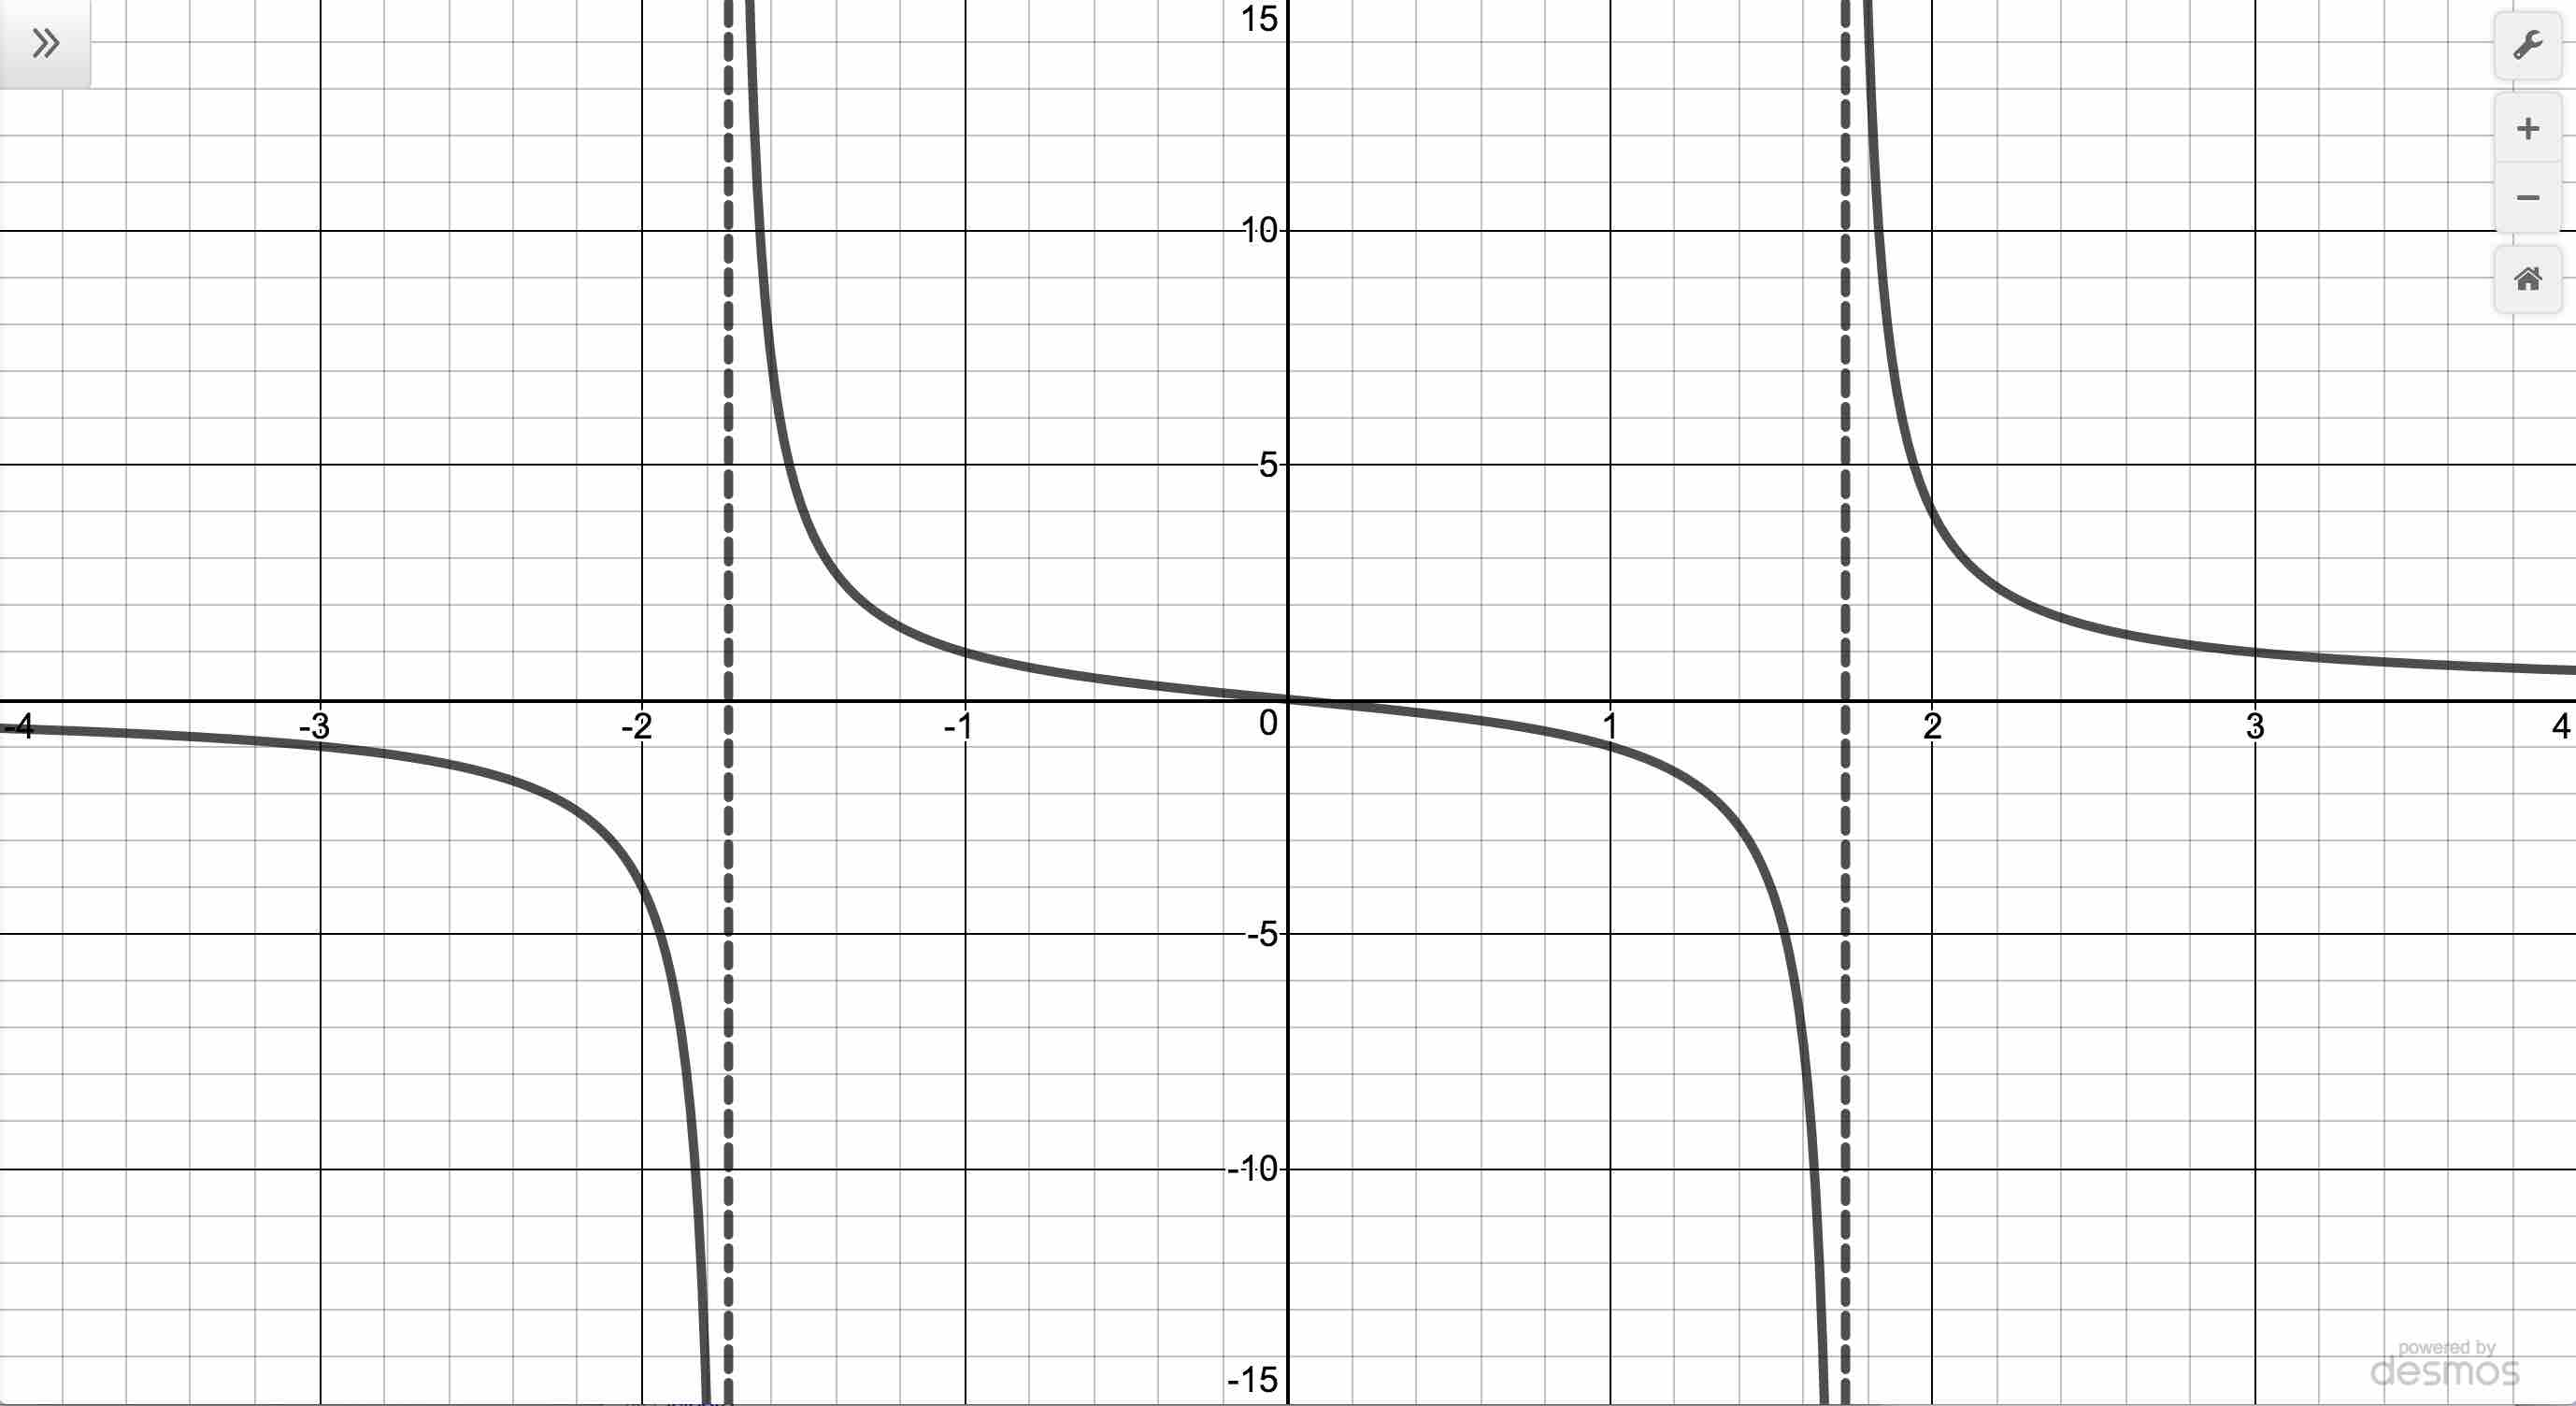
\includegraphics[width=3in]{./IntroRationalGraphics/VAorHoleEx01.jpg} & 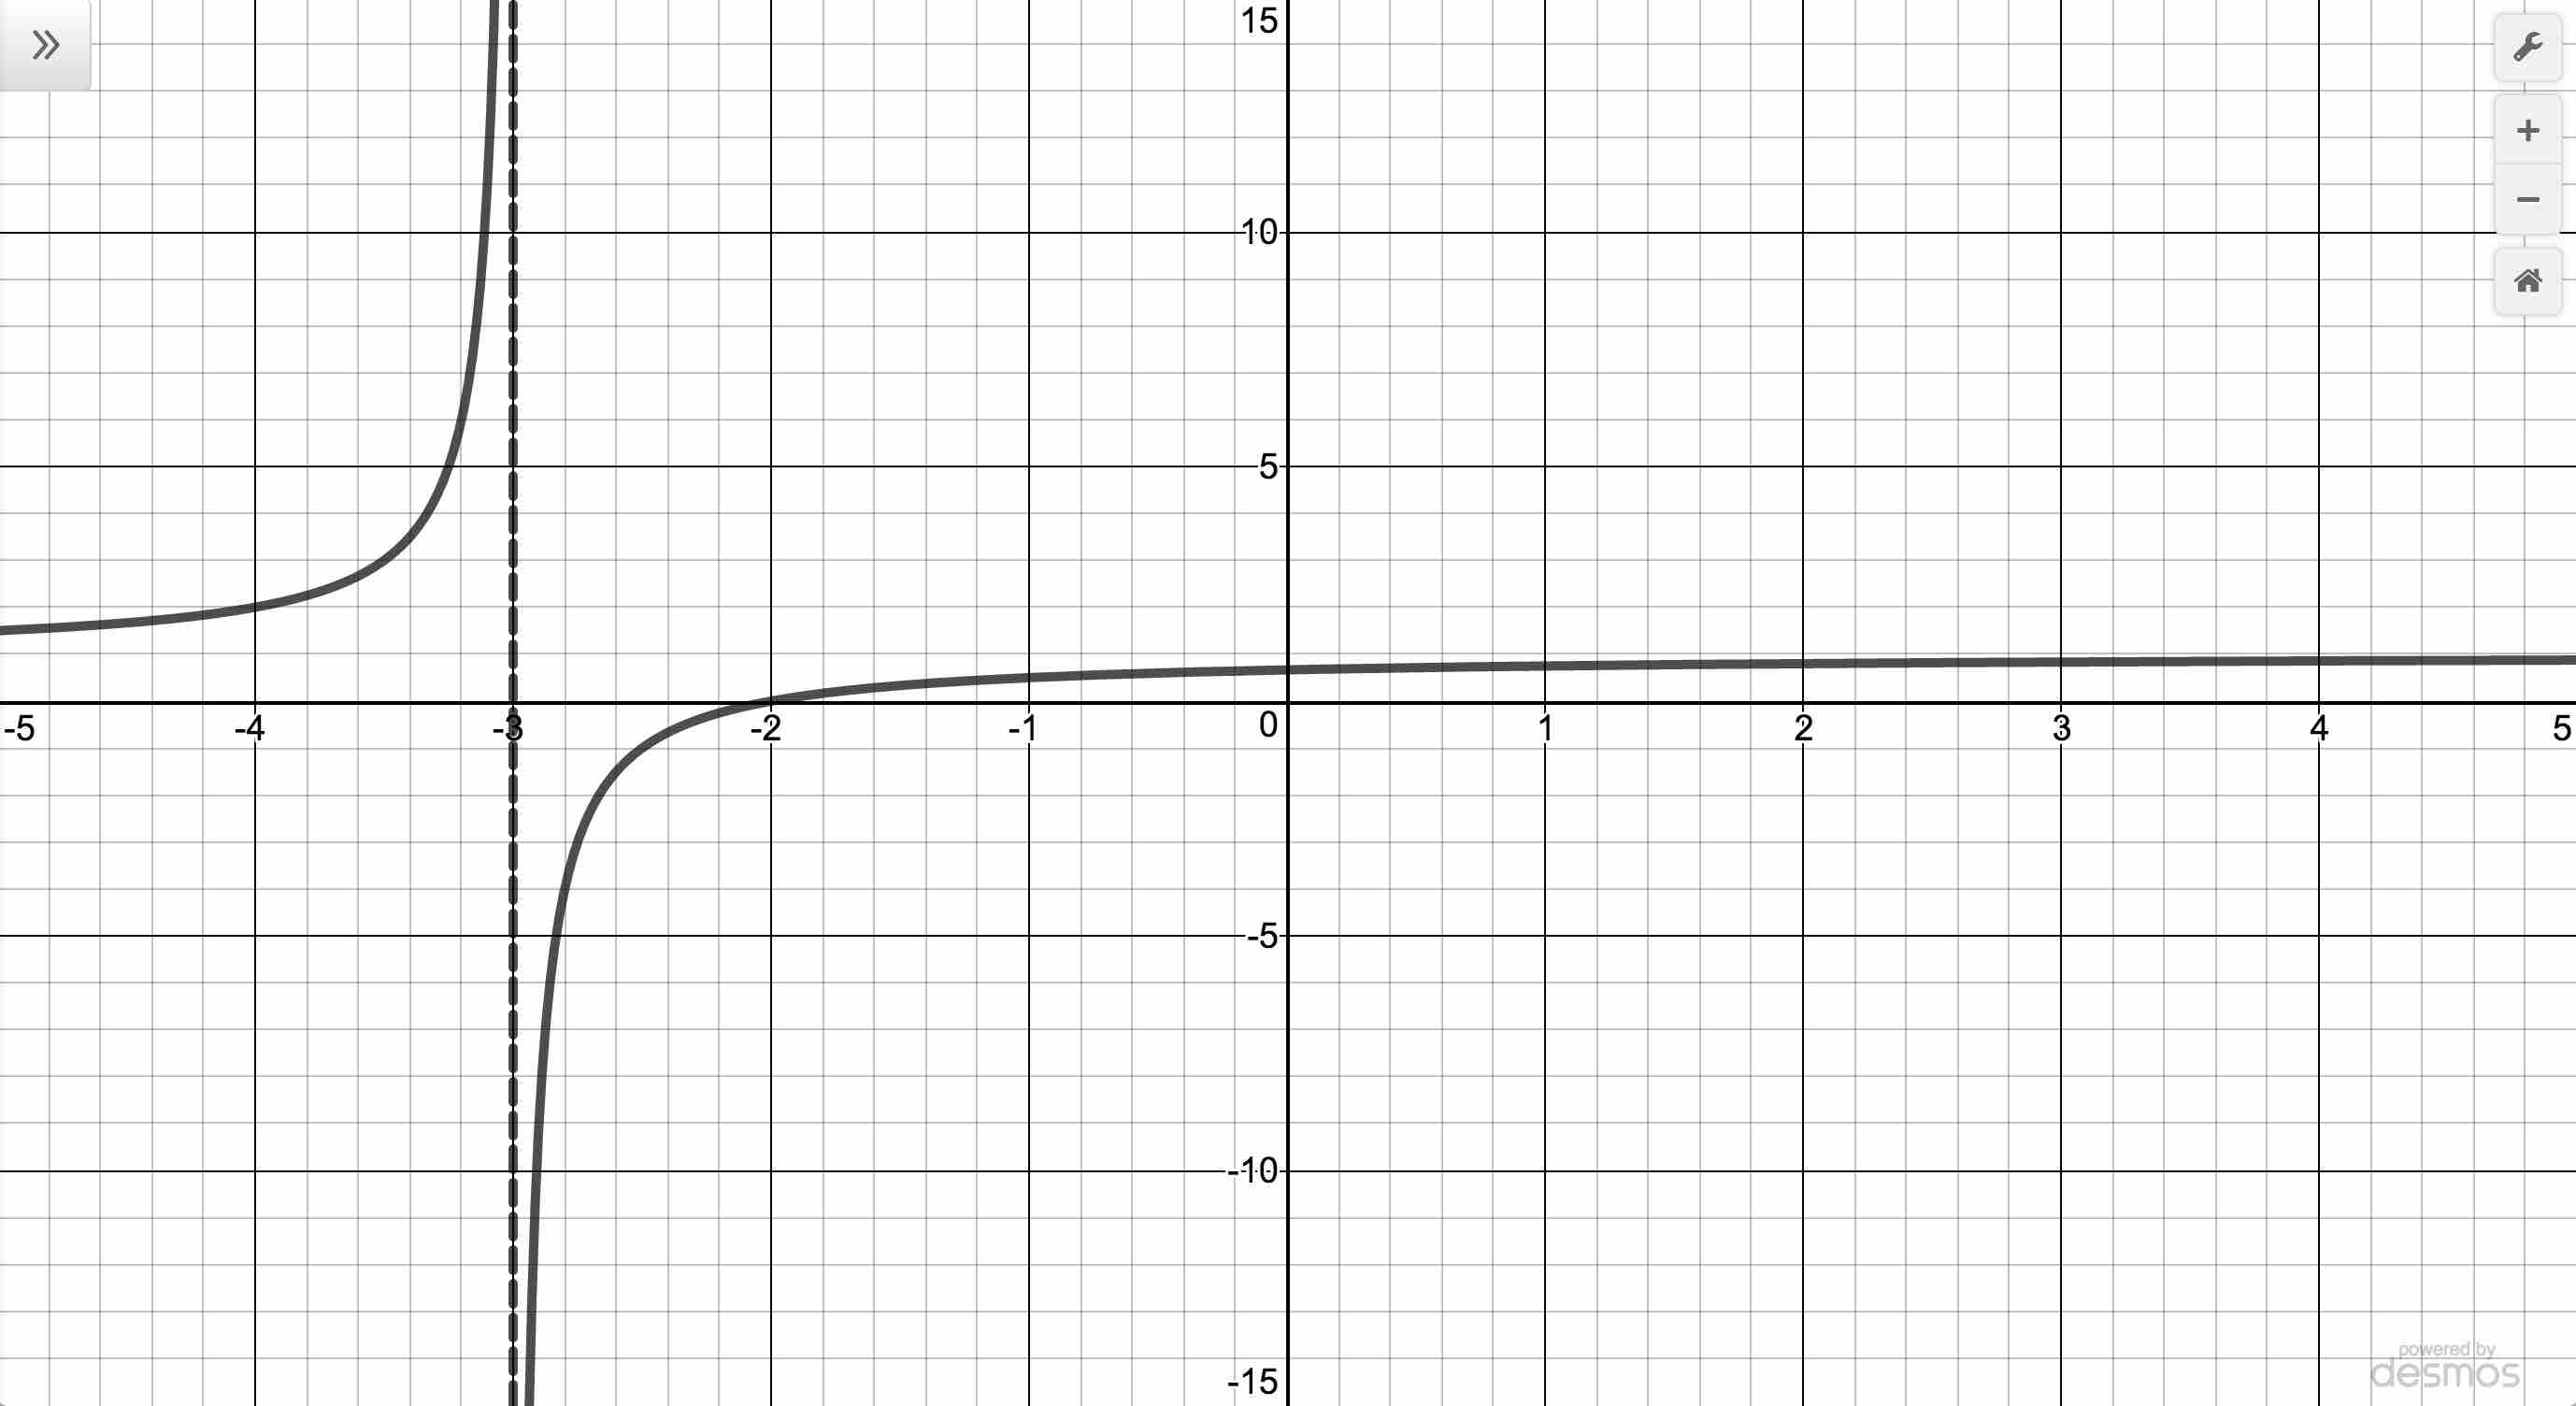
\includegraphics[width=3in]{./IntroRationalGraphics/VAorHoleEx02.jpg} \\

The graph of $y=f(x)$  \hspace{0.75in} & The graph of $y=g(t)$ \\


\end{tabular}
\end{center} 

\item  Setting the denominator of the expression for $h(t)$ to $0$ gives $t^2+9 = 0$, which has no real solutions.  Accordingly, the graph of $y=h(t)$ (at least as much as we can discern from the technology) is devoid of both vertical asymptotes and holes.  Using terms defined in Section \ref{GraphsofPolynomials},  the function $h$ is both continuous and smooth.\footnote{We'll remind you more about continuous functions in Section \ref{RationalGraphs}  \ldots}

\item  Setting the denominator of $r(t)$ to zero gives the equation $t^2+4t+4 = 0$.  We get  the (repeated!) solution $t=-2$.  Simplifying, we get  $\frac{t^2-t-6}{t^2+4t+4} = \frac{(t-3)(t+2)}{(t+2)(t+2)}  =  \frac{(t-3)\cancel{(t+2)}}{(t+2)\cancel{(t+2)}} =  \frac{t-3}{t+2}$.  Since  not all factors of $(t+2)$ cancelled from the denominator, $t=-2$ continues to produce a $0$ in the denominator.  Hence $t=-2$ is a vertical asymptote to the graph.  A graphing utility bears this out.  Specifically,     $\ds{\lim_{t \rightarrow -2^{-}} r(t) = \infty}$ and  $\ds{\lim_{t \rightarrow -2^{+}} r(t) = -\infty}$ .

\begin{center}

\begin{tabular}{cc}

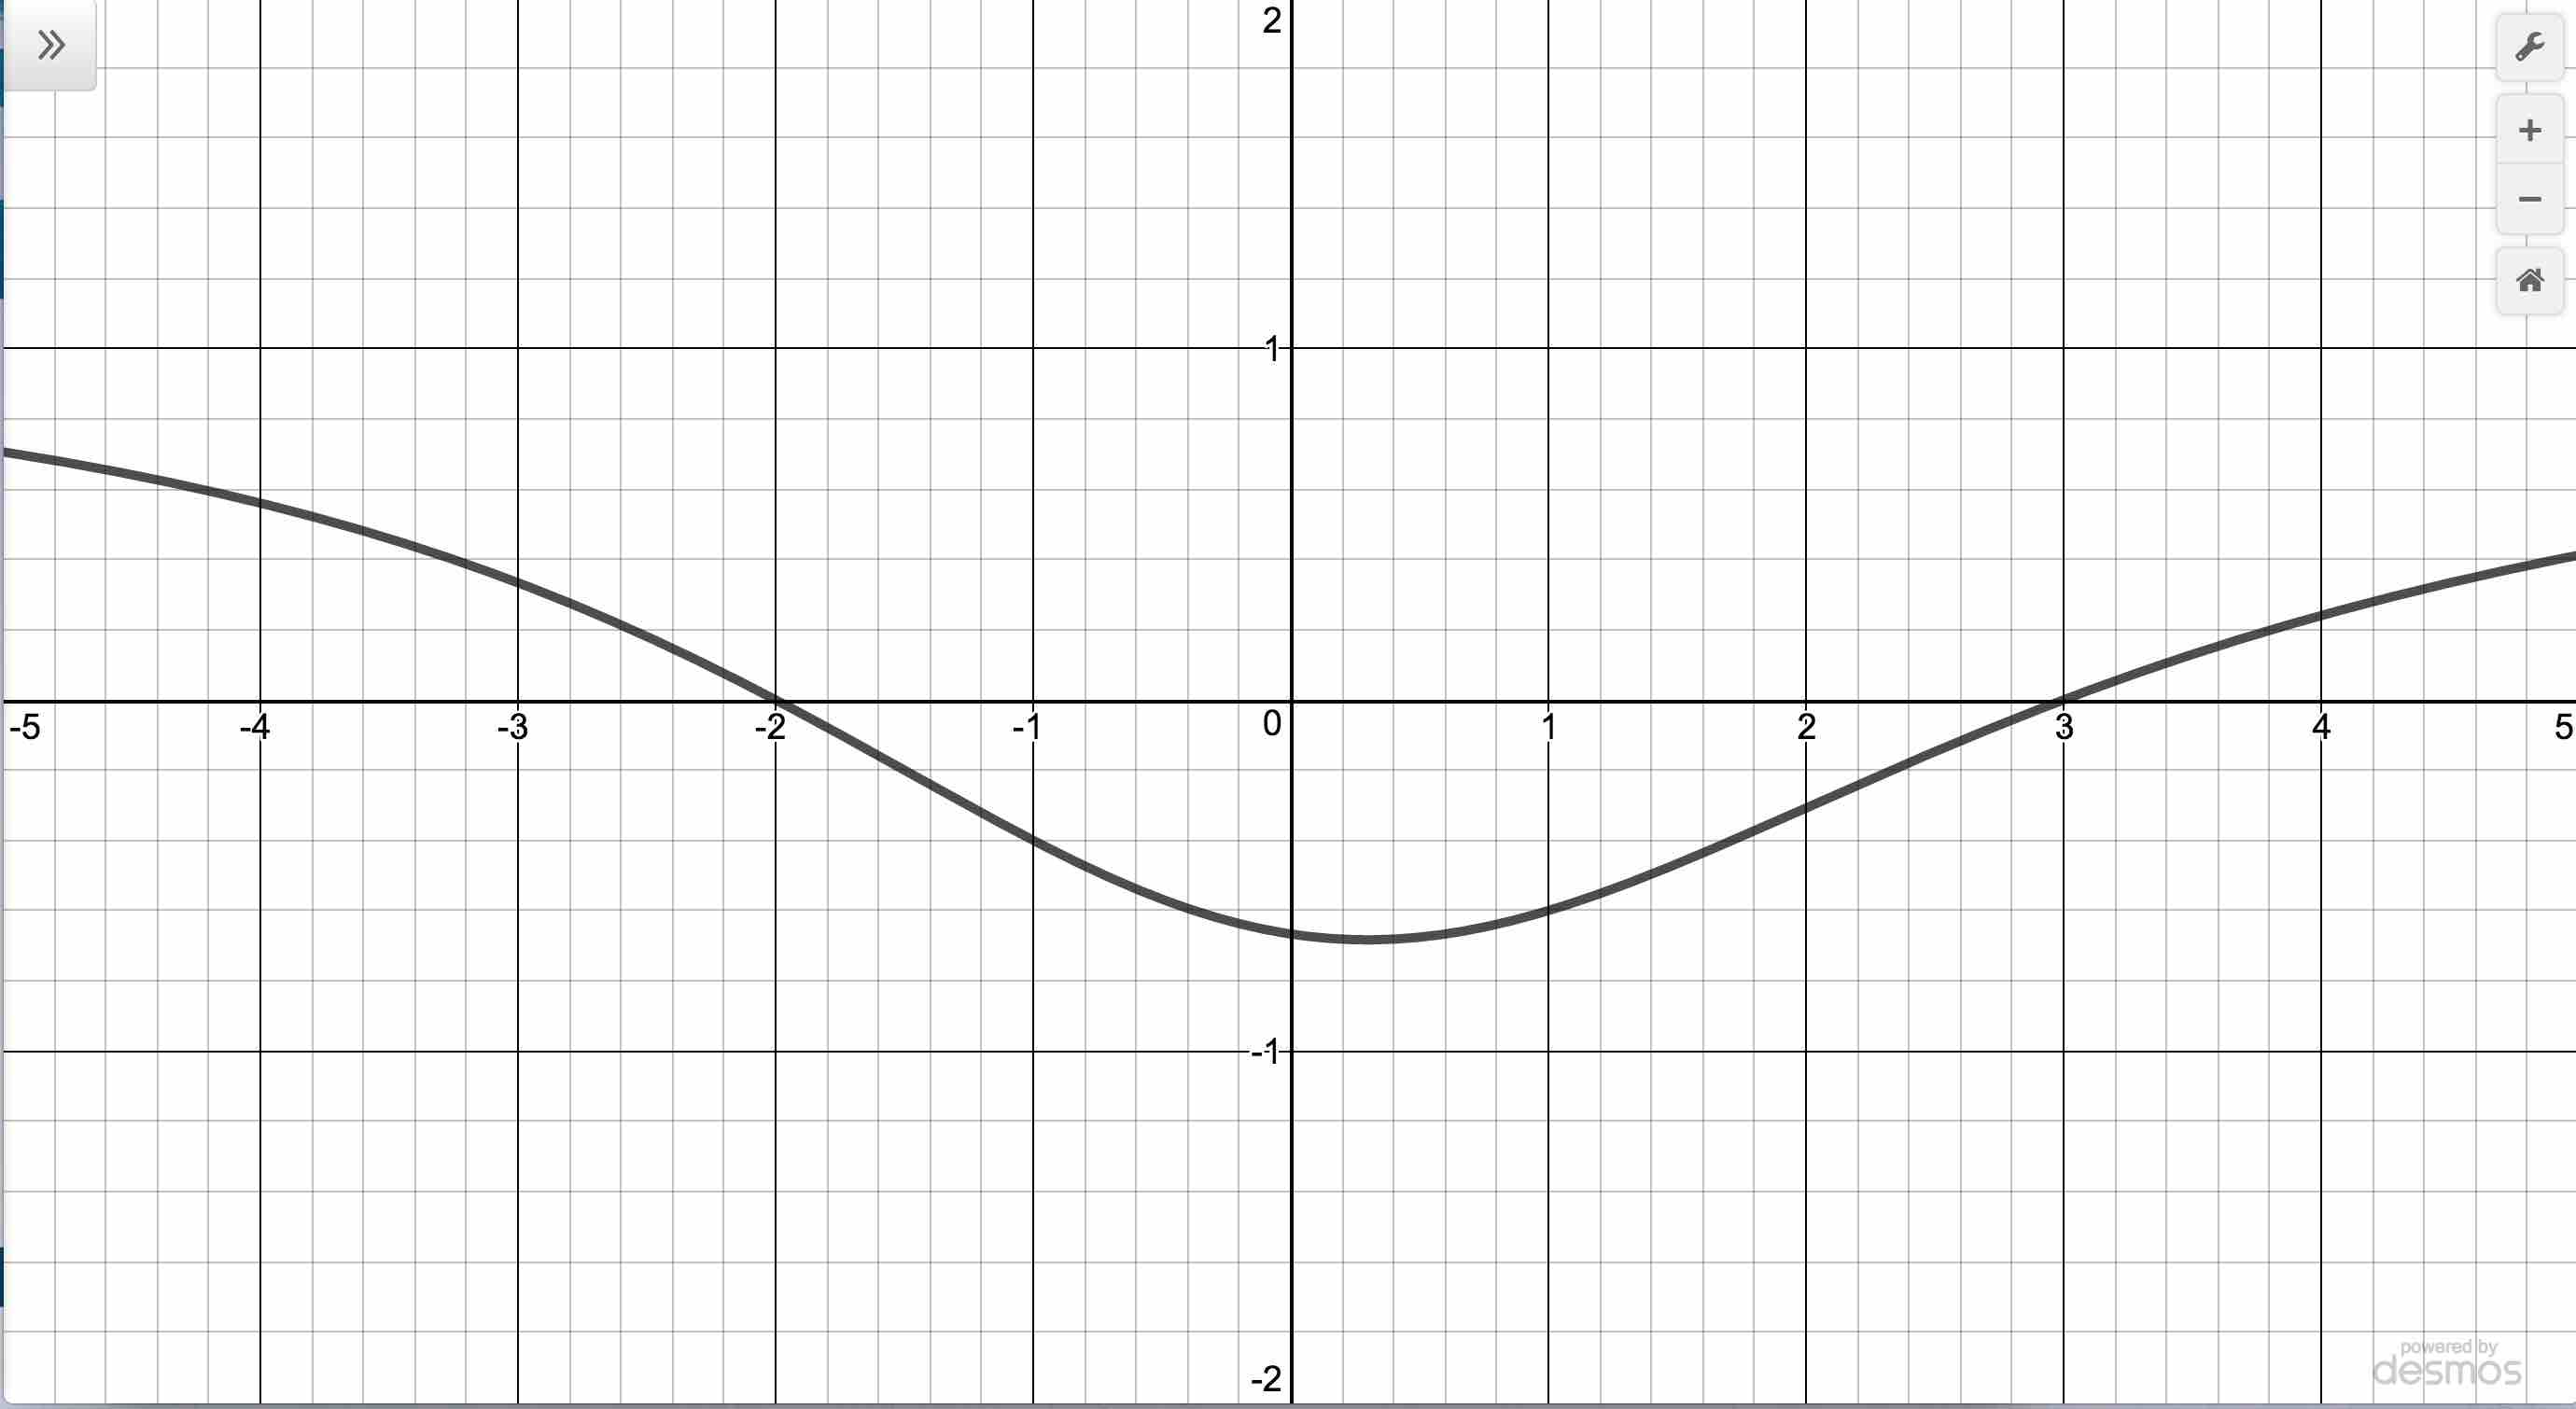
\includegraphics[width=3in]{./IntroRationalGraphics/VAorHoleEx03.jpg} & 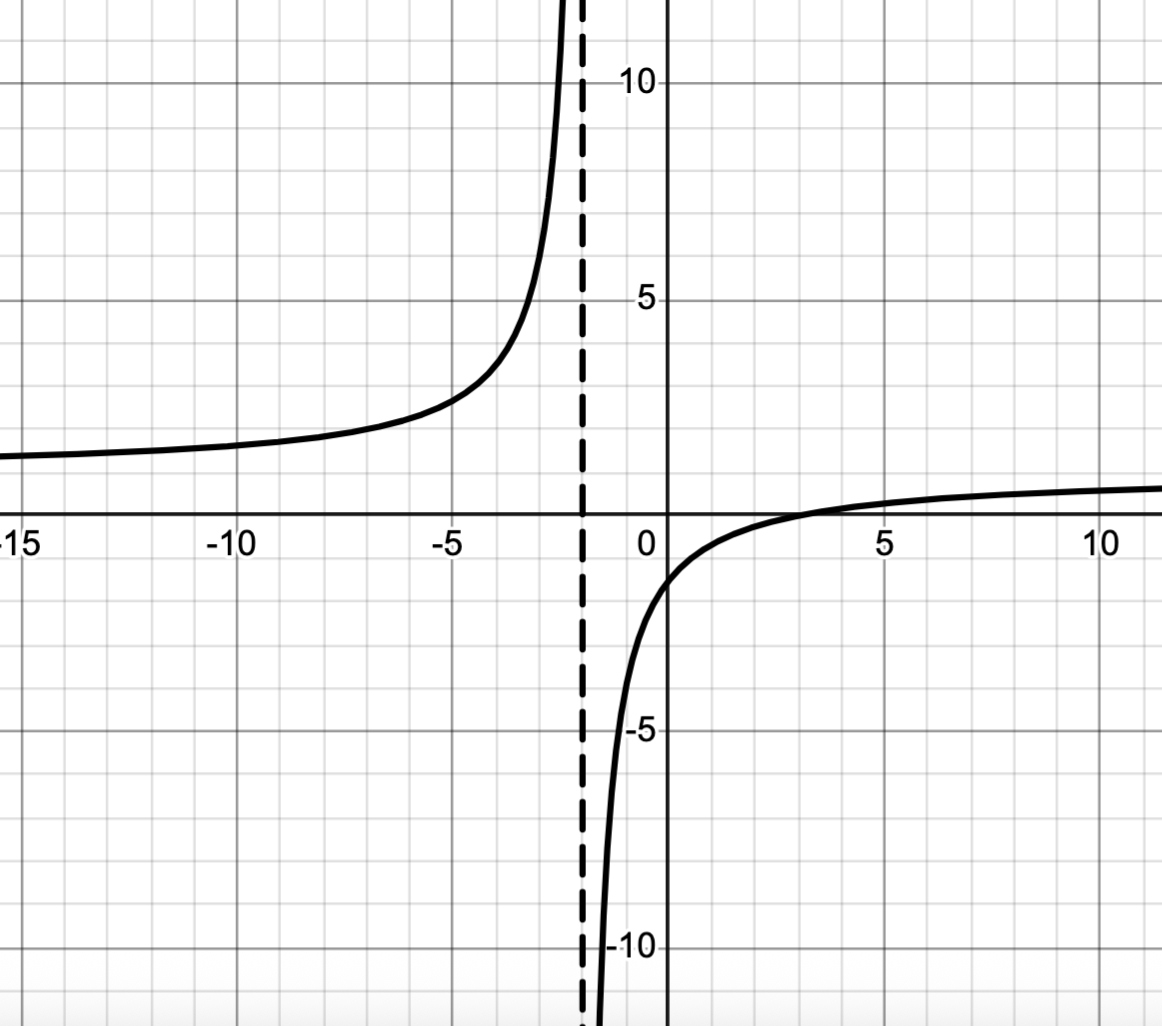
\includegraphics[width=3in]{./IntroRationalGraphics/VAorHoleEx04.png} \\

The graph of $y=h(t)$  \hspace{0.75in} & The graph of $y=r(t)$ \\


\end{tabular}
\end{center} 

\end{enumerate}
\qed
\end{ex}

\subsection{End Behavior}
\label{ebrationalsection}

Now that we've  discussed behavior near values excluded from the domains of rational functions, let's focus our attention on  end behavior.  We have already seen one example of this in the form of horizontal asymptotes.  Our next example of the section gives us a real-world application of a horizontal asymptote.\footnote{Though the population below is more accurately modeled with the functions in Chapter \ref{ExponentialandLogarithmicFunctions}, we approximate it (using Calculus, of course!) using a rational function.}

\begin{ex}  \label{fluex} The number of students $N(t)$ at local college who have had the flu $t$ months after the semester begins can be modeled by: \[ N(t) = \dfrac{1500t + 50}{3t+1},  \quad t \geq 0.\]

\begin{enumerate}

\item  Find and interpret $N(0)$.

\item  How long will it take until $300$ students will have had the flu?

\item  Use Theorem \ref{linearlaurentlgraphs} to graph $y = N(t)$.  

\item  Find and interpret $\ds{\lim_{t \rightarrow \infty} N(t)}$.

\end{enumerate}

{ \bf Solution.}

\begin{enumerate}

\item  Substituting $t=0$ gives $N(0) = \frac{1500(0) + 50}{1+3(0)} = 50$.  Since $t$ represents the number of months since the beginning of the semester, $t=0$ describes the state of the flu outbreak at the beginning of the semester. Hence,  at the beginning of the semester, $50$ students have had the flu.

\item  We set $N(t) = \frac{1500t + 50}{3t+1}  = 300$ and solve.  Clearing denominators gives $1500t + 50 = 300(3t+1)$ from which we get $t = \frac{5}{12}$.  This means it will take $\frac{5}{12}$ months, or about 13 days, for $300$ students to have had the flu.

\item To graph $y = N(t)$, we first use long division to rewrite $N(t) = \frac{-450}{3t+1} + 500$.  From there, we get  \[N(t) =  -\frac{450}{3t+1} + 500  = \frac{-450}{3\left(t + \frac{1}{3}\right)} + 500 = \frac{-150}{t+\frac{1}{3}} + 500\]

Using Theorem \ref{linearlaurentlgraphs}, we start with the graph of $y = \frac{1}{t}$ below on the left and perform the following steps: shift the graph to the left by $\frac{1}{3}$ units, stretch the graph vertically by a factor of $150$, reflect the graph across the $t$-axis, and finally, shift the graph up $500$ units.   As the domain of $N$ is $t \geq 0$, we obtain the graph below on the right.

\[ \begin{array}{ccc}


\begin{mfpic}[15]{-5}{5}{-5}{5}
\axes
\scriptsize
\tlabel[cc](5, -0.5){$t$}
\tlabel[cc](0.5, 5){$y$}
\tlabel[cc](-2, -1.5){$(-1,-1)$}
\tlabel[cc](2, 1.5){$(1,1)$}
\normalsize
\penwd{1.25pt}
\arrow \reverse \arrow \function{-5,-0.2,0.1}{1/x}
\arrow \reverse \arrow \function{0.2,5,0.1}{1/x}
\point[4pt]{(-1,-1), (1,1)}
\tcaption{\scriptsize $y =  \frac{1}{t}$}
\end{mfpic}


&
\stackrel{\text{Theorem \ref{linearlaurentlgraphs}}}{\xrightarrow{\hspace{1.5in}}}

&

\begin{mfpic}[15]{-1}{9}{-1}{9}
\axes
\dashed \polyline{(-1,5), (9,5)}
\scriptsize
\tlabel[cc](9, -0.5){$t$}
\tlabel[cc](0.5, 9){$y$}
\tlabel[cc](7, 5.5){$y = 500$}
\tlabel[cc](-1, 0.5){$(0,50)$}
\tlabel[cc](1.75, 3.25){$\left(\frac{2}{3},350 \right)$}
\normalsize
\penwd{1.25pt}
\arrow \function{0,9,0.1}{5 - (1.5/(x+1/3))}
\point[4pt]{(0,0.5), (0.6666,3.5)}
\tcaption{\scriptsize $y=N(t)$}
\end{mfpic}
 \\

 \text{\scriptsize  $(-1,1)$ , $(1,1)$,  HA: $y=0$} & & \text{\scriptsize $\left(\frac{2}{3},350 \right)$, HA: $y = 500$  } \\
 
 \end{array} \]


  
\item  Owing to the horizontal asymptote, $y =500$, we have $\ds{\lim_{t \rightarrow \infty} N(t) = 500}$. (More specifically, as $t \rightarrow \infty$,  $N(t) \rightarrow 500^{-}$.)  This means as time goes by, only a total of 500 students will have ever had the flu. \qed

\end{enumerate}

\end{ex}
 
 We determined the horizontal asymptote to the graph of $y = N(t)$ in Example \ref{fluex} by rewriting $N(t)$ into a form compatible with Theorem  \ref{linearlaurentlgraphs}, and while there is nothing wrong with this approach, it will simply not work for general rational functions which cannot be rewritten this way.  To that end, we revisit this problem using Theorem \ref{EBPolynomials} from Section \ref{GraphsofPolynomials}.  The end behavior of the numerator of $N(t) = \frac{1500t + 50}{3t+1}$ is determined by its leading term,  $1500t$,  and the end behavior of the denominator is likewise determined  by its leading term, $3t$.  Hence, as $t \rightarrow  \infty$:
 
 \[ N(t) = \dfrac{1500t + 50}{3t+1} \approx \dfrac{1500t}{3t} = 500.\]
 
Hence $\ds{\lim_{t \rightarrow  \infty} N(t) = 500}$ so  $y = 500$ is the horizontal asymptote.  This same reasoning can be used in general to argue the following theorem.

\smallskip
\colorbox{ResultColor}{\bbm

\begin{thm} \index{asymptote ! horizontal ! location of}\index{horizontal asymptote ! location of}\textbf{Location of Horizontal Asymptotes:}\label{hathm} Suppose $r$ is a rational function and $r(x) = \frac{p(x)}{q(x)}$, where $p$ and $q$ are polynomial functions with leading coefficients $a$ and $b$, respectively. 

\begin{itemize}

\item  If the degree of $p(x)$ is the same as the degree of $q(x)$, then $\ds{\lim_{x \rightarrow \infty} r(x) =}$ $\frac{a}{b}$ so $y=\frac{a}{b}$ is the\footnote{The use of the definite article will be justified momentarily.} horizontal asymptote of the graph of $y=r(x)$.

\item  If the degree of $p(x)$ is less than the degree of $q(x)$, then $\ds{\lim_{x \rightarrow \infty} r(x) =0}$  so $y=0$ (the $x$-axis) is the horizontal asymptote of the graph of $y=r(x)$.

\item  If the degree of $p(x)$ is greater than the degree of $q(x)$, then the graph of $y=r(x)$ has no horizontal asymptotes.


\end{itemize}
\end{thm}
\ebm}
\smallskip



So see why Theorem \ref{hathm} works, suppose $r(x) = \frac{p(x)}{q(x)}$ where $a$ is the leading coefficient of $p(x)$ and $b$ is the leading coefficient of $q(x)$. As $x \rightarrow  -\infty$ or $x \rightarrow \infty$,  Theorem \ref{EBPolynomials} gives $r(x) \approx \frac{ax^n}{bx^m}$, where $n$ and $m$ are the degrees of $p(x)$ and $q(x)$, respectively. 

If the degree of $p(x)$ and the degree of $q(x)$ are the same, then $n=m$ so that $r(x) \approx \frac{ax^n}{bx^n} = \frac{a}{b}$.  Hence $\ds{\lim_{x \rightarrow  -\infty} r(x)}$ $=\frac{a}{b}$  and $\ds{\lim_{x \rightarrow  \infty} r(x)}$ $=\frac{a}{b}$ which means $y=\frac{a}{b}$ is the horizontal asymptote in this case.  

If the degree of $p(x)$ is less than the degree of $q(x)$, then $n < m$, so $m-n$ is a positive number, and hence, $r(x) \approx  \frac{ax^n}{bx^m}  = \frac{a}{bx^{m-n}} \rightarrow 0$.   As $x \rightarrow  -\infty$ or $x \rightarrow \infty$, $r(x)$ is more or less a fraction with a constant numerator, $a$, but a denominator which is unbounded. Hence, $\ds{\lim_{x \rightarrow  -\infty} r(x) = 0}$ and $\ds{\lim_{x \rightarrow  \infty} r(x) = 0}$  producing the horizontal asymptote $y = 0$.   

If the degree of $p(x)$ is greater than the degree of $q(x)$, then $n > m$, and hence $n-m$ is a positive number and $r(x) \approx  \frac{ax^n}{bx^m}  = \frac{ax^{n-m}}{ b}$, which is a monomial function from Section \ref{GraphsofPolynomials}.  As such, $r$ becomes unbounded as $x \rightarrow -\infty$ or $x \rightarrow \infty$.

Note that in the two cases which produce horizontal asymptotes, the behavior of $r$ is identical as $x \rightarrow -\infty$ and $x \rightarrow \infty$.  Hence, if the graph of a rational function has a horizontal asymptote, there is only one.\footnote{We will (first) encounter functions with more than one horizontal asymptote in Chapter \ref{RootRadicalFunctions}.} 

We put Theorem \ref{hathm}  to good use in the following example.
 
\begin{ex} \label{haexample} For each function below:

\begin{itemize}

\item use Theorem \ref{EBPolynomials} to  analytically determine the horizontal asymptotes to the graph, if any.

\item check your answers Theorem \ref{hathm} and a graphing utility.   

\item describe the end behavior of the graph using proper notation.

\item  investigate any apparent symmetry of the graph about the $y$-axis or origin.

\end{itemize}

\begin{multicols}{2}
\begin{enumerate}

\item $F(s) = \dfrac{5s}{s^2+1}$  \vphantom{ $g(x) = \dfrac{x^2-4}{x+1}$}

\item  $g(x) = \dfrac{x^2-4}{x+1}$ 

\setcounter{HW}{\value{enumi}}
\end{enumerate}
\end{multicols}

\begin{multicols}{2}
\begin{enumerate}
\setcounter{enumi}{\value{HW}}


\item  $h(t) = \dfrac{6t^3-3t+1}{5-2t^3}$

\item  $r(x) = 2 - \dfrac{3x^2}{1-x^2}$ \vphantom{ $h(t) = \dfrac{6t^3-3t+1}{5-2t^3}$}

\setcounter{HW}{\value{enumi}}
\end{enumerate}
\end{multicols}


{ \bf Solution.}

\begin{enumerate}

\item  Using  Theorem \ref{EBPolynomials}, we get as $s \rightarrow  -\infty$ or $s \rightarrow \infty$, $F(s) = \frac{5s}{s^2+1}  \approx \frac{5s}{s^2} = \frac{5}{s}$.  Hence, $\ds{\lim_{s \rightarrow  -\infty} F(s) = 0}$ and $\ds{\lim_{s \rightarrow  \infty} F(s) = 0}$   so $y = 0$ is a horizontal asymptote to the graph.  

Alternatively, to use Theorem \ref{hathm} note the degree of the numerator of  $F(s)$,  $1$, is less than the degree of the denominator, $2$,  so  $y=0$ as the horizontal asymptote using this approach as well.

Graphically, as $s \rightarrow  -\infty$ or $s \rightarrow  \infty$ , the graph $y = F(s)$ approaches the $s$-axis ($y = 0$).  More specifically, as $s \rightarrow -\infty$, $F(s)  \rightarrow 0^{-}$ and as $s \rightarrow \infty$, $F(s)  \rightarrow 0^{+}$.  

As a side note, the graph of $F$ appears to be symmetric about the origin.  Indeed, $F(-s) = \frac{5(-s)}{(-s)^2+1} = -\frac{5s}{s^2+1}$ proving $F$ is odd.

\item  As $x \rightarrow  -\infty$ or $x \rightarrow \infty$, $g(x) = \frac{x^2-4}{x+1} \approx \frac{x^2}{x} = x$, and while $y = x$ is a line, it is not a horizontal line.  Hence, we conclude the graph of $y = g(x)$ has no horizontal asymptotes.  Sure enough,  Theorem \ref{hathm} supports this since the degree of the numerator of $g(x)$ is $2$ which is greater than the degree of the denominator, $1$.   From the graph, we see that the graph of $y=g(x)$ doesn't appear to level off to a constant value, confirming there is no horizontal asymptote.\footnote{Sit tight!  We'll revisit this function and its end behavior shortly.}

\begin{center}
\begin{tabular}{cc}

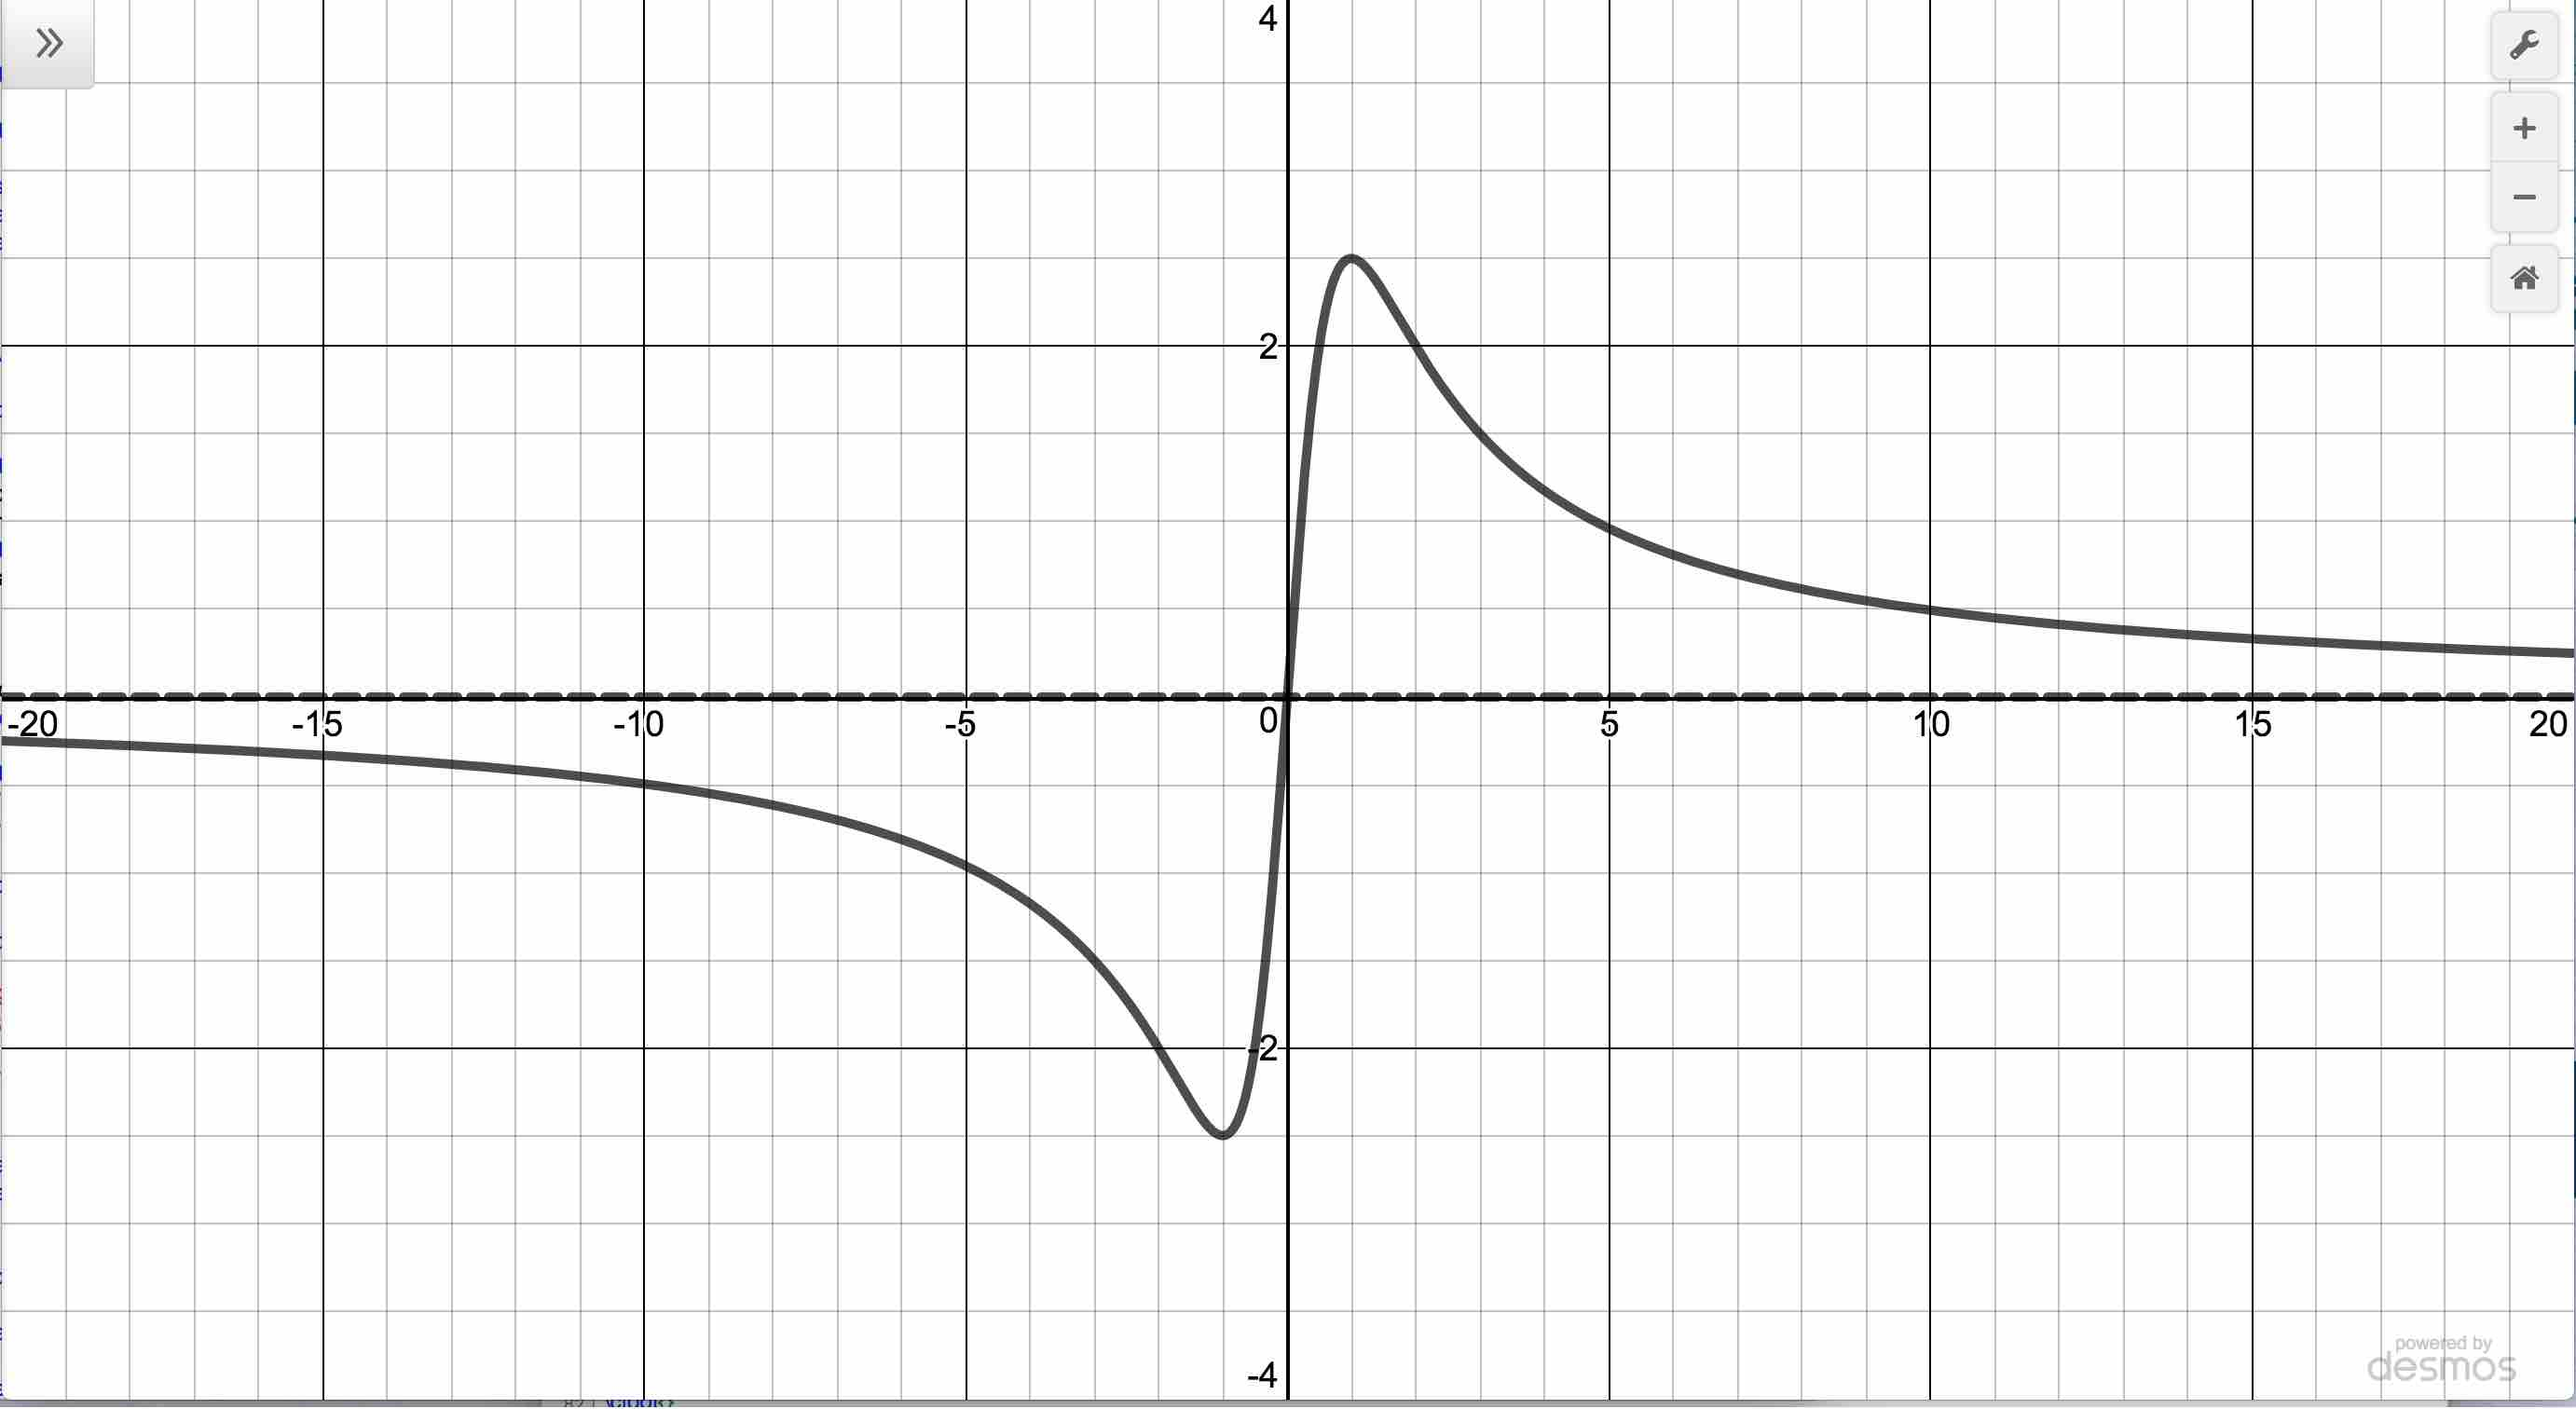
\includegraphics[width=3in]{./IntroRationalGraphics/HAEx01.jpg}  & 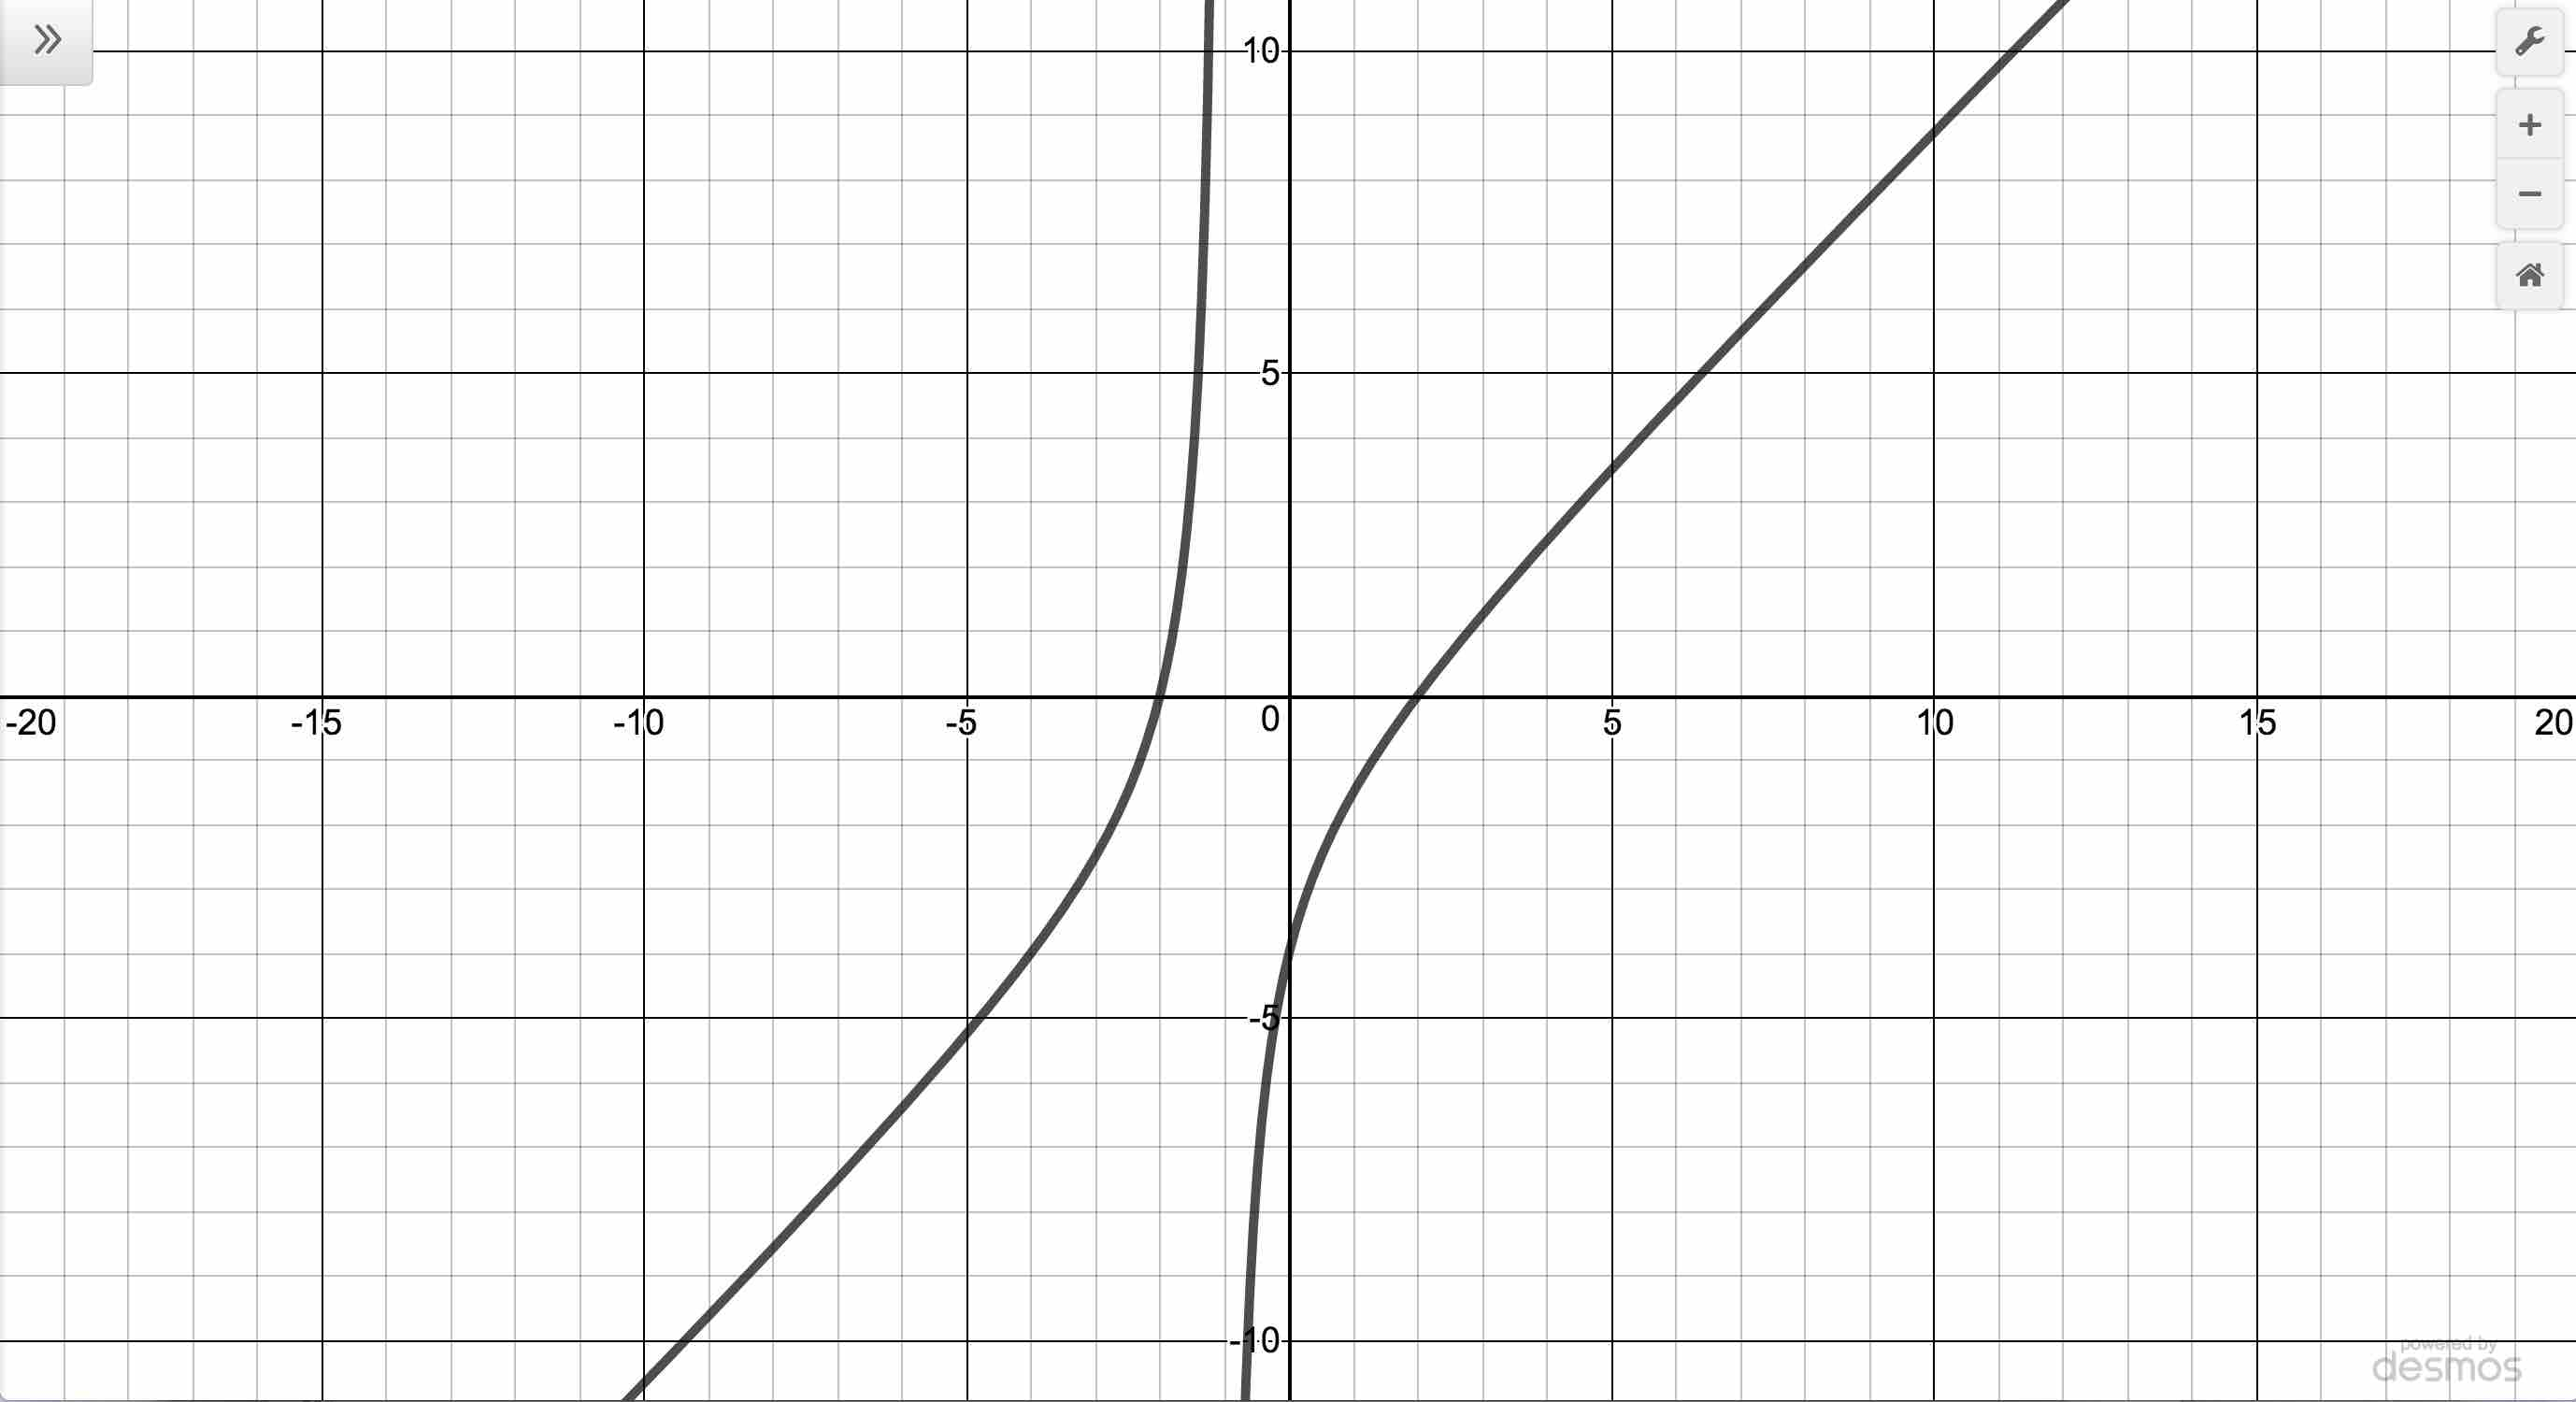
\includegraphics[width=3in]{./IntroRationalGraphics/HAEx02.jpg} \\
The graph of $y=F(s)$  & The graph of $y=g(x)$ \\


\end{tabular}
\end{center} 

\item   As $t \rightarrow -\infty$ or $t \rightarrow \infty$,  $h(t) = \frac{6t^3-3t+1}{5-2t^3} \approx  \frac{6t^3}{-2t^3} = -3$.  Hence, $\ds{\lim_{t \rightarrow  -\infty} h(t) = -3}$ and $\ds{\lim_{t \rightarrow  \infty} h(t) = -3}$, indicating a horizontal asymptote $y = -3$.  Sure enough, since the degrees of the numerator and denominator of $h(t)$ are both three,  Theorem \ref{hathm} tells us $y = \frac{6}{-2} = -3$ is the horizontal asymptote.  We see from the graph of $y = h(t)$ that as $t \rightarrow -\infty$, $h(t) \rightarrow -3^{+}$, and as $t \rightarrow \infty$, $h(t) \rightarrow -3^{-}$.

\item  If we apply Theorem \ref{EBPolynomials} to the term  $\frac{3x^2}{1-x^2}$ in the expression for $r(x)$, we find   $\frac{3x^2}{1-x^2} \approx \frac{3x^2}{-x^2} = -3$ as $x \rightarrow -\infty$ or $x \rightarrow \infty$.  It  seems reasonable to conclude, then, that  $\ds{\lim_{x \rightarrow  -\infty} r(x) = 2 - (-3) = 5}$ and likewise $\ds{\lim_{x \rightarrow  \infty} r(x) = 2 - (-3) = 5}$ so $y = 5$ is our horizontal asymptote. 

 In order to double check this calculation using  Theorem \ref{hathm}, however, we need to rewrite the expression $r(x)$ with a single denominator:  $r(x) = 2 - \frac{3x^2}{1-x^2} = \frac{2(1-x^2) - 3x^2}{1-x^2} = \frac{2-5x^2}{1-x^2}$.  Now we apply Theorem \ref{hathm}  and note since the numerator and denominator have the same degree, we are guaranteed the horizontal asymptote is $y = \frac{-5}{-1} = 5$.  
 
Both  calculations are borne out graphically below where it appears as if as $x \rightarrow  -\infty$ or $x \rightarrow \infty$, $r(x) \rightarrow 5^{+}$. 

 As a final note, the graph of $r$ appears to be symmetric about the $y$ axis.  We find $r(-x) = 2 - \frac{3(-x)^2}{1-(-x)^2} = 2 - \frac{3x^2}{1-x^2} = r(x)$, proving $r$ is even.

\begin{center}
\begin{tabular}{cc}

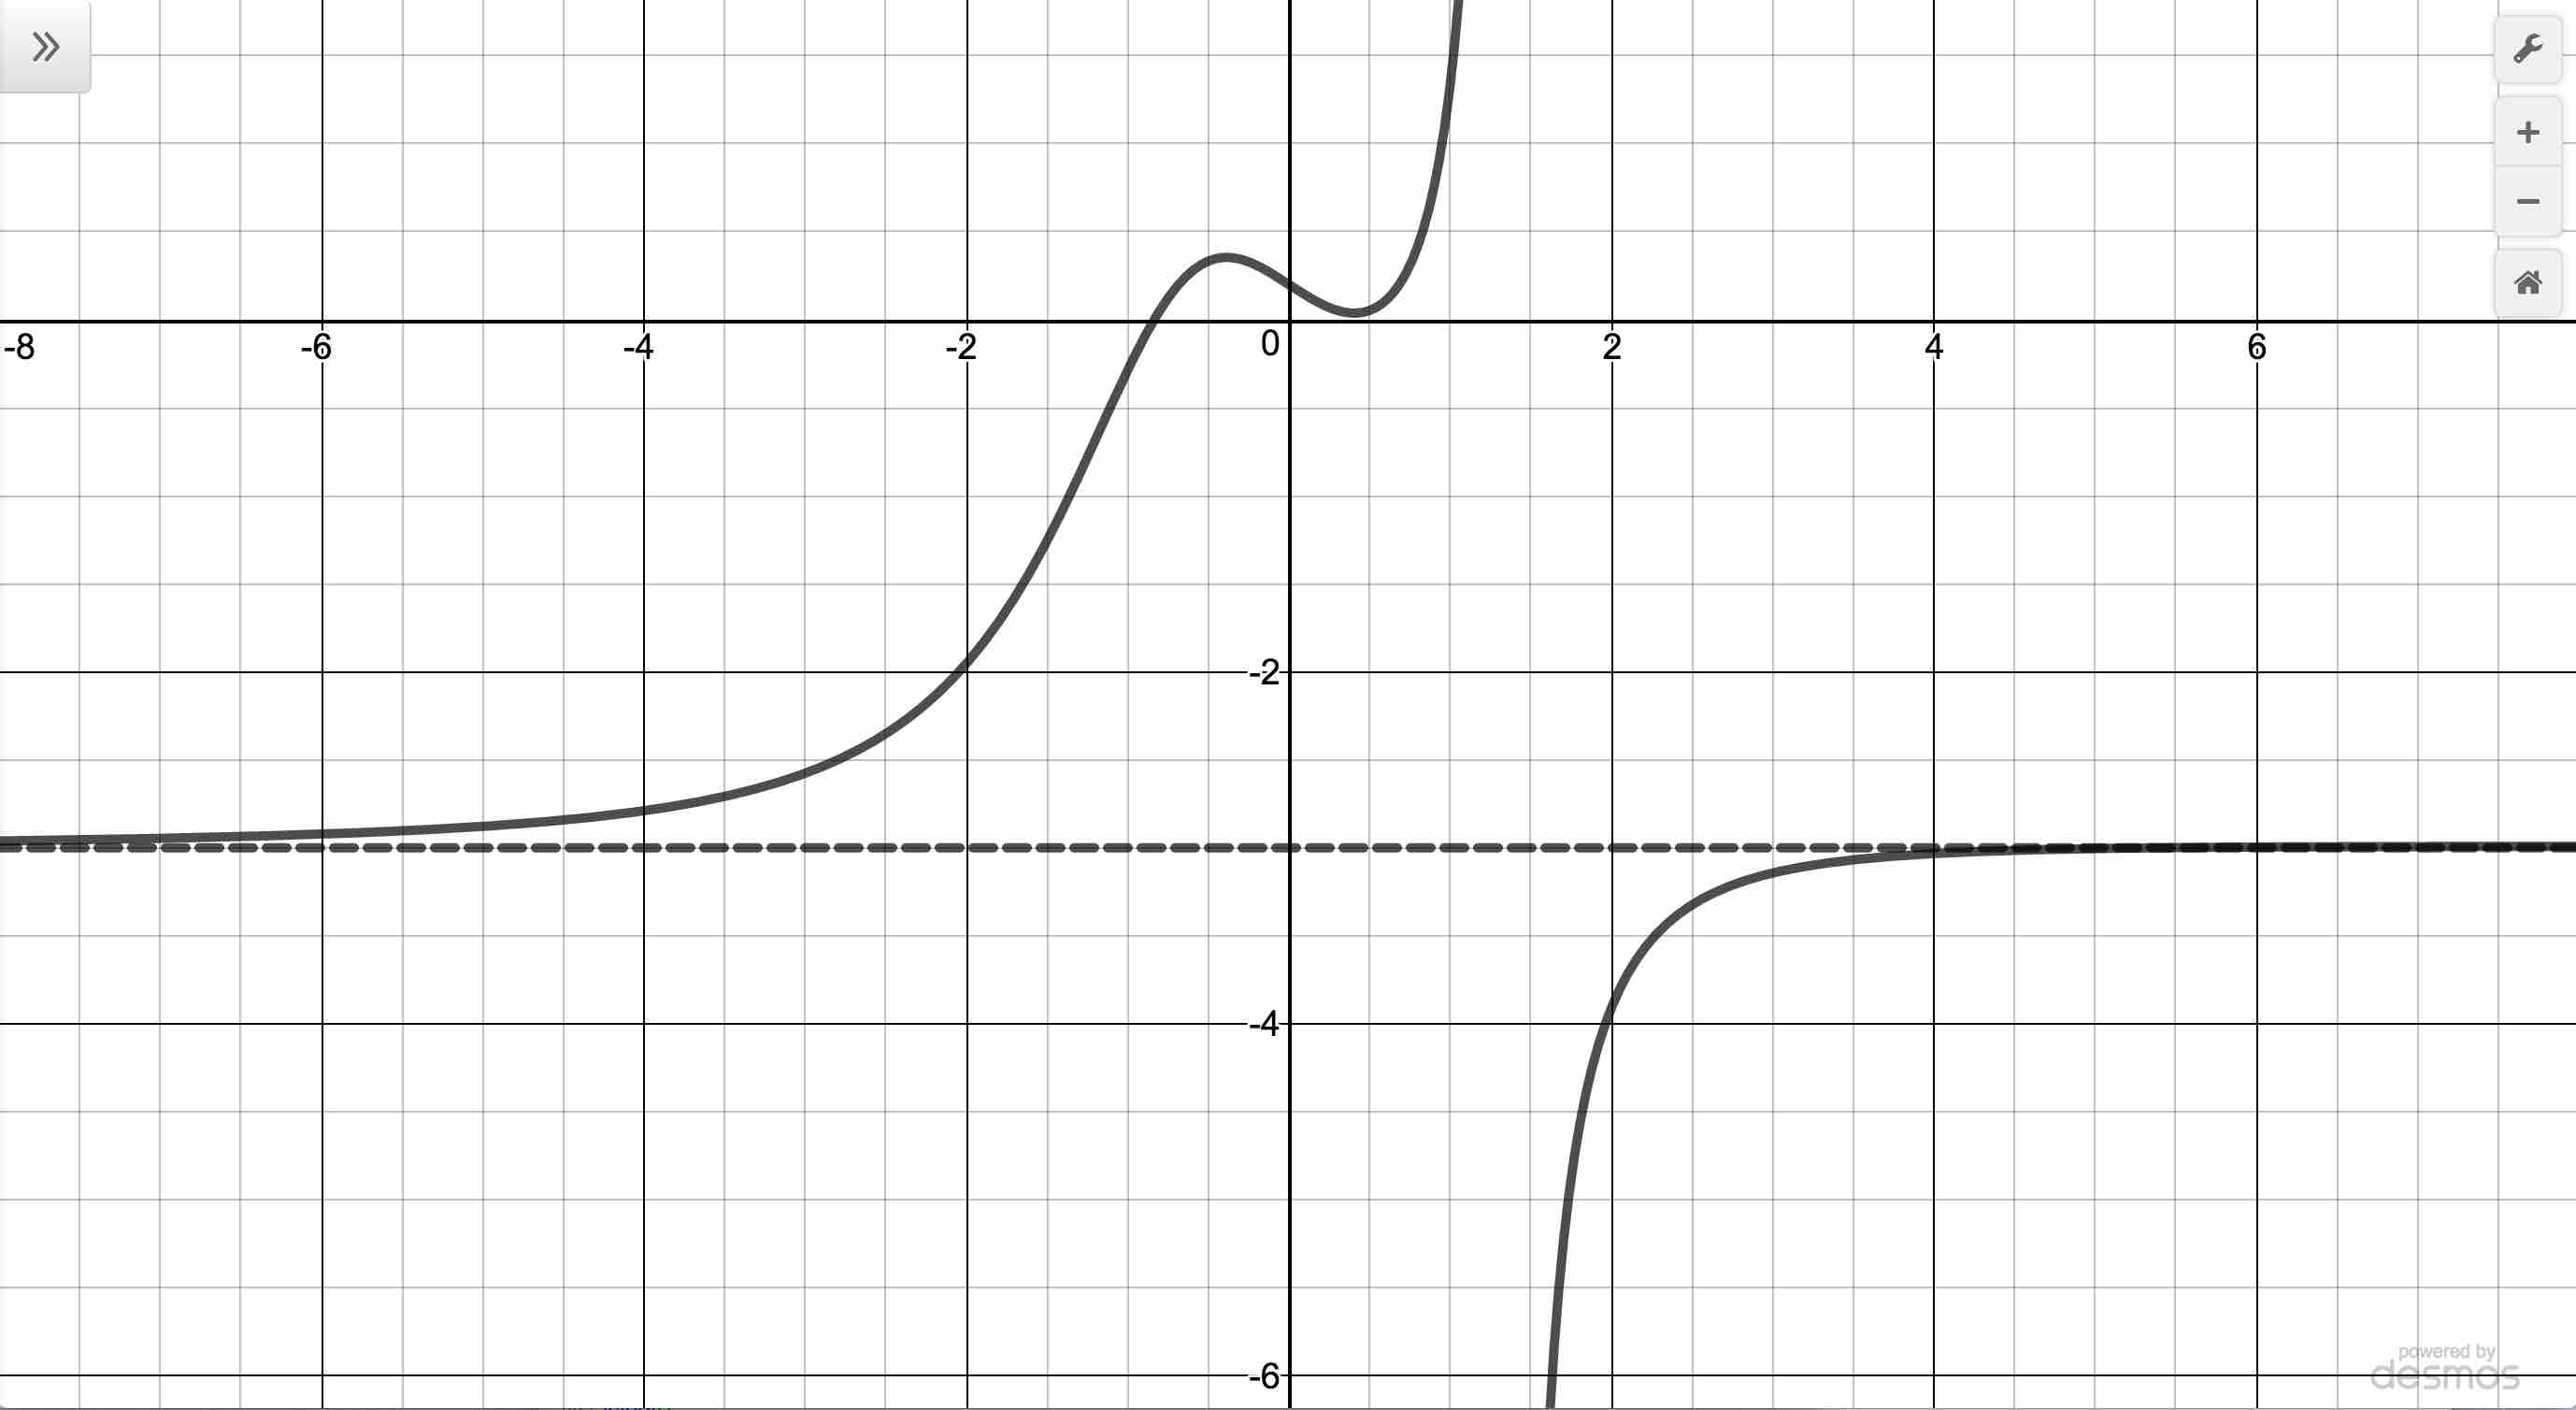
\includegraphics[width=3in]{./IntroRationalGraphics/HAEx03.jpg}  & 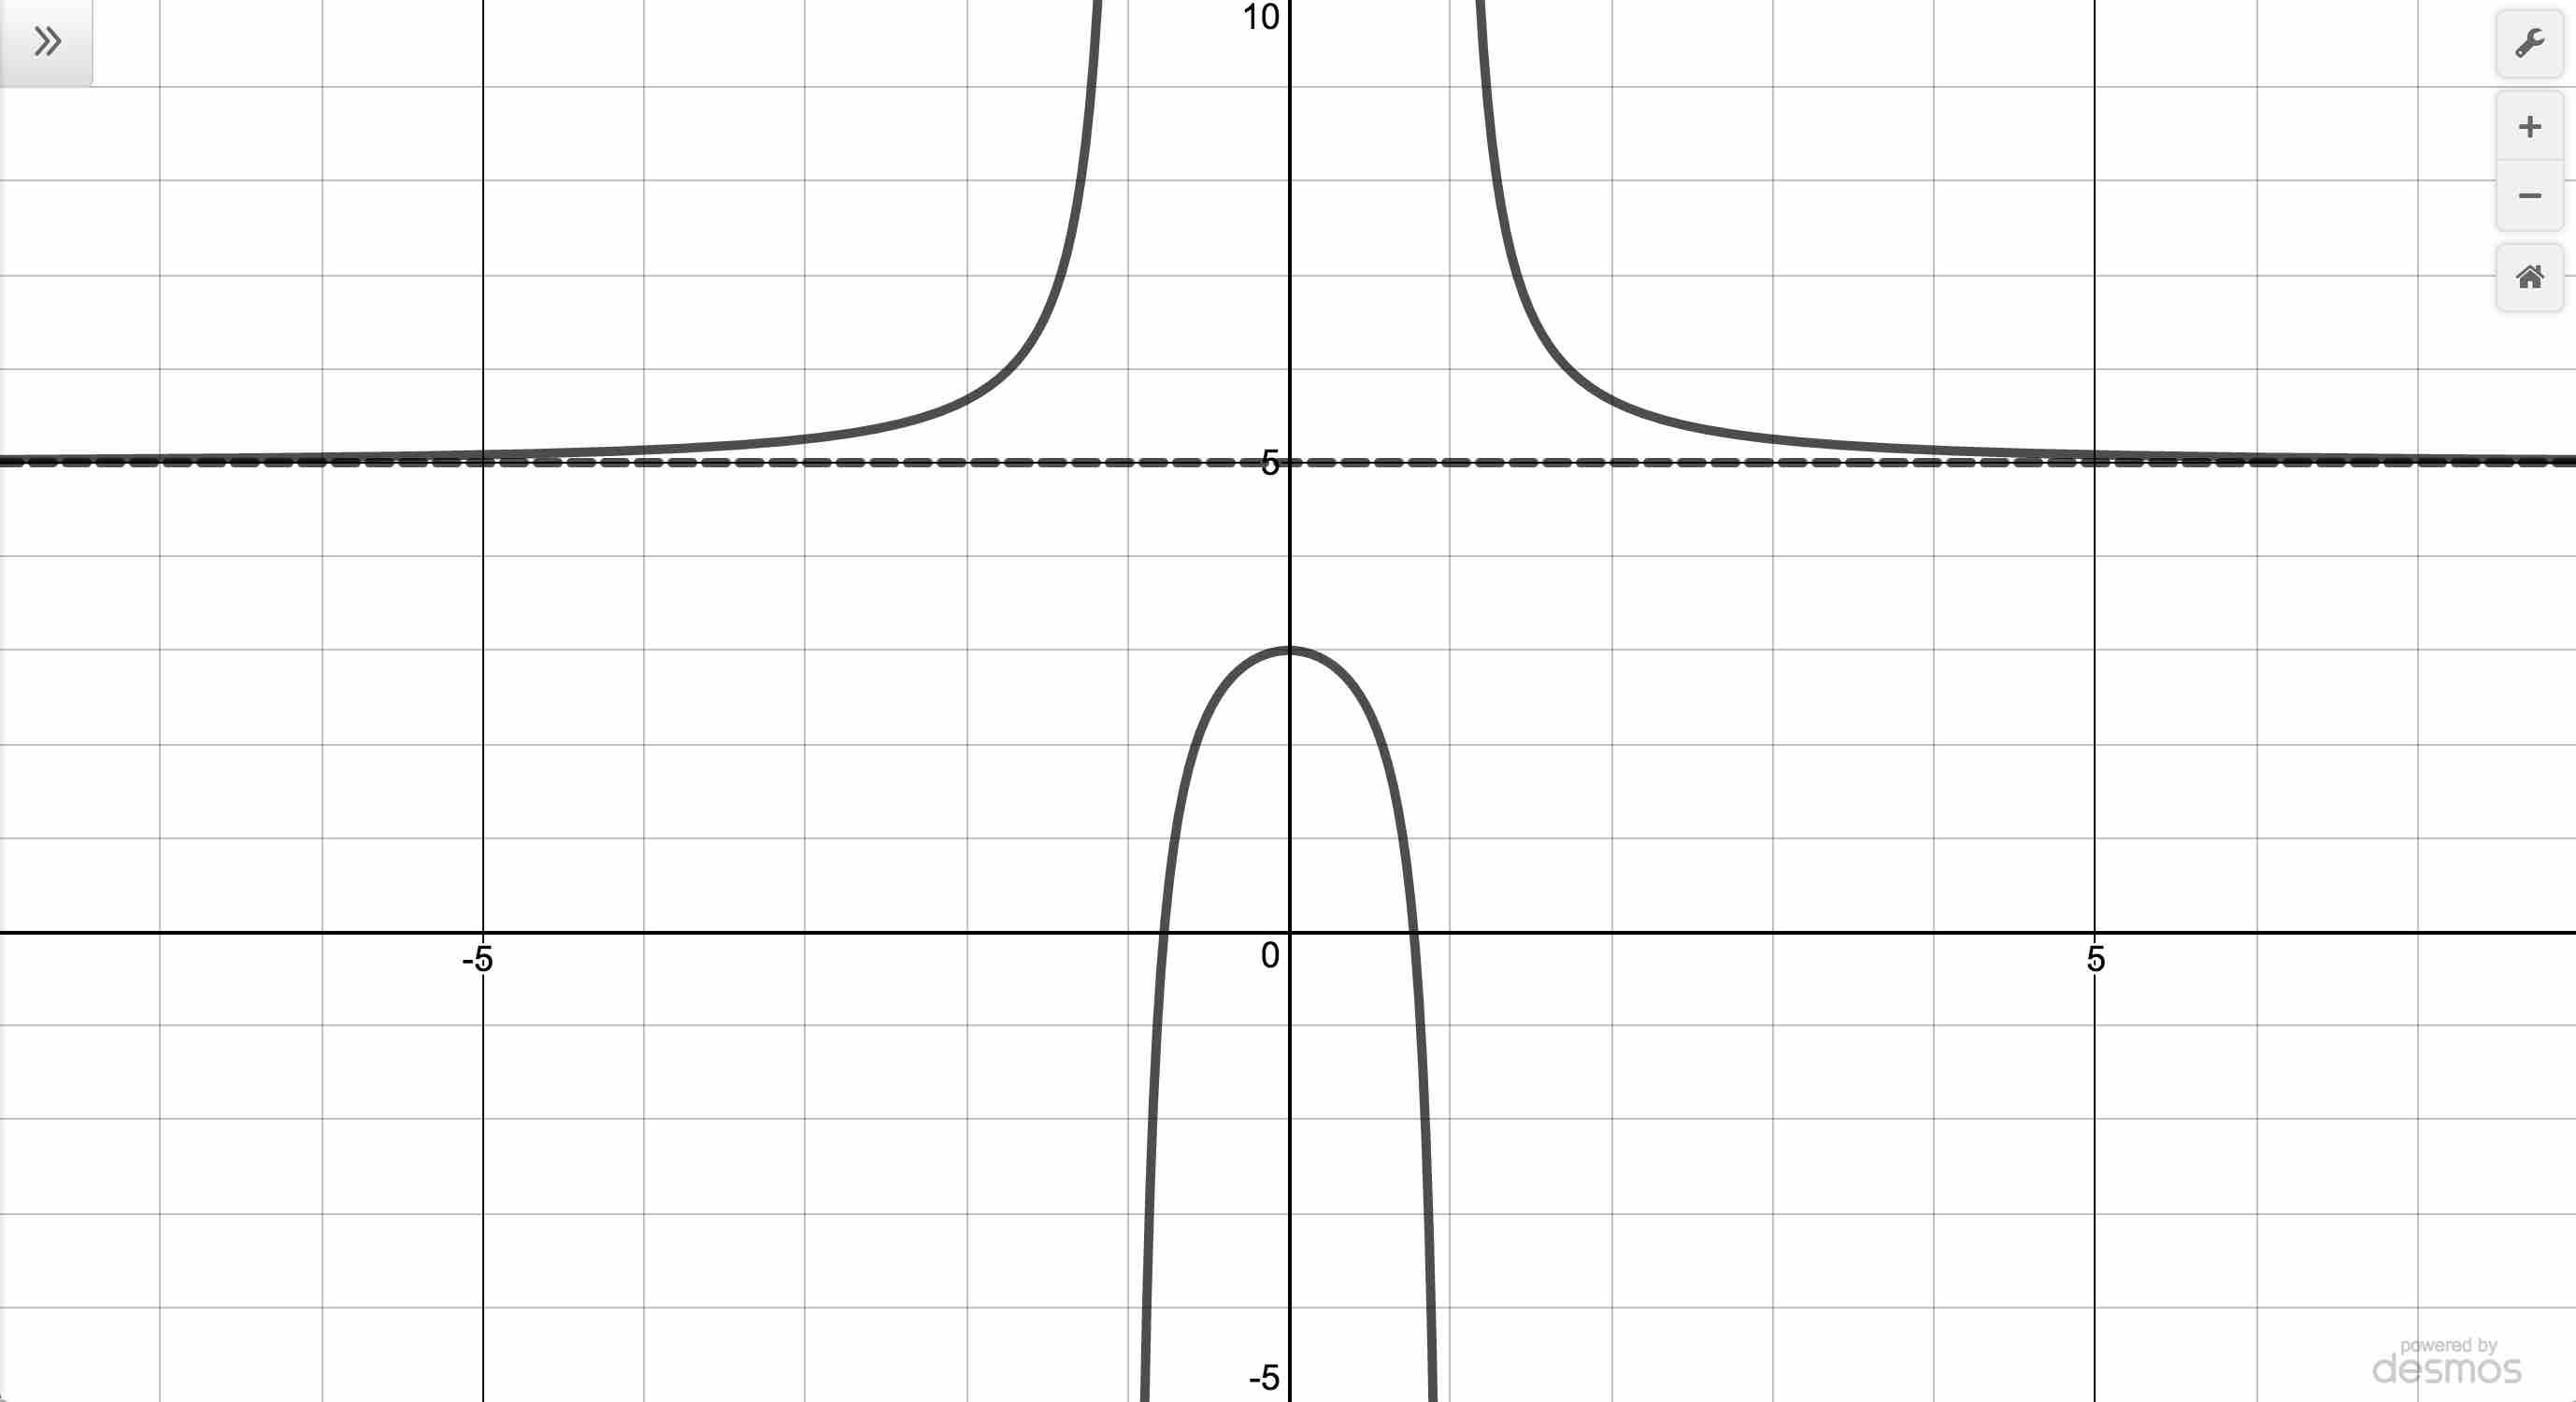
\includegraphics[width=3in]{./IntroRationalGraphics/HAEx04.jpg} \\
The graph of $y=h(t)$  & The graph of $y=r(x)$ \\


\end{tabular}
\end{center} 

\end{enumerate}

\qed

\end{ex}


We close this section with a discussion of the \textbf{third} (and final!) kind of asymptote which can be associated with the graphs of rational functions. Let us return to the function $g(x) = \frac{x^2-4}{x+1}$ in Example \ref{haexample}. Performing long division,\footnote{See the remarks following Theorem \ref{hathm}.} we get $g(x) = \frac{x^2-4}{x+1} = x-1 - \frac{3}{x+1}$.  Since the term $\frac{3}{x+1} \rightarrow 0$ as $x \rightarrow \pm \infty$, it stands to reason that as $x$ becomes unbounded, the function values   $g(x) = x-1 - \frac{3}{x+1} \approx x-1$.  Geometrically, this means that the graph of $y=g(x)$ should resemble the line $y = x-1$ as $x \rightarrow  -\infty$ and $x \rightarrow \infty$.  We see this play out both numerically and graphically below. (As usual, the asymptote $y = x-1$ is denoted by a dashed line.)

\begin{center}
\begin{tabular}{cc}

$\begin{array}{|r||c|c|}  \hline

  x & g(x) & x-1 \\ \hline
 -10 & \approx -10.6667 & -11 \\  \hline
 -100 & \approx -100.9697 & -101 \\  \hline 
 -1000 &  \approx -1000.9970&   -1001 \\ \hline 
  -10000 &  \approx -10000.9997 &  -10001 \\ \hline 
  \end{array} $ & 

$\begin{array}{|r||c|c|}  \hline

  x & g(x) & x-1 \\ \hline
 10 & \approx 8.7273 &    9 \\\hline
 100 & \approx 98.9703 &   99 \\ \hline 
 1000 &  \approx 998.9970 &  999 \\ \hline 
  10000 &  \approx 9998.9997 &   9999 \\ \hline 
  \end{array} $ \\
  
  \end{tabular}
  \end{center}
  
  
\begin{center}
   
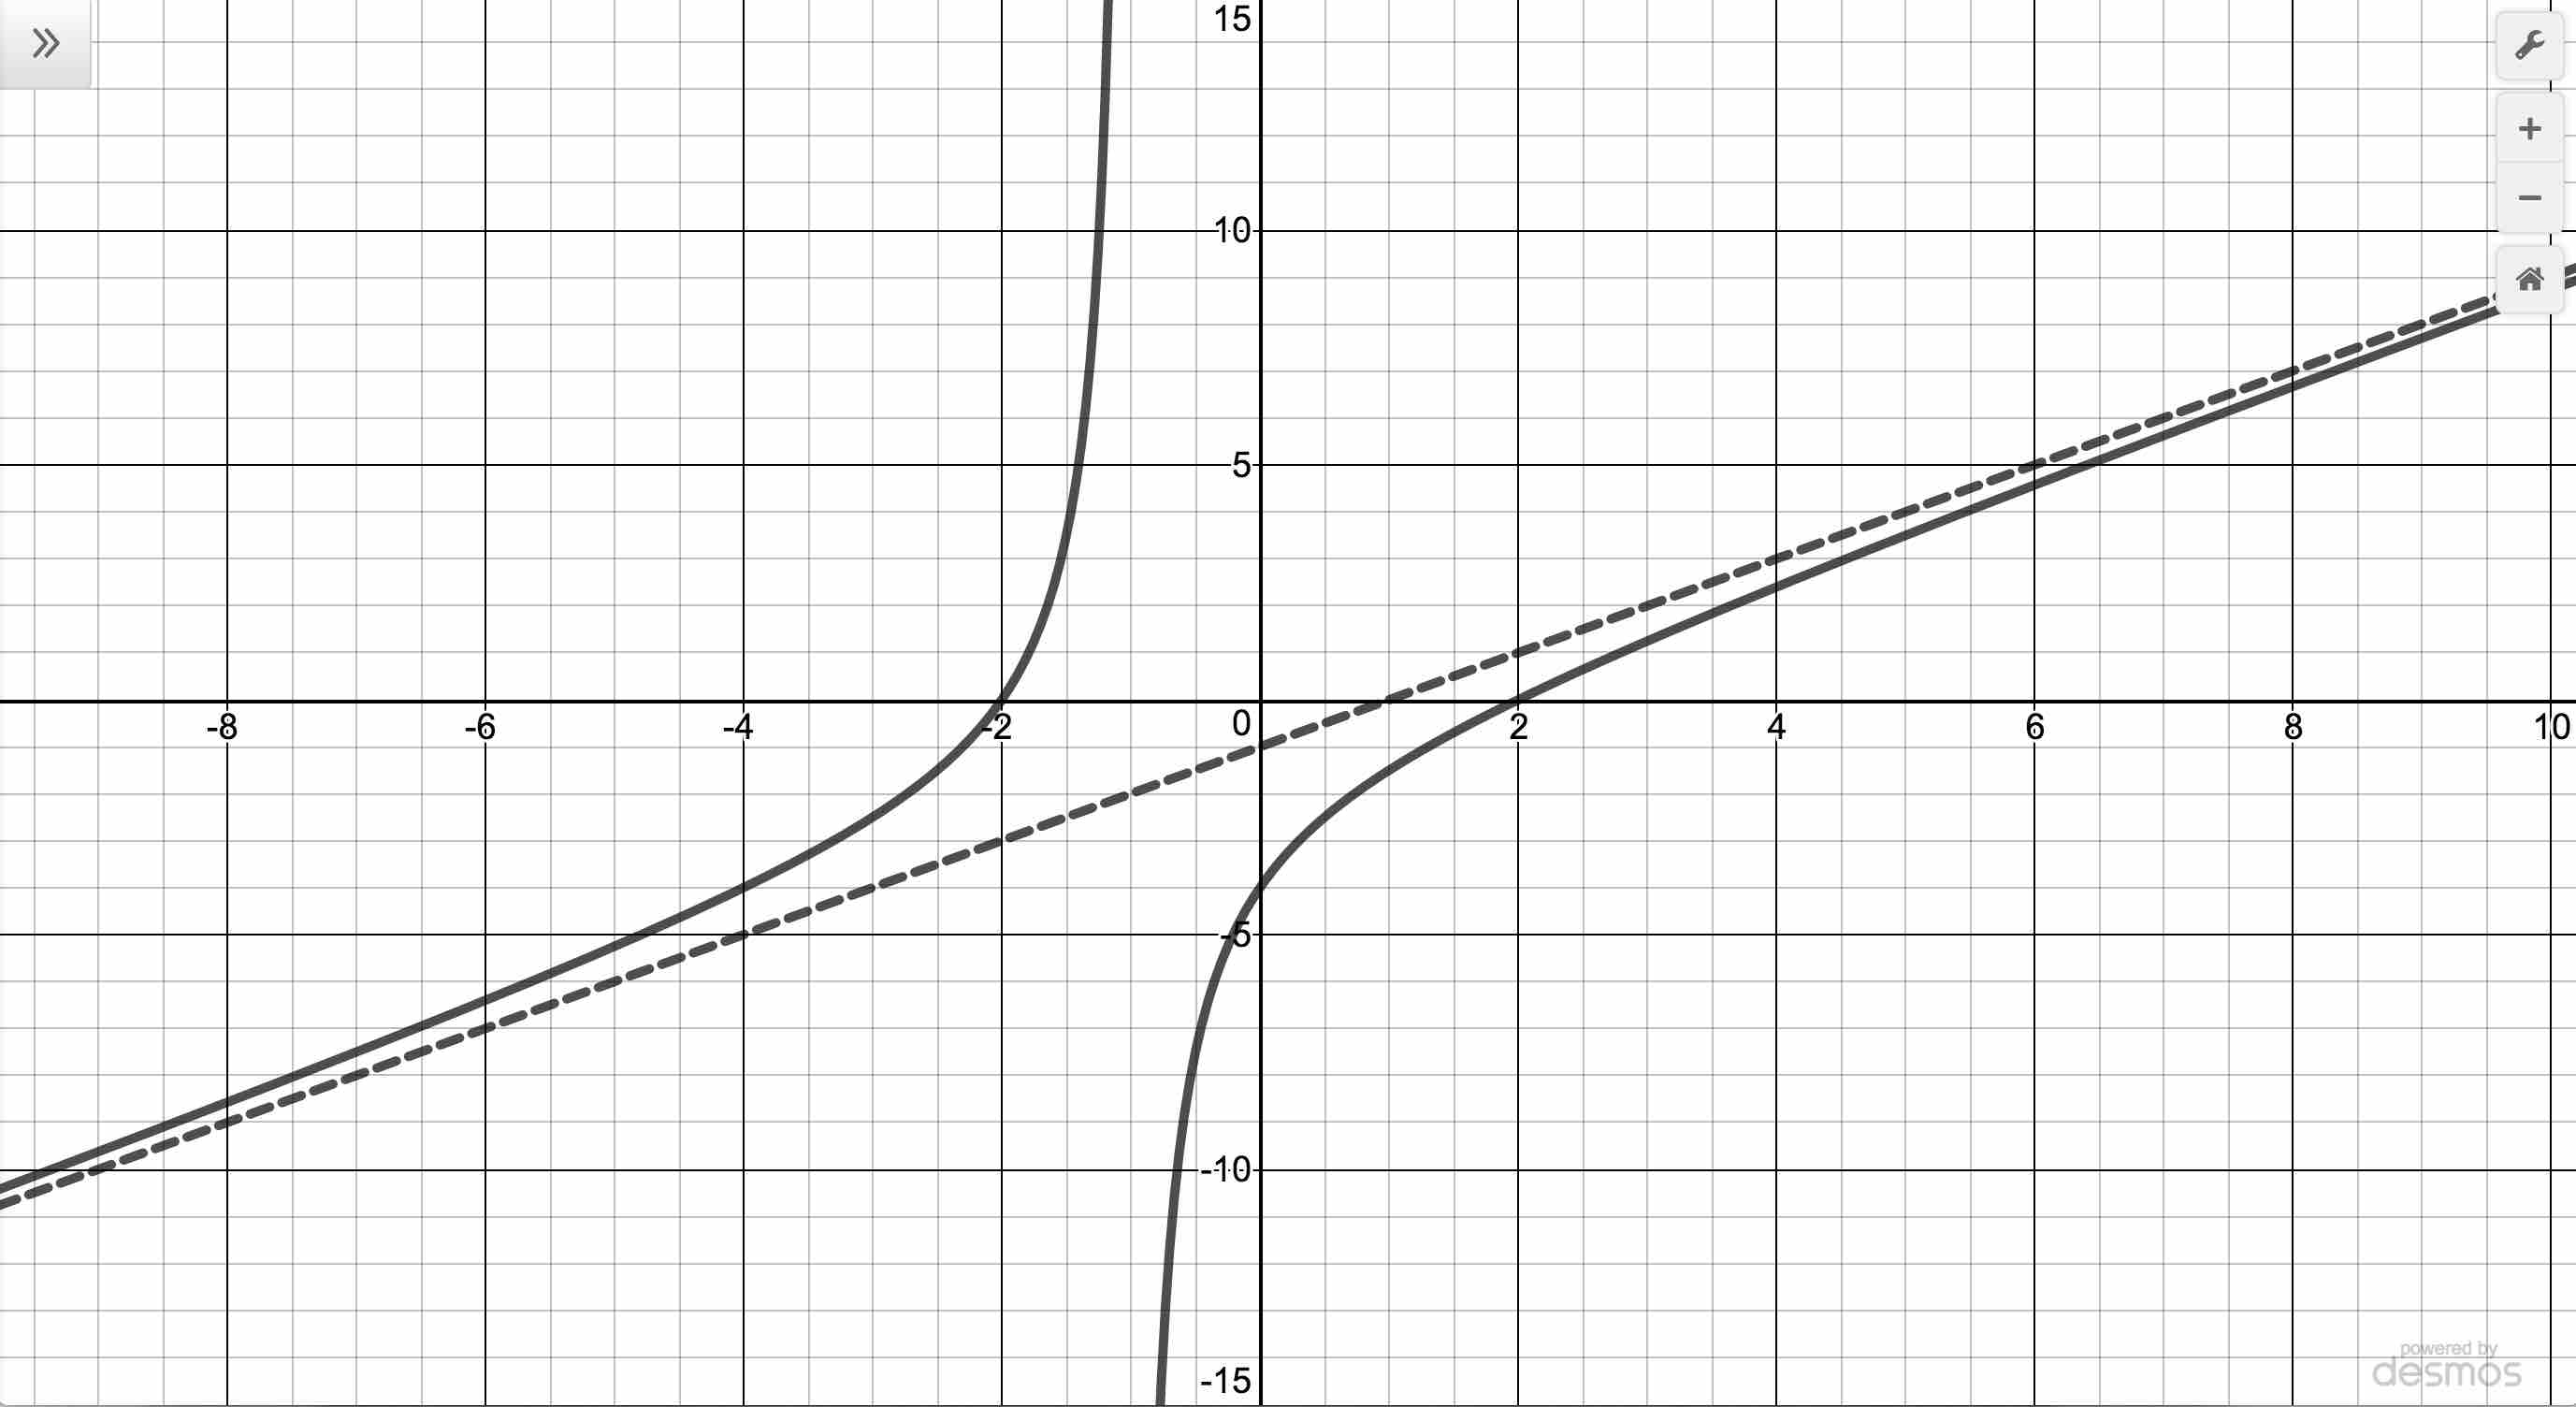
\includegraphics[width=4in]{./IntroRationalGraphics/SAEx01.jpg}

\end{center}
 
The way we symbolize the relationship between the end behavior of $y=g(x)$ with that of the line $y=x-1$ is to write `as $x \rightarrow  -\infty$ and $x \rightarrow \infty$, $g(x) \rightarrow x-1$' in order to have some notational consistency with what we have done earlier in this section when it comes to end behavior.\footnote{Other notations include $g(x) \asymp x-1$ or $g(x) \sim x-1$.}  In this case, we say the line $y=x-1$ is a \index{asymptote ! slant (oblique)} \index{slant asymptote} \index{oblique asymptote} \textbf{slant asymptote}\footnote{Also called an `oblique' asymptote in some, ostensibly higher class (and more expensive), texts.}  to the graph of $y=g(x)$.  Informally, the graph of a rational function has a slant asymptote if, as $x \rightarrow -\infty$ or as $x \rightarrow \infty$, the graph resembles a non-horizontal, or `slanted' line.  More formally, we define a slant asymptote as follows.


\medskip


\colorbox{ResultColor}{\bbm

\begin{defn} \label{sa} The line $y = mx+b$ where $m \neq 0$  is called a \index{asymptote ! slant ! formal definition of}\index{slant asymptote ! formal definition of}\textbf{slant asymptote} of the graph of a function $y=f(x)$ if as $x \rightarrow -\infty$ or as $x \rightarrow \infty$, $f(x)  \rightarrow mx+b$.


\end{defn}
\ebm}

\medskip


A few remarks are in order.  First, note that the stipulation $m \neq 0$ in Definition \ref{sa} is what makes the `slant' asymptote `slanted' as opposed to the case when $m=0$ in which case we'd have a horizontal asymptote.  

Secondly, while we have motivated what me mean intuitively by the notation `$f(x)  \rightarrow mx+b$,' like so many ideas in this section, the formal definition requires Calculus.  Another way to express this sentiment, however, is to rephrase `$f(x)  \rightarrow mx+b$' as `$[f(x) - (mx+b)] \rightarrow 0$.'  In other words, the graph of $y=f(x)$ has the \textbf{slant} asymptote $y = mx+b$ if and only if the graph of $y = f(x) - (mx+b)$ has a \textbf{horizontal} asymptote $y=0$.   This last sentiment can be encoded using limit notation as follows.

\medskip


\colorbox{ResultColor}{\bbm

\begin{defn} \label{sareprise} The line $y = mx+b$ where $m \neq 0$  is called a \index{asymptote ! slant ! formal definition of}\index{slant asymptote ! formal definition of}\textbf{slant asymptote} of the graph of a function $y=f(x)$ if either $\ds{\lim_{x \rightarrow -\infty} [f(x) - (mx+b)] = 0}$ or $\ds{\lim_{x \rightarrow \infty} [f(x) - (mx+b)] = 0}$ (or both!).

\end{defn}
\ebm}

\medskip


Our next task is to determine the conditions under which the graph of a rational function has a slant asymptote, and if it does, how to find it.  In the case of $g(x) = \frac{x^2-4}{x+1}$, the degree of the numerator $x^2-4$ is $2$, which is \textbf{exactly one more} than the degree if its denominator $x+1$ which is $1$.  This results in a \textbf{linear} quotient polynomial, and it is this quotient polynomial which is the slant asymptote.  Generalizing this situation gives us the following theorem.\footnote{Once again, this theorem is brought to you courtesy of Theorem \ref{Polydivision} and Calculus.}

\medskip

\colorbox{ResultColor}{\bbm

\begin{thm} \textbf{Determination of Slant Asymptotes:} \label{sathm} Suppose $r$ is a rational function and $r(x) = \frac{p(x)}{q(x)}$, where the degree of $p$ is \textbf{exactly} one more than the degree of $q$.  Then the graph of $y=r(x)$ has \index{asymptote ! slant ! determination of}\index{slant asymptote ! determination of} the slant asymptote $y=L(x)$ where $L(x)$ is the quotient obtained by dividing $p(x)$ by $q(x)$.

\end{thm}
\ebm}

\medskip

In the same way that Theorem \ref{hathm} gives us an easy way to see if the graph of a rational function $r(x) = \frac{p(x)}{q(x)}$ has a horizontal asymptote by comparing the degrees of the numerator and denominator, Theorem \ref{sathm} gives us an easy way to check for slant asymptotes.  Unlike Theorem \ref{hathm}, which gives us a quick way to \textbf{find} the horizontal asymptotes (if any exist), Theorem \ref{sathm} gives us no such `short-cut'.  If a slant asymptote exists, we have no recourse but to use long division to find it.\footnote{That's OK, though.  In the next section, we'll use long division to analyze end behavior and it's worth the effort!}  

\begin{ex} \label{saexample}  For each of the following functions:

\begin{itemize}

\item find the slant asymptote, if it exists.

\item  verify your answer using a graphing utility.

\item  investigate any apparent symmetry of the graph about the $y$-axis or origin.

\end{itemize}


\begin{multicols}{2}
\begin{enumerate}

\item  $f(x) = \dfrac{x^2-4x+2}{1-x}$  

\item  \label{sacancel} $g(t) = \dfrac{t^2-4}{t-2}$

\setcounter{HW}{\value{enumi}}
\end{enumerate}
\end{multicols}

\begin{multicols}{2}
\begin{enumerate}
\setcounter{enumi}{\value{HW}}


\item  $h(x) = \dfrac{x^3+1}{x^2-4}$

\item  $r(t) = 2t-1+\dfrac{4t^3}{1-t^2}$ \vphantom{$h(x) = \dfrac{x^3+1}{x^2-4}$}

\setcounter{HW}{\value{enumi}}
\end{enumerate}
\end{multicols}



{\bf Solution.}

\begin{enumerate}

\item  The degree of the numerator is $2$ and the degree of the denominator is $1$, so Theorem \ref{sathm} guarantees us a slant asymptote.  To find it, we divide $1-x = -x+1$ into $x^2-4x+2$ and get a quotient of $-x+3$, so our slant asymptote is $y=-x+3$.  We confirm this graphically below.

\item  As with the previous example, the degree of the numerator $g(t) = \frac{t^2-4}{t-2}$ is $2$ and the degree of the denominator is $1$, so Theorem \ref{sathm} applies.  In this case, 

\[ g(t) = \frac{t^2-4}{t-2} = \frac{(t+2)(t-2)}{(t-2)} = \frac{(t+2) \cancel{(t-2)}}{\cancelto{1}{(t-2)}} = t+2, \quad t \neq 2\]

so we have that the slant asymptote $y=t+2$ is identical to the graph of $y=g(t)$ except at $t=2$ (where the latter has a `hole' at $(2,4)$.) While the word `asymptote' has the connotation of `approaching but not equaling,' Definitions \ref{ha} and  \ref{sa} allow for these extreme cases.

\begin{center}
\begin{tabular}{cc}

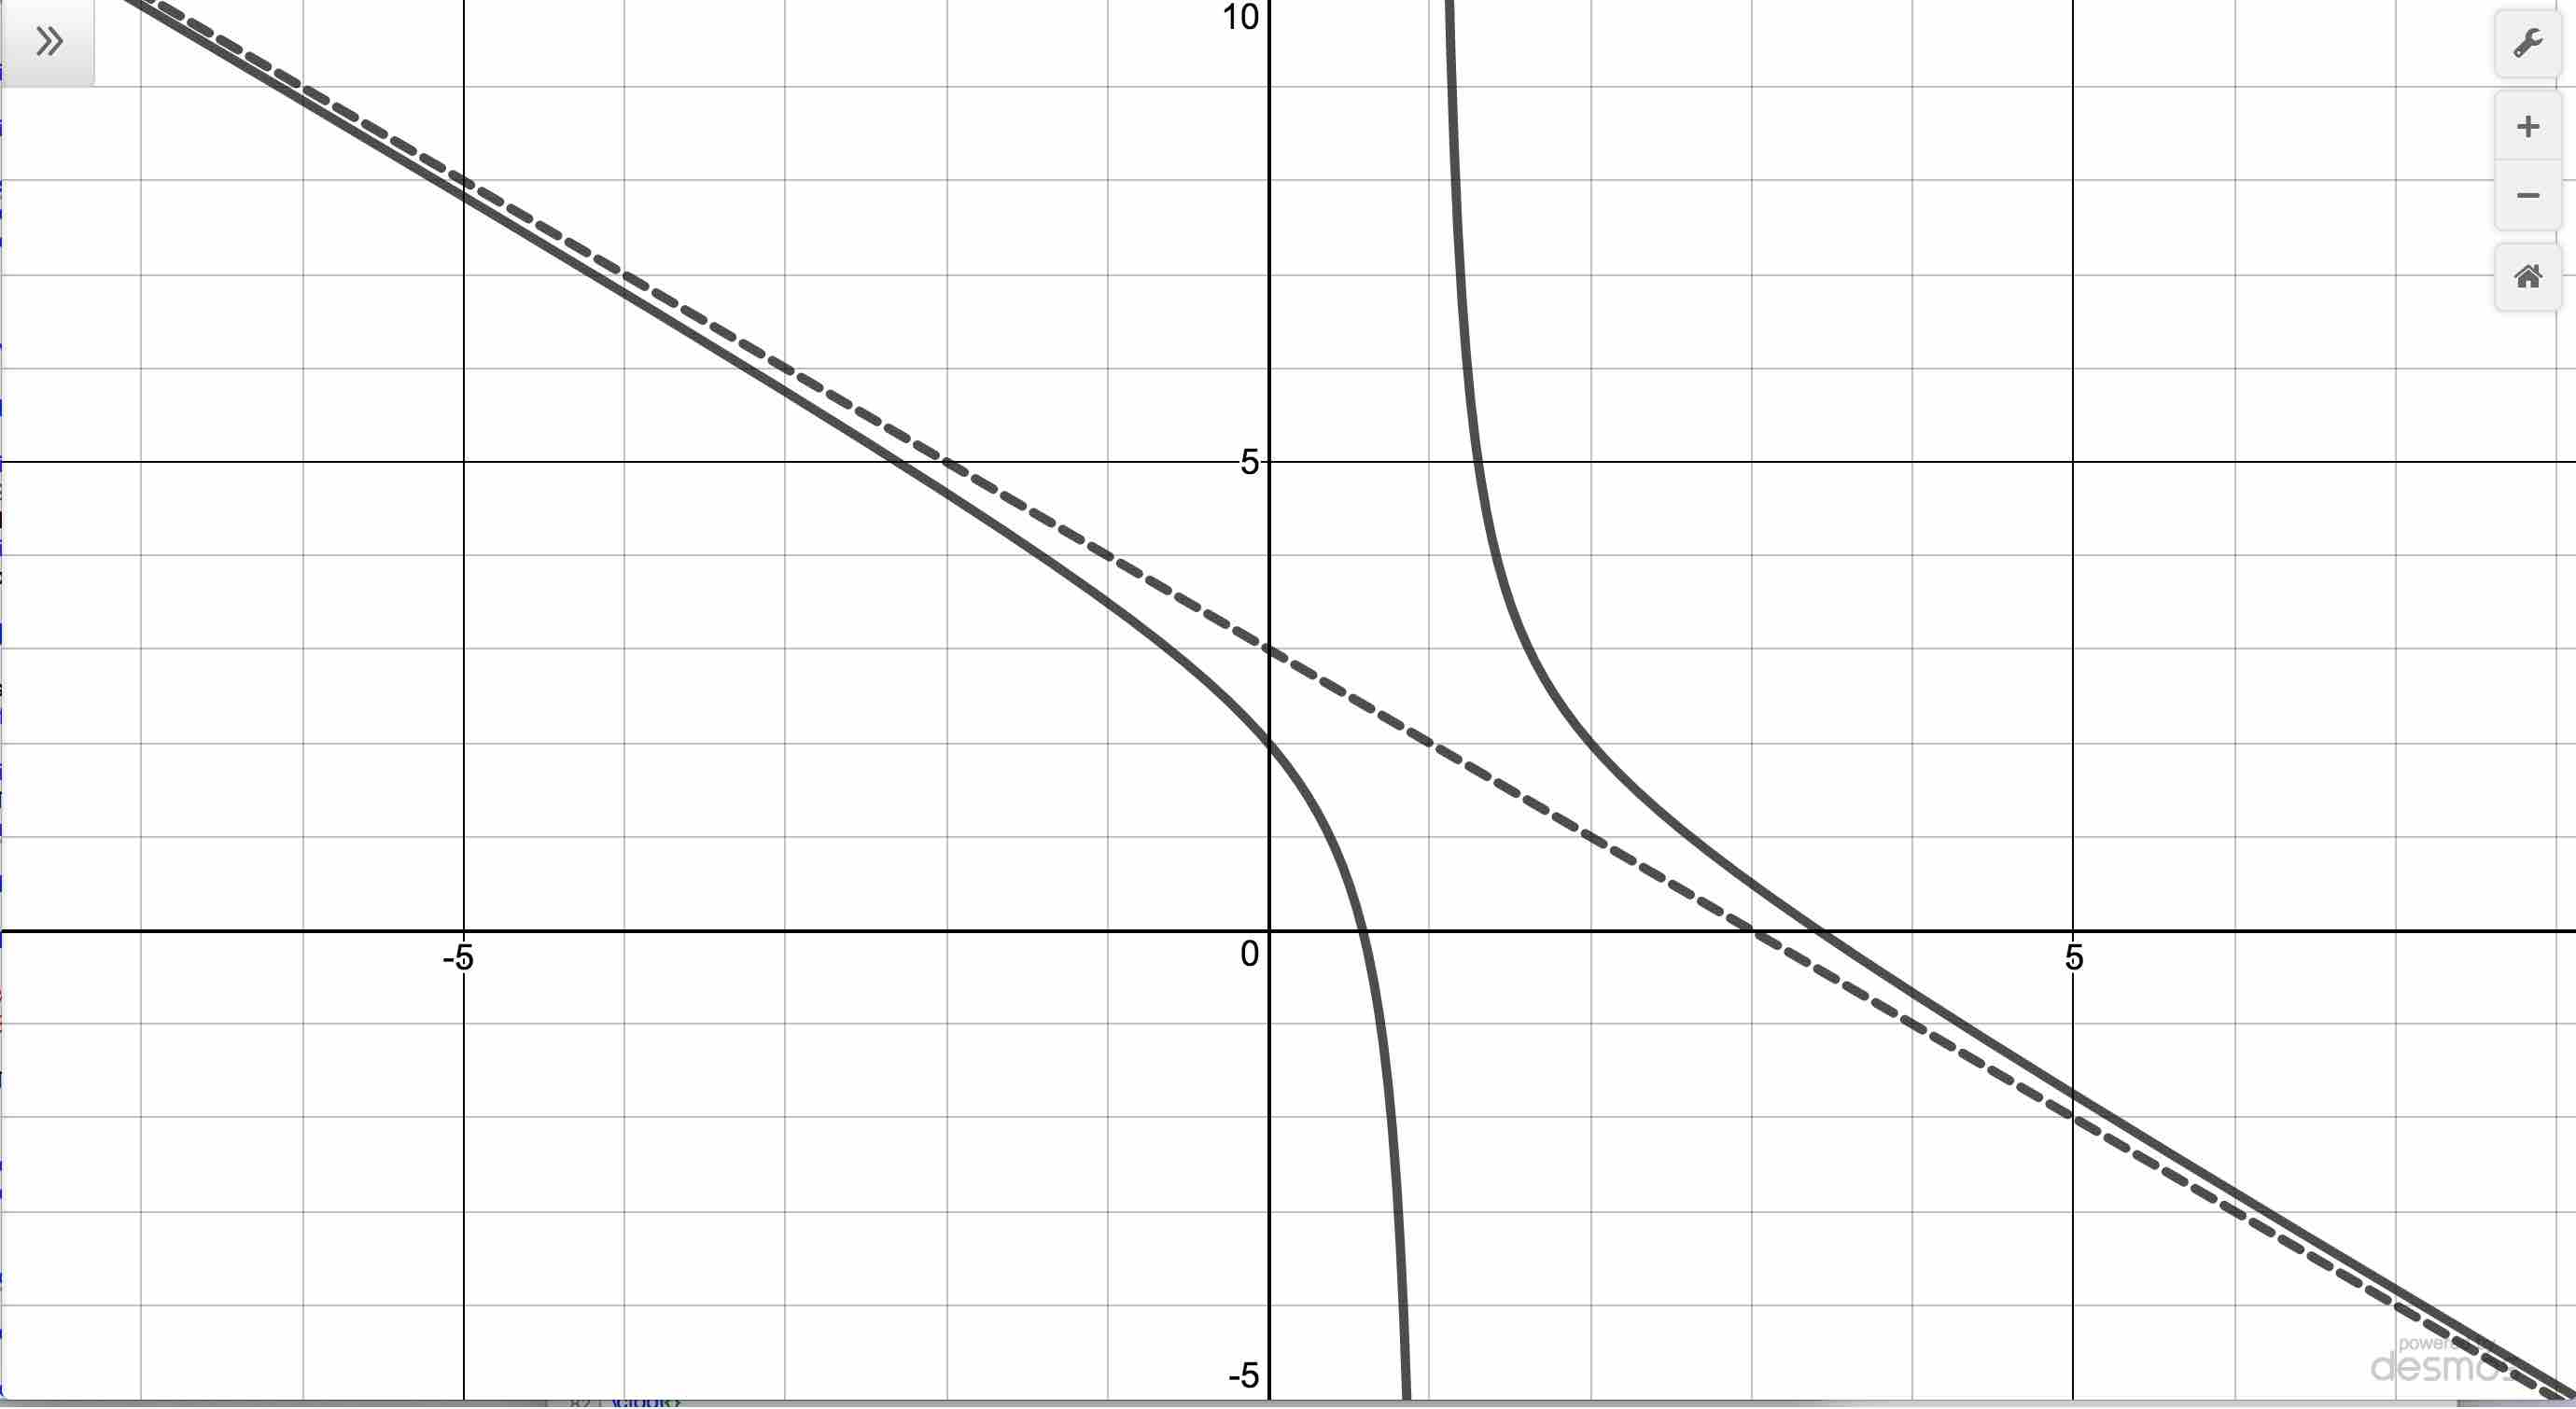
\includegraphics[width=3in]{./IntroRationalGraphics/SAEx02.jpg}  & 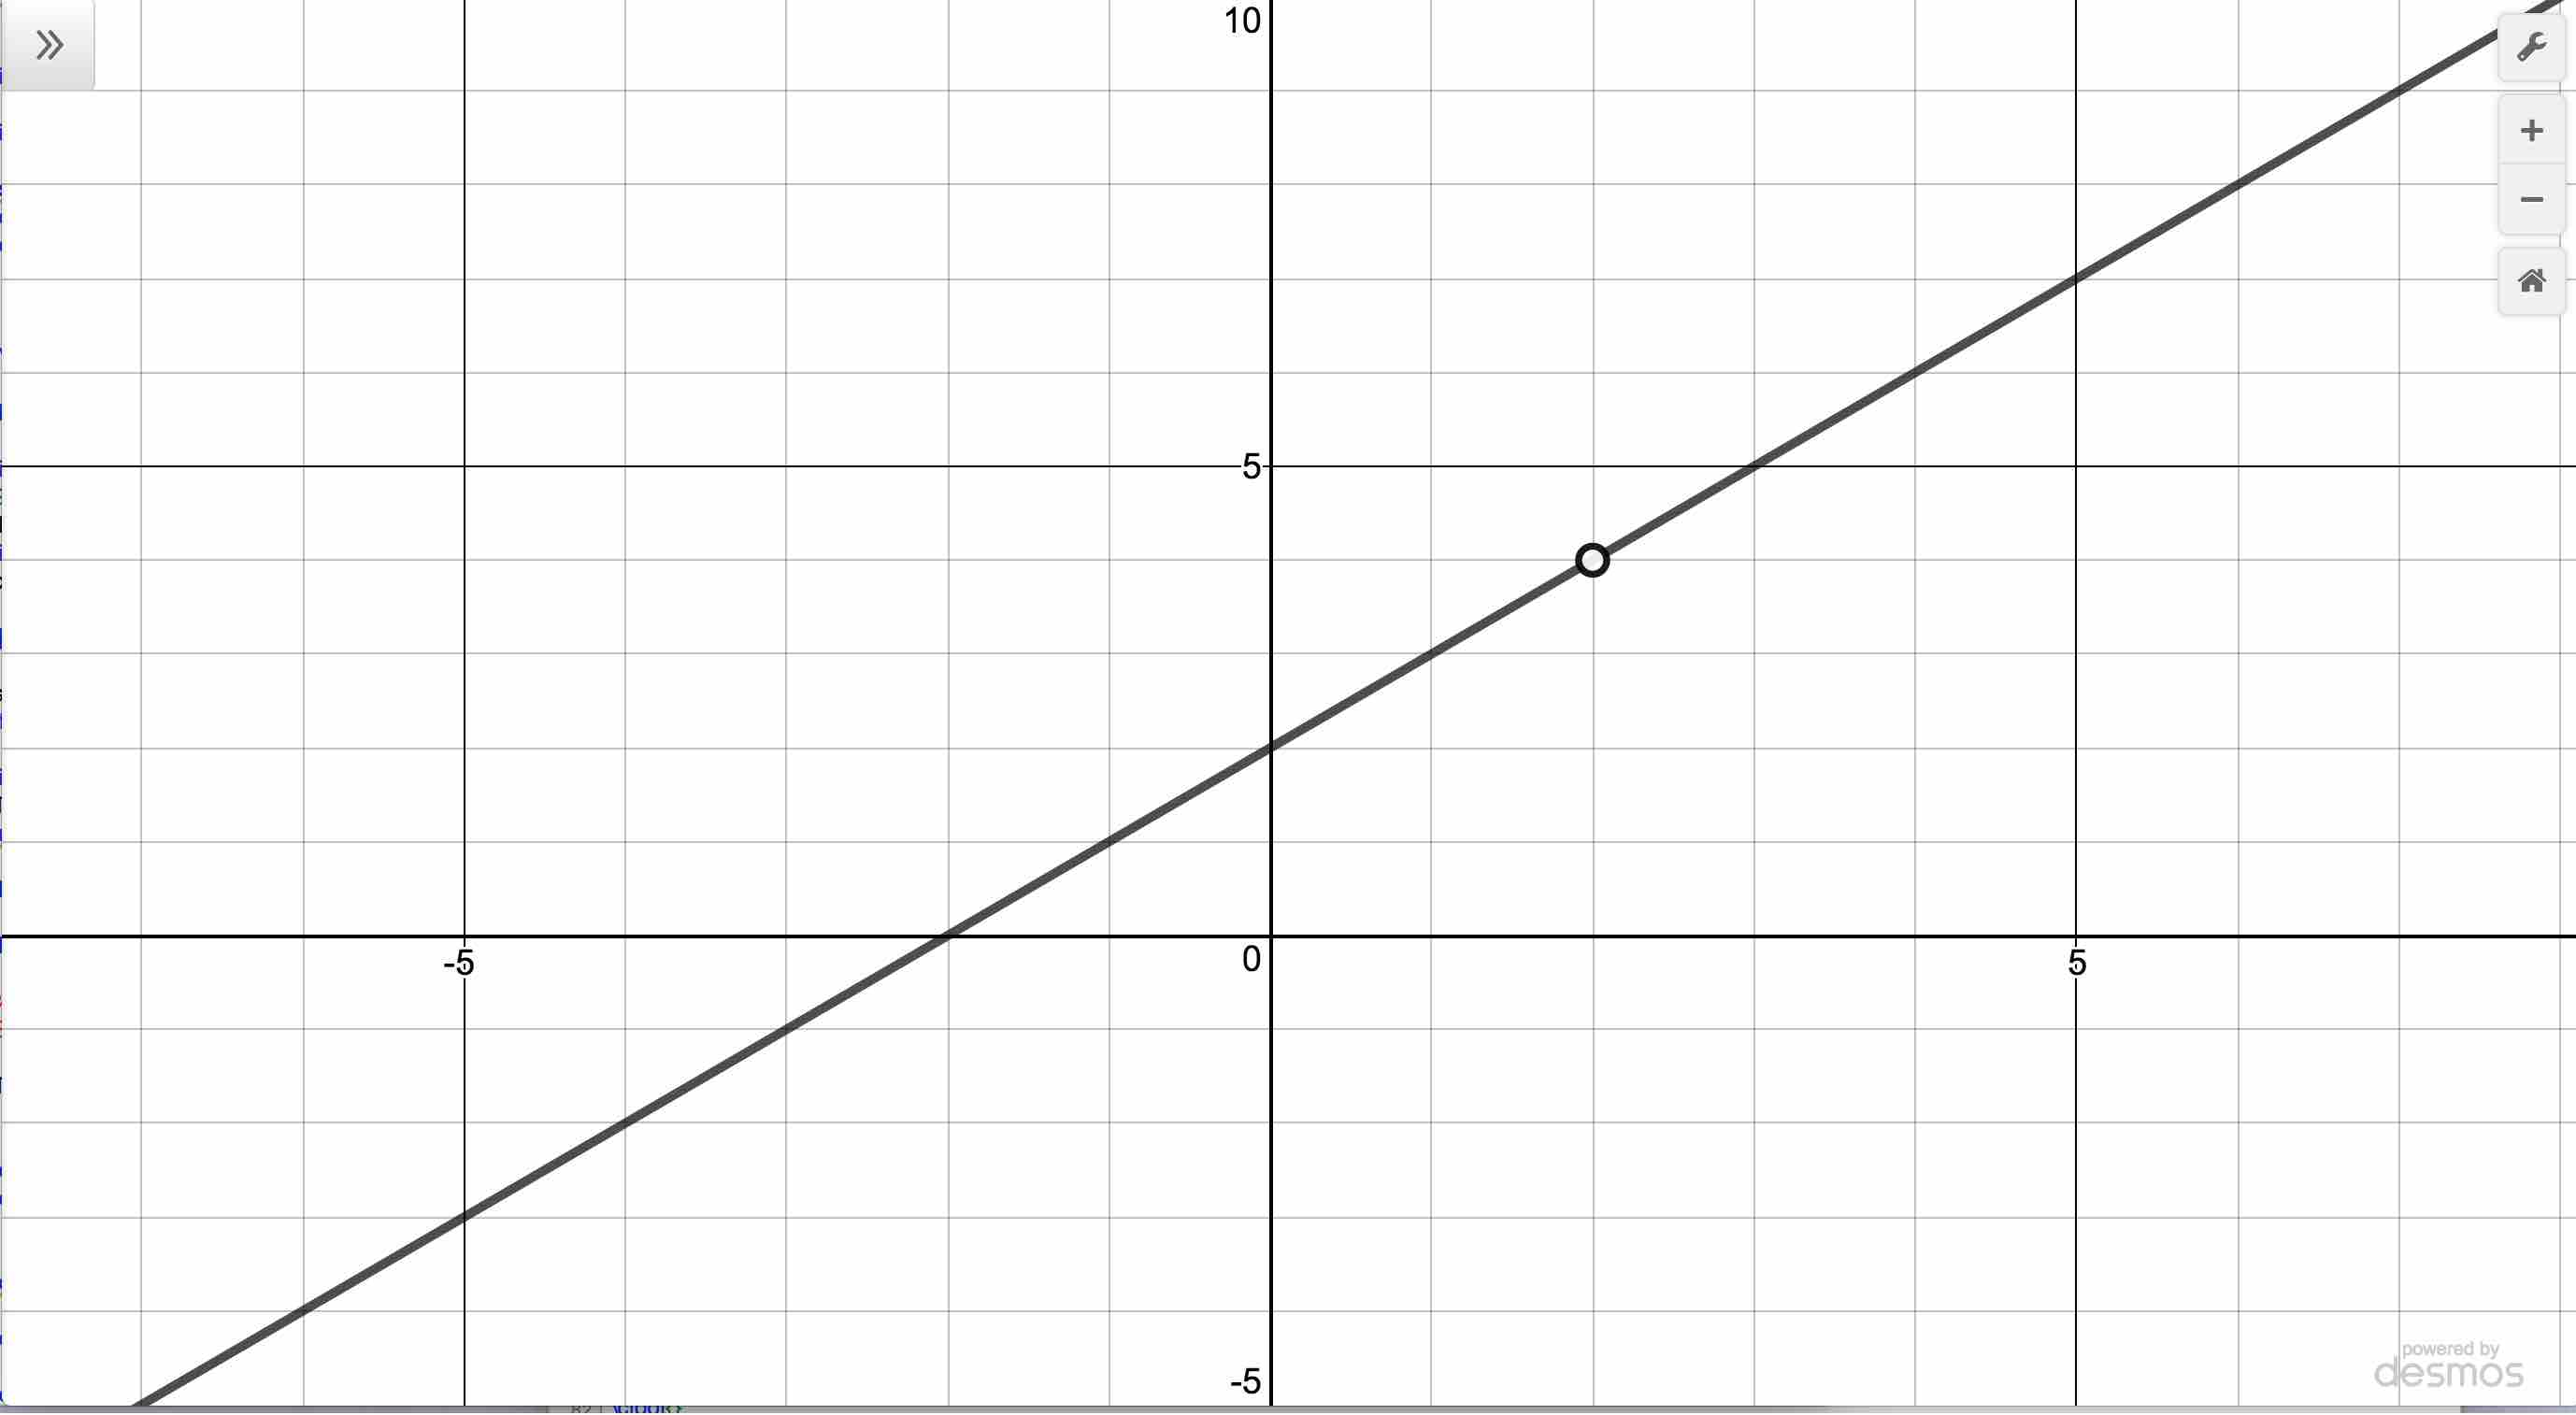
\includegraphics[width=3in]{./IntroRationalGraphics/SAEx03.jpg} \\
The graph of $y=f(x)$  & The graph of $y=g(t)$ \\


\end{tabular}
\end{center} 

\item   For $h(x) = \frac{x^3+1}{x^2-4}$, the degree of the numerator is $3$ and the degree of the denominator is $2$ so again, we are guaranteed the existence of a slant asymptote.  The long division $\left(x^3+1 \right) \div \left(x^2-4\right)$ gives a quotient of just $x$, so our slant asymptote is the line $y=x$.  The graphing utility confirms this.  

Note the graph of $h$ appears to be symmetric about the origin.  We check $h(-x) = \frac{(-x)^3+1}{(-x)^2-4} = \frac{-x^3+1}{x^2-4} = - \frac{x^3-1}{x^2-4}$.  However, $-h(x) = - \frac{x^3+1}{x^2-4}$, so it appears as if $h(-x) \neq -h(x)$ for all $x$.  Checking $x=1$, we find $h(1) = -\frac{2}{3}$ but $h(-1) = 0$ which shows the graph of $h$, is in fact,  \textbf{not} symmetric about the origin.

\item  For our last example,  $r(t) = 2t-1+\frac{4t^3}{1-t^2}$, the expression $r(t)$ is not in the form to apply Theorem \ref{sathm} directly.  We can, nevertheless, appeal to the spirit of the theorem and use long division to rewrite the term $\frac{4t^3}{1-t^2} = -4t + \frac{4t}{1-t^2}$.  We then get:

 \[ \begin{array}{rcl}
 
 r(t) & = & 2t-1+\dfrac{4t^3}{1-t^2} \\
       &= &  2t-1-4t+\dfrac{4t}{1-t^2} \\
       & = & -2t-1 + \dfrac{4t}{1-t^2} \\ \end{array}\]
       
As $t \rightarrow -\infty$ or $x \rightarrow \infty$,  Theorem \ref{EBPolynomials} gives  $\frac{4t}{1-t^2} \approx \frac{4t}{-t^2} = -\frac{4}{t} \rightarrow 0$.  Hence, as $t \rightarrow -\infty$ or $t \rightarrow \infty$, $r(t) \rightarrow -2t-1$, so $y = -2t-1$ is the slant asymptote to the graph as confirmed by the graphing utility below.  From a distance, the graph of $r$ appears to be symmetric about the origin.  However, if we look carefully, we see the $y$-intercept is $(0,-1)$, as borne out by the computation $r(0) = -1$.  Hence $r$ cannot be odd.\footnote{Do you see why?}

\begin{center}
\begin{tabular}{cc}

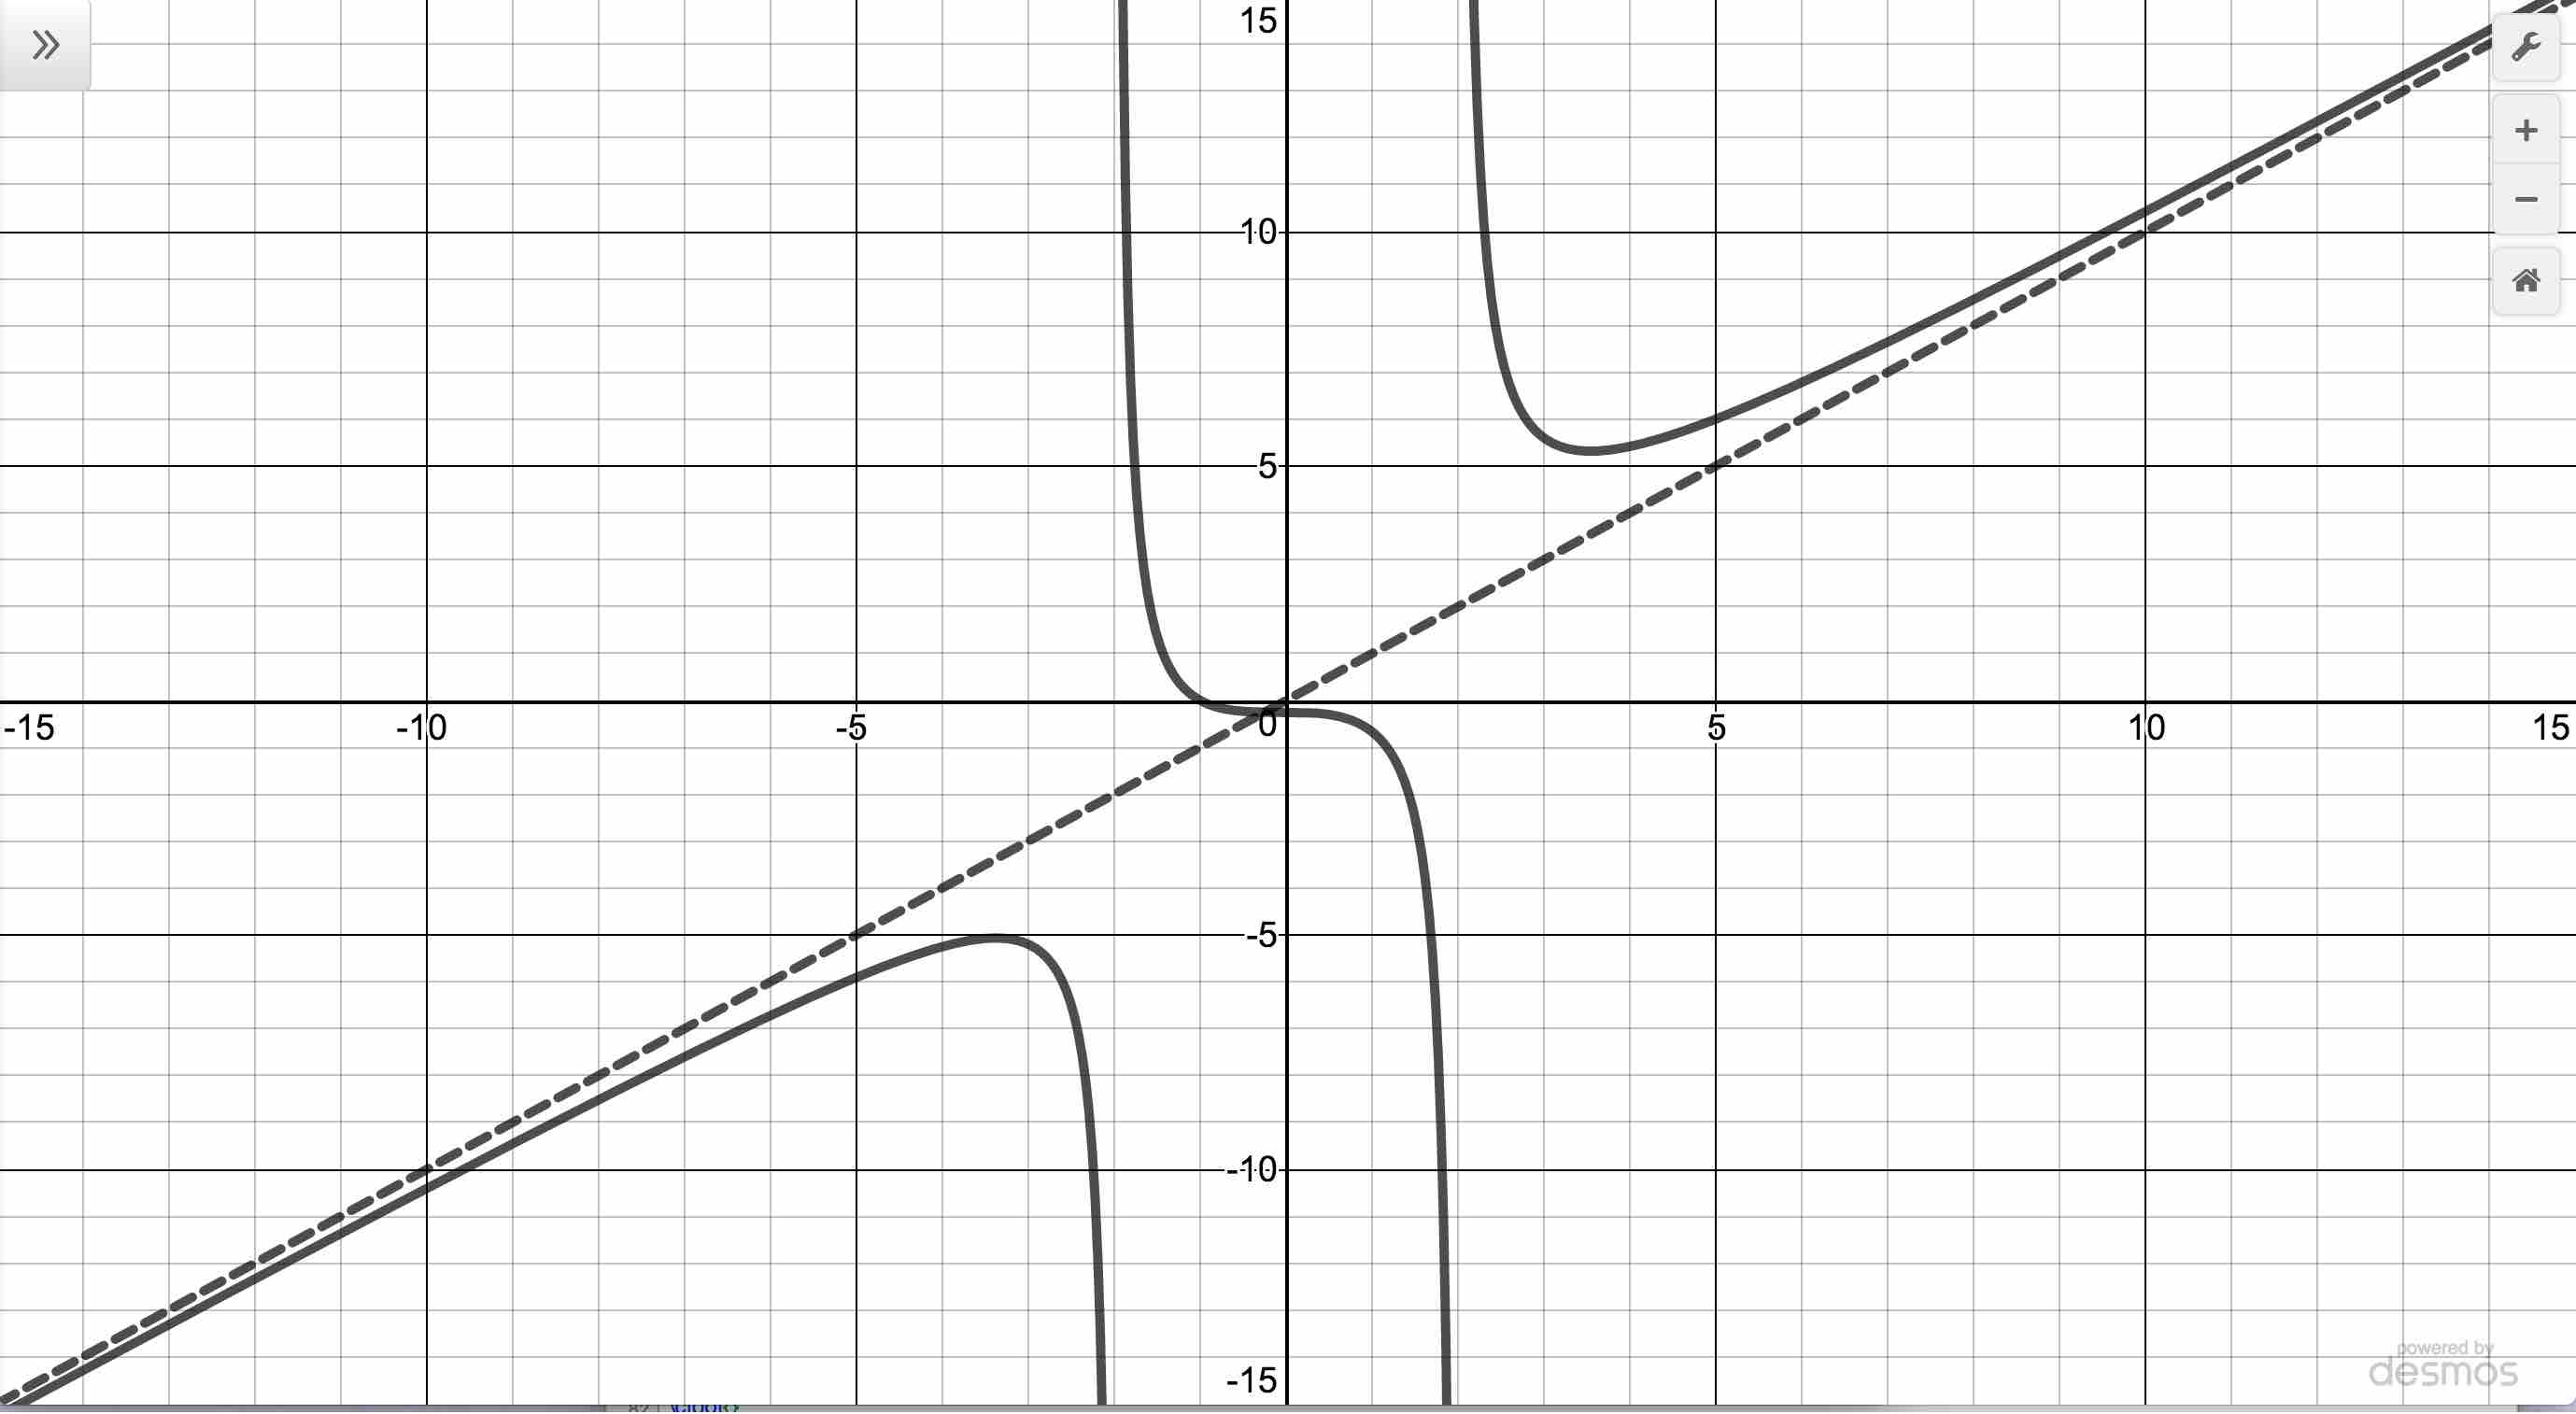
\includegraphics[width=3in]{./IntroRationalGraphics/SAEx04.jpg}  & 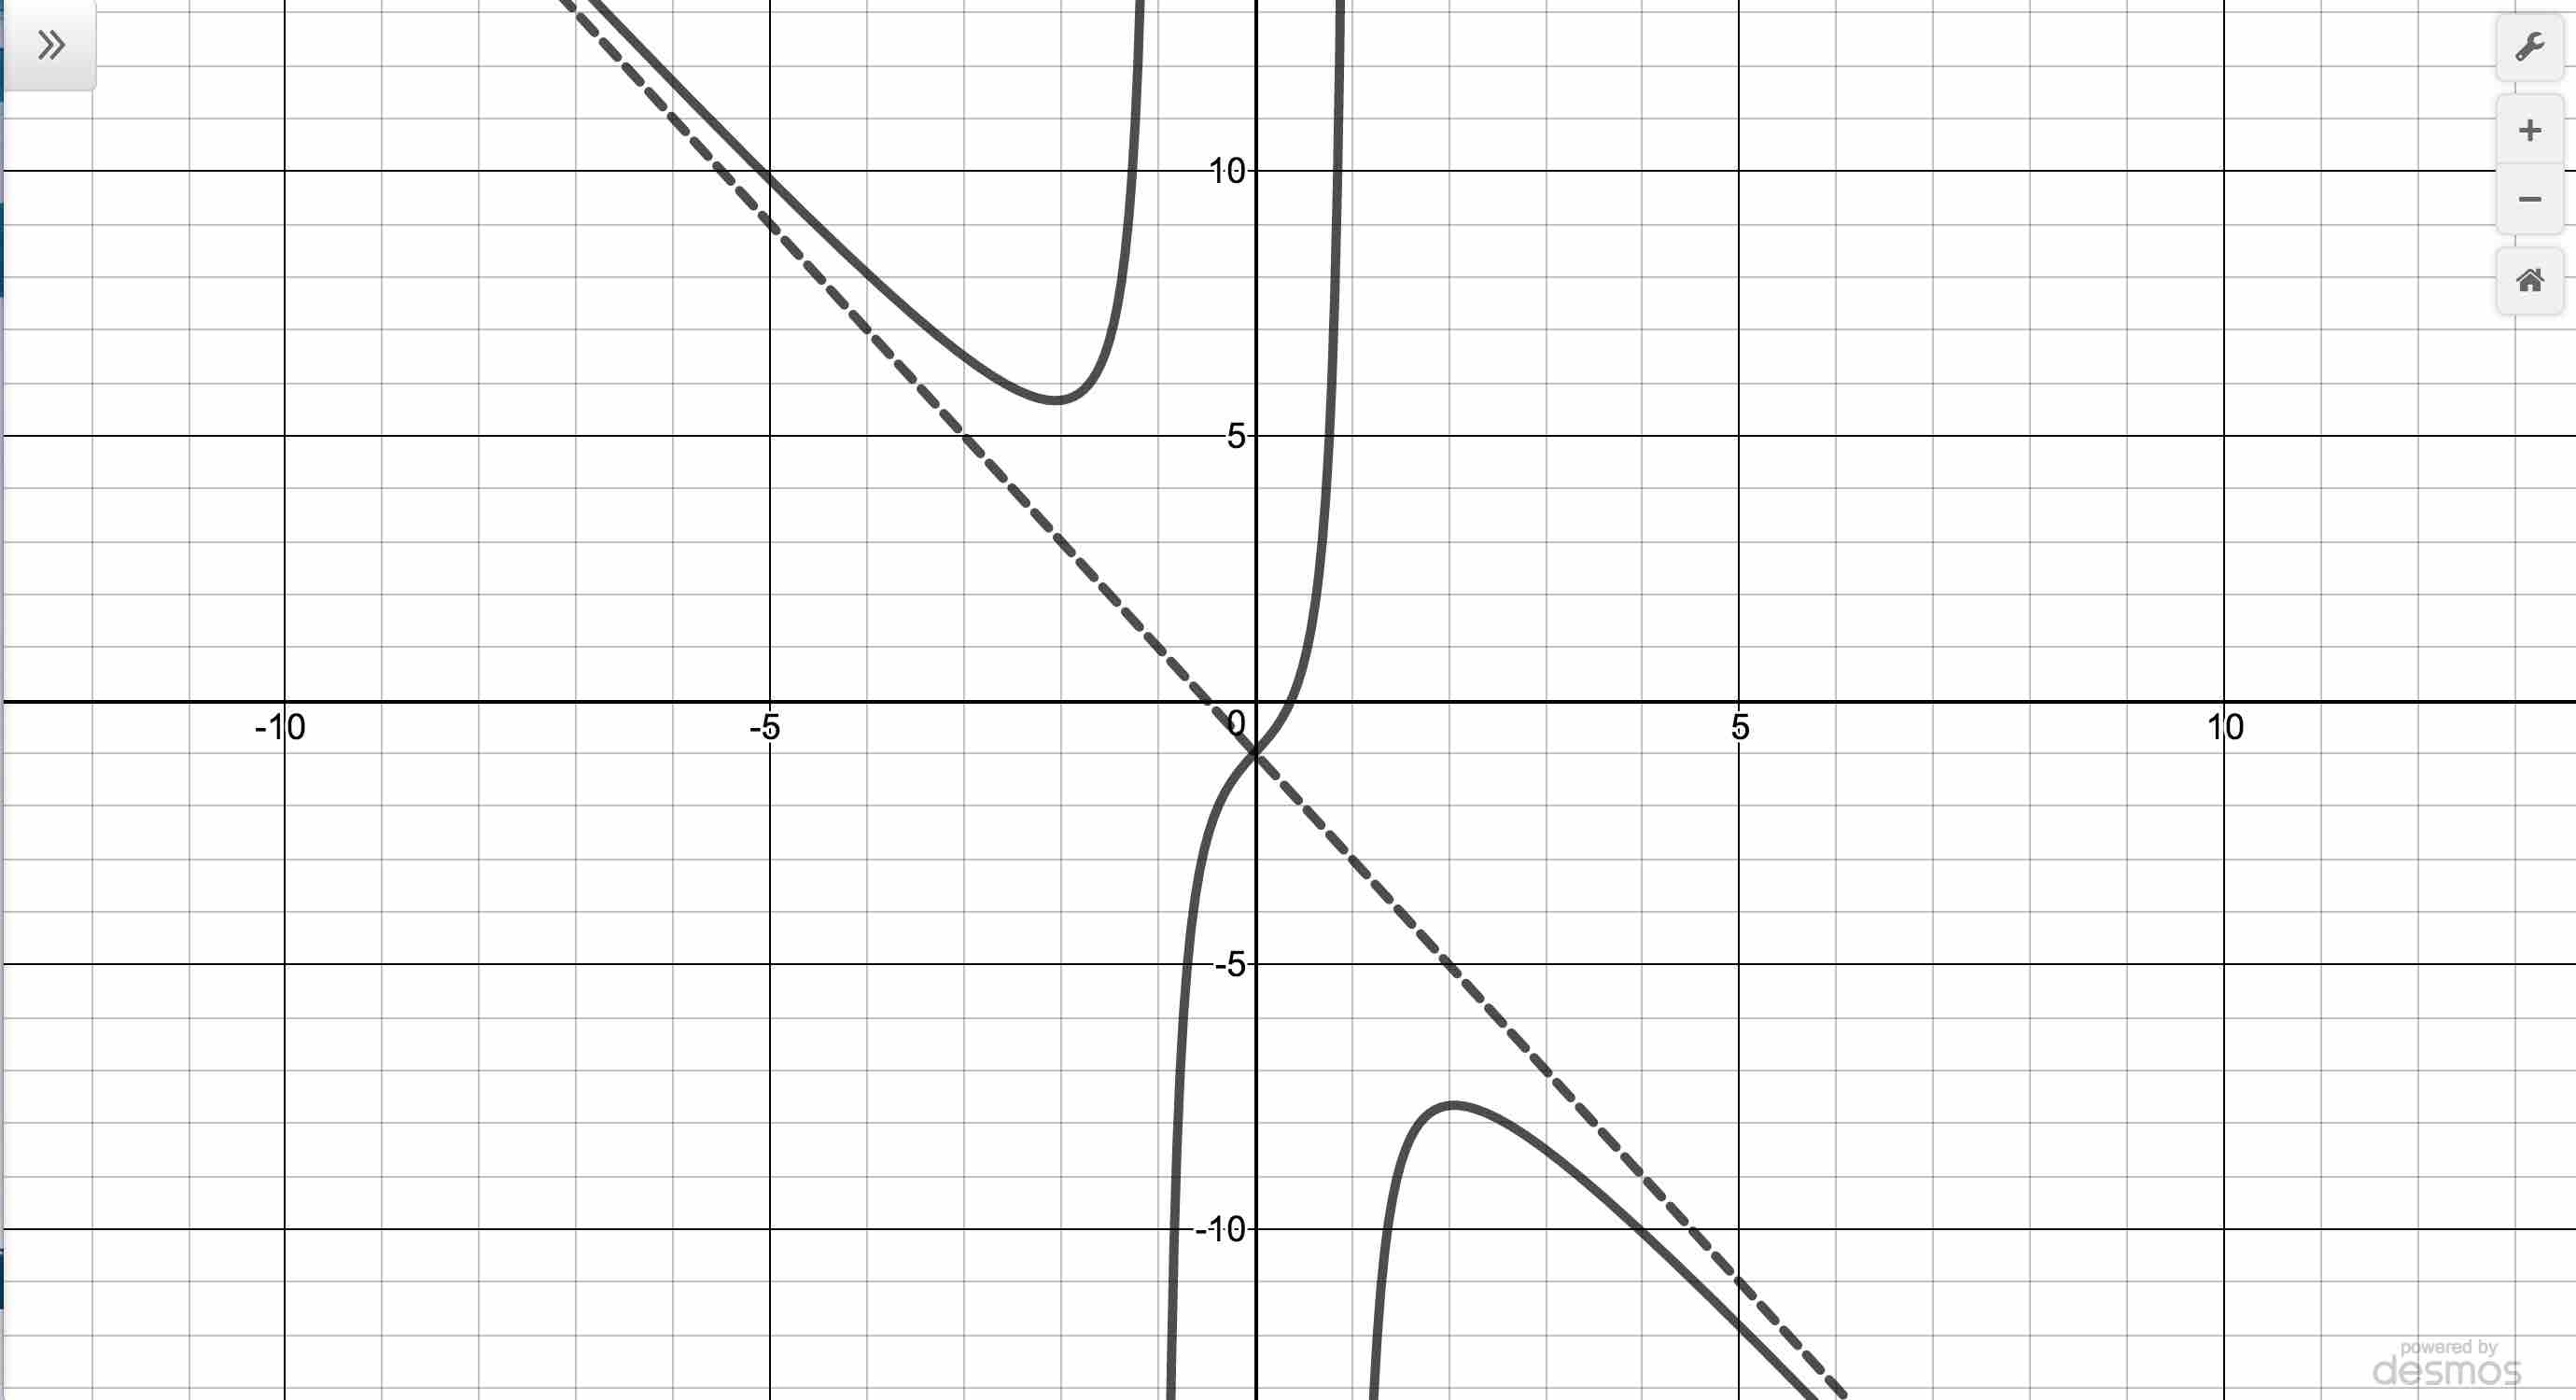
\includegraphics[width=3in]{./IntroRationalGraphics/SAEx05.jpg} \\
The graph of $y=h(x)$  & The graph of $y=r(t)$ \\


\end{tabular}
\end{center}

\qed

\end{enumerate}

\end{ex}

Our last example gives a real-world application of a slant asymptote. The problem features the concept of \textbf{average profit}. The average profit, denoted $\overline{P}(x)$,  is the total profit, $P(x)$,  divided by the number of items sold, $x$. In English, the average profit tells us the profit made per item sold. It, along with average cost, is defined below.

\colorbox{ResultColor}{\bbm

\begin{defn} \label{averagecostprofit} Let $C(x)$ and $P(x)$ represent the cost and profit to make and sell $x$ items, respectively.

\begin{itemize}

\item    The \index{average cost}\index{cost ! average} \textbf{average cost}, $\overline{C}(x) = \dfrac{C(x)}{x}$, $x > 0$.  

\textbf{NOTE:}  The average cost is the cost per item produced.

\item   The \index{average profit}\index{profit ! average} \textbf{average profit}, $\overline{P}(x) = \dfrac{P(x)}{x}$, $x > 0$.  

\textbf{NOTE:}  The average profit is the profit  per item sold.

\end{itemize}

\end{defn}

\ebm}

You'll explore average cost (and its relation to variable cost) in Exercise \ref{averagevariablecostexercise}.  For now, we refer the reader to to Example \ref{PortaBoyProfit}  in Section \ref{QuadraticFunctions}.

\begin{ex} \label{PortaBoyAverageProfit}  Recall the profit (in dollars) when $x$ PortaBoy game systems are produced and sold is given by $P(x) =  -1.5x^2+170x-150$, $0 \leq x \leq 166$.

\begin{enumerate}

\item  Find and simplify an expression for the average profit, $\overline{P}(x)$.  What is the domain of $\overline{P}$?

\item Find and interpret $\overline{P}(50)$.

\item Determine the slant asymptote to the graph of $y = \overline{P}(x)$.  Check your answer using a graphing utility.

\item  Interpret the slope of the slant asymptote.


\end{enumerate}

{\bf Solution.}

\begin{enumerate}

\item  We find $\overline{P}(x)  = \frac{P(x)}{x} = \frac{ -1.5x^2+170x-150}{x} = -1.5x + 170 + \frac{150}{x}$.  Since the domain of $P$ is $[0, 166]$ but $x \neq 0$, the domain of $\overline{P}$ is $(0, 166]$.

\item  We find $\overline{P}(50) = -1.5(50)+170 + \frac{150}{50} = 98$.  This means that when $50$ PortaBoy systems are sold, the average profit is $\$ 98$ per system.

\item  Technically, the graph of $y = \overline{P}(x)$ has no slant asymptote since the domain of the function is restricted to $(0, 166]$.  That being said, if we were to let $x \rightarrow \infty$, the term $\frac{150}{x} \rightarrow 0$, so we'd  have $\overline{P}(x)  \rightarrow -1.5x + 170$.  This means the slant asymptote would be $y = -1.5x + 170$.  We graph $y = \overline{P}(x)$ and $y = -1.5x+170$.

  
\begin{center}
   
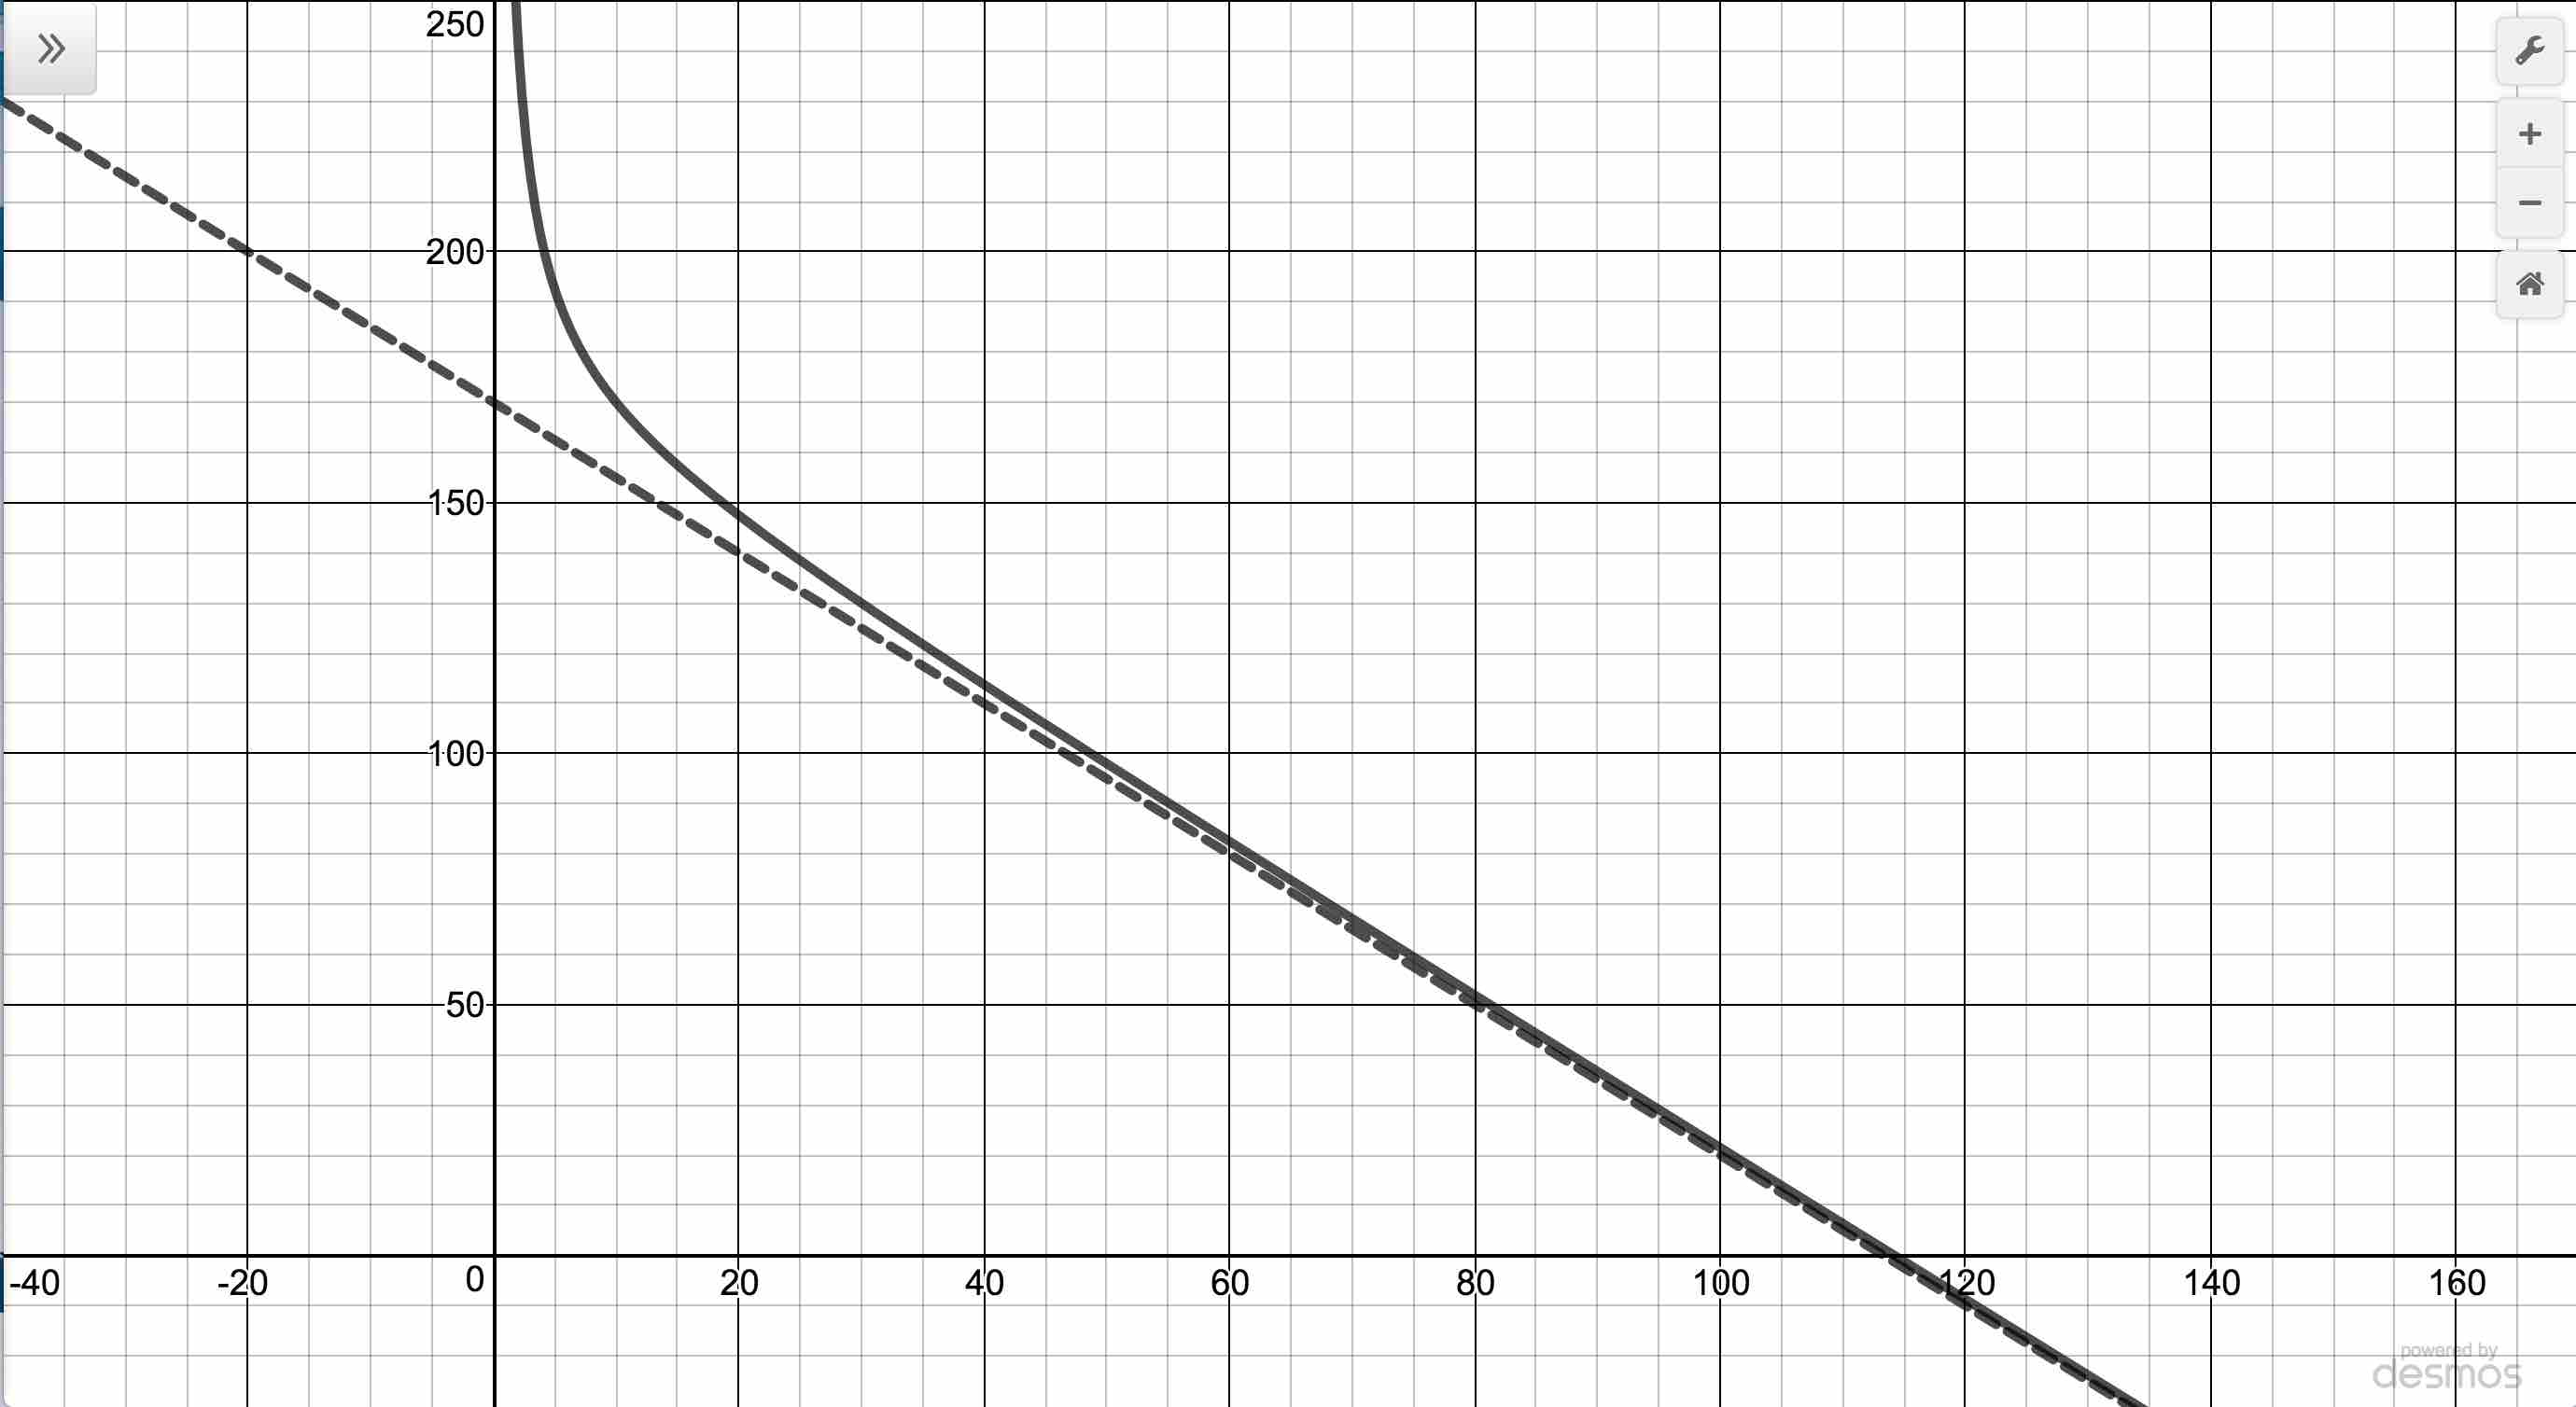
\includegraphics[width=4in]{./IntroRationalGraphics/SAEx06.jpg}

\end{center}

\item The slope of the slant asymptote $y = -1.5x+170$ is $-1.5$.  Allowing for $x \rightarrow \infty$, $\overline{P}(x) \approx -1.5 x + 170$ which means as we sell more systems, the average profit is \textbf{decreasing} at about a rate of $\$ 1.50$ per system.  If the number $1.5$ sounds familiar to this problem situation, it should.  In Example \ref{PortaBoyDemand} in Section \ref{ConstantandLinearFunctions}, we determined the slope of the demand function to be $-1.5$. In that situation, the $-1.5$ meant that in order to sell an additional system, the price had to drop by $\$ 1.50$.  The fact the average profit is decreasing at more or less this same rate means the loss in profit per system can be attributed to the reduction in price needed to sell each additional system.\footnote{We generalize this result in Exercise \ref{slantyintaverageprofitexercise}.} \qed

\end{enumerate}


\end{ex}

\newpage

\subsection{Exercises}

\documentclass{ximera}

\begin{document}
	\author{Stitz-Zeager}
	\xmtitle{TITLE}

\mfpicnumber{1}
\opengraphsfile{ExercisesforIntroRational}

(Review of Long Division):\footnote{For more review, see Section \ref{polylongdiv}.}  In Exercises \ref{longpolydivreviewfirst} - \ref{longpolydivreviewlast}, use polynomial long division to perform the indicated division.  Write the polynomial in the form $p(x) = d(x)q(x) + r(x)$.

\begin{multicols}{2}
\begin{enumerate}
\item $\left(4x^2+3x-1 \right) \div (x-3)$ \label{longpolydivreviewfirst}
\item $\left(2x^3-x+1 \right) \div \left(x^{2} +x+1 \right)$

\setcounter{HW}{\value{enumi}}
\end{enumerate}
\end{multicols}

\begin{multicols}{2}
\begin{enumerate}
\setcounter{enumi}{\value{HW}}

\item $\left(5x^{4} - 3x^{3} + 2x^{2} - 1 \right) \div \left(x^{2} + 4 \right)$
\item $\left(-x^{5} + 7x^{3} - x \right) \div \left(x^{3} - x^{2} + 1 \right)$

\setcounter{HW}{\value{enumi}}
\end{enumerate}
\end{multicols}

\begin{multicols}{2}
\begin{enumerate}
\setcounter{enumi}{\value{HW}}

\item $\left(9x^{3} + 5 \right) \div \left(2x - 3 \right)$
\item $\left(4x^2 - x - 23 \right) \div \left(x^{2} - 1 \right)$ \label{longpolydivreviewlast}

\setcounter{HW}{\value{enumi}}
\end{enumerate}
\end{multicols}


In Exercises \ref{rationaltransfirst} - \ref{rationaltranslast}, given the pair of functions $f$ and $F$, sketch the graph of $y=F(x)$ by starting with the graph of $y = f(x)$ and using Theorem \ref{linearlaurentlgraphs}.   Track at least two points and the asymptotes.  State the domain and range using interval notation.


\begin{multicols}{2}
\begin{enumerate}
\setcounter{enumi}{\value{HW}}
\item $f(x) = \dfrac{1}{x}$,  $F(x) = \dfrac{1}{x-2}+1$ \label{rationaltransfirst}
\item $f(x) =\dfrac{1}{x}$, $F(x) = \dfrac{2x}{x+1}$

\setcounter{HW}{\value{enumi}}
\end{enumerate}
\end{multicols}

\begin{multicols}{2}
\begin{enumerate}
\setcounter{enumi}{\value{HW}}

\item $f(x) =x^{-1}$, $F(x)=4x(2x+1)^{-1}$
\item $f(x) = x^{-2}$, $F(x)=-(x-1)^{-2}+3$  \label{rationaltranslast}

\setcounter{HW}{\value{enumi}}
\end{enumerate}
\end{multicols}


In Exercises \ref{findformulafor1overxgraphfirst} - \ref{findformulafor1overxgraphlast}, find a formula for each function below in the form $F(x) = \dfrac{a}{x-h}+k$.

\begin{multicols}{2}

\begin{enumerate}
\setcounter{enumi}{\value{HW}}

\item $~$ \label{findformulafor1overxgraphfirst}  $y=F(x)$ %$F(x) = \dfrac{1}{x+2}-1$

\begin{mfpic}[15]{-5}{5}{-5}{5}
\axes
\tlabel[cc](5,-0.5){\scriptsize $x$}
\tlabel[cc](0.5,5){\scriptsize $y$}
%\tlabel[cc](-1.5, 0.5){\scriptsize $(-1,0)$}
%\tlabel[cc](-0.5,-1){\scriptsize $\left(0, \frac{1}{2} \right)$}
\xmarks{-4,-3,-2,-1,1,2,3,4}
\ymarks{-4,-3,-2, -1, 1,2,3,4}
\tlpointsep{4pt}
\scriptsize
\axislabels {x}{ {$-4 \hspace{7pt}$} -4, {$-3 \hspace{7pt}$} -3, {$-2 \hspace{7pt}$} -2, {$-1 \hspace{7pt}$} -1, {$1$} 1, {$2$} 2, {$3$} 3, {$4$} 4}
\axislabels {y}{{$-1$} -1,{$1$} 1, {$2$} 2, {$3$} 3, {$4$} 4, {$-2$} -2, {$-3$} -3, {$-4$} -4}
\dashed \polyline{(-4.75,-1), (4.75,-1)}
\dashed \polyline{(-2,-4.75), (-2,4.75)}
\penwd{1.25pt}
\arrow \reverse \arrow \function{-5,-2.25,0.1}{1/(x+2)-1}
\arrow \reverse \arrow \function{-1.83,5,0.1}{1/(x+2)-1}
\point[4pt]{(-1,0), (0,-0.5)}
\tcaption{ \scriptsize $x$-intercept $(-1,0)$, $y$-intercept $\left(0, -\frac{1}{2}\right)$}
\normalsize
\end{mfpic}



\item $~$ \label{findformulafor1overxgraphlast} $y = F(x)$ %$F(x) = -\dfrac{2}{x-1}+1$

\begin{mfpic}[15]{-5}{5}{-5}{5}
\axes
\tlabel[cc](5,-0.5){\scriptsize $x$}
\tlabel[cc](0.5,5){\scriptsize $y$}
%\tlabel[cc](-1.5, 0.5){\scriptsize $(-1,0)$}
%\tlabel[cc](-0.5,-1){\scriptsize $\left(0, \frac{1}{2} \right)$}
\xmarks{-4,-3,-2,-1,1,2,3,4}
\ymarks{-4,-3,-2, -1, 1,2,3,4}
\tlpointsep{4pt}
\scriptsize
\axislabels {x}{ {$-4 \hspace{7pt}$} -4, {$-3 \hspace{7pt}$} -3, {$-2 \hspace{7pt}$} -2, {$-1 \hspace{7pt}$} -1, {$1$} 1, {$2$} 2, {$3$} 3, {$4$} 4}
\axislabels {y}{{$-1$} -1,{$1$} 1, {$2$} 2, {$3$} 3, {$4$} 4, {$-2$} -2, {$-3$} -3, {$-4$} -4}
\dashed \polyline{(-4.75,1), (4.75,1)}
\dashed \polyline{(1,-4.75), (1,4.75)}
\penwd{1.25pt}
\arrow \reverse \arrow \function{-5,0.45,0.1}{1-2/(x-1)}
\arrow \reverse \arrow \function{1.35,5,0.1}{1-2/(x-1)}
\point[4pt]{(3,0), (0,3)}
\tcaption{ \scriptsize $x$-intercept $(3,0)$, $y$-intercept $\left(0, 3 \right)$}
\normalsize
\end{mfpic}


\setcounter{HW}{\value{enumi}}

\end{enumerate}

\end{multicols}

\newpage

In Exercises \ref{findformulafor1overxsquaredgraphfirst} - \ref{findformula1overxsquaredgraphlast}, find a formula for each function below in the form $F(x) = \dfrac{a}{(x-h)^2}+k$.


\begin{multicols}{2}

\begin{enumerate}

\setcounter{enumi}{\value{HW}}

\item $~$ \label{findformulafor1overxsquaredgraphfirst} $y = F(x)$ %$F(x) = -\dfrac{4}{(x+2)^2}+4$

\begin{mfpic}[15]{-5}{5}{-5}{5}
\axes
\tlabel[cc](5,-0.5){\scriptsize $x$}
\tlabel[cc](0.5,5){\scriptsize $y$}
%\tlabel[cc](-1.5, 0.5){\scriptsize $(-1,0)$}
%\tlabel[cc](-0.5,-1){\scriptsize $\left(0, \frac{1}{2} \right)$}
\xmarks{-4,-3,-2,-1,1,2,3,4}
\ymarks{-4,-3,-2, -1, 1,2,3,4}
\tlpointsep{4pt}
\scriptsize
\axislabels {x}{ {$-4 \hspace{7pt}$} -4,{$-2 \hspace{7pt}$} -2,  {$1$} 1, {$2$} 2, {$3$} 3, {$4$} 4}
\axislabels {y}{{$-1$} -1,{$1$} 1, {$2$} 2, {$3$} 3, {$4$} 4, {$-2$} -2, {$-3$} -3, {$-4$} -4}
\dashed \polyline{(-4.75,4), (4.75,4)}
\dashed \polyline{(-2,-4.75), (-2,4.75)}
\penwd{1.25pt}
\arrow \reverse \arrow \function{-5,-2.7,0.1}{4-4/((x+2)**2)}
\arrow \reverse \arrow \function{-1.3,5,0.1}{4-4/((x+2)**2)}
\point[4pt]{(-3,0), (-1,0), (0,3)}
\tcaption{\scriptsize $x$-intercepts $(-3,0)$,  $(-1,0)$, $y$-intercept $(0,3)$}
\normalsize
\end{mfpic}


\item $~$  \label{findformula1overxsquaredgraphlast}$y = F(x)$ %$F(x) = \dfrac{4}{(2x-1)^2}-4$

\begin{mfpic}[15]{-5}{5}{-5}{5}
\axes
\tlabel[cc](5,-0.5){\scriptsize $x$}
\tlabel[cc](0.5,5){\scriptsize $y$}
%\tlabel[cc](-1.5, 0.5){\scriptsize $(-1,0)$}
%\tlabel[cc](-0.5,-1){\scriptsize $\left(0, \frac{1}{2} \right)$}
\xmarks{-4,-3,-2,-1,1,2,3,4}
\ymarks{-4,-3,-2, -1, 1,2,3,4}
\tlpointsep{4pt}
\scriptsize
\axislabels {x}{ {$-4 \hspace{7pt}$} -4, {$-3 \hspace{7pt}$} -3, {$-2 \hspace{7pt}$} -2, {$-1 \hspace{7pt}$} -1, {$1$} 1, {$2$} 2, {$3$} 3, {$4$} 4}
\axislabels {y}{{$-1$} -1,{$1$} 1, {$2$} 2, {$3$} 3, {$4$} 4, {$-2$} -2, {$-4$} -4}
\dashed \polyline{(-4.75,-4), (4.75,-4)}
\dashed \polyline{(0.5,-4.75), (0.5,4.75)}
\penwd{1.25pt}
\arrow \reverse \arrow \function{-5, 0.16, 0.1}{4/((2*x-1)**2) - 4}
\arrow \reverse \arrow \function{0.84, 5, 0.1}{4/((2*x-1)**2) - 4}
\point[4pt]{(0,0), (1,0)}
\tcaption{\scriptsize $x$-intercepts $(0,0)$,  $(1,0)$, Vertical Asymptote:  $x = \frac{1}{2}$}
\normalsize
\end{mfpic}



\setcounter{HW}{\value{enumi}}

\end{enumerate}

\end{multicols}



In Exercises \ref{alltheasympfirst} - \ref{alltheasymplast}, for the given rational function:

\begin{multicols}{2}
\begin{itemize}

\item State the domain.
\item Identify any vertical asymptotes of the graph.

\end{itemize}
\end{multicols}

\begin{multicols}{2}
\begin{itemize}

\item Identify any holes in the graph.
\item Find the horizontal asymptote, if it exists.

\end{itemize}
\end{multicols}

\begin{multicols}{2}
\begin{itemize}

\item Find the slant asymptote, if it exists.
\item Graph the function using a graphing utility and describe the behavior near the asymptotes.

\end{itemize}
\end{multicols}

\begin{multicols}{3}
\begin{enumerate}
\setcounter{enumi}{\value{HW}}

\item $f(x) = \dfrac{x}{3x - 6}$ \label{alltheasympfirst}
\item $f(x) = \dfrac{3 + 7x}{5 - 2x}$
\item $f(x) = \dfrac{x}{x^{2} + x - 12}$

\setcounter{HW}{\value{enumi}}
\end{enumerate}
\end{multicols}

\begin{multicols}{3}
\begin{enumerate}
\setcounter{enumi}{\value{HW}}

\item $g(t) = \dfrac{t}{t^{2} + 1}$
\item $g(t) = \dfrac{t + 7}{(t + 3)^{2}}$
\item $g(t) = \dfrac{t^{3} + 1}{t^{2} - 1}$

\setcounter{HW}{\value{enumi}}
\end{enumerate}
\end{multicols}

\begin{multicols}{3}
\begin{enumerate}
\setcounter{enumi}{\value{HW}}

\item $r(z) = \dfrac{4z}{z^2+4}$
\item $r(z) = \dfrac{4z}{z^2-4}$
\item $r(z) = \dfrac{z^2-z-12}{z^2+z-6}$

\setcounter{HW}{\value{enumi}}
\end{enumerate}
\end{multicols}

\begin{multicols}{3}
\begin{enumerate}
\setcounter{enumi}{\value{HW}}

\item $f(x) = \dfrac{3x^2-5x-2}{x^2-9}$
\item $f(x) = \dfrac{x^3+2x^2+x}{x^2-x-2}$
\item $f(x) = \dfrac{x^{3} - 3x + 1}{x^{2} + 1}$

\setcounter{HW}{\value{enumi}}
\end{enumerate}
\end{multicols}

\begin{multicols}{3}
\begin{enumerate}
\setcounter{enumi}{\value{HW}}

\item $g(t) = \dfrac{2t^{2} + 5t - 3}{3t + 2}$
\item $g(t) = \dfrac{-t^{3} + 4t}{t^{2} - 9}$
\item \small $g(t) = \dfrac{-5t^{4} - 3t^{3} + t^{2} - 10}{t^{3} - 3t^{2} + 3t - 1}$ \normalsize

\setcounter{HW}{\value{enumi}}
\end{enumerate}
\end{multicols}


\begin{multicols}{3}
\begin{enumerate}
\setcounter{enumi}{\value{HW}}

\item $r(z) = \dfrac{z^3}{1-z}$
\item $r(z) = \dfrac{18-2z^2}{z^2-9}$
\item $r(z) = \dfrac{z^3-4z^2-4z-5}{z^2+z+1}$ \label{alltheasymplast}


\setcounter{HW}{\value{enumi}}
\end{enumerate}
\end{multicols}

\newpage

\begin{enumerate}
\setcounter{enumi}{\value{HW}}



\item The cost $C(p)$ in dollars to remove $p$\% of the invasive  Ippizuti fish species from Sasquatch Pond is: \[C(p) = \frac{1770p}{100 - p}, \quad 0 \leq p < 100 \]

\begin{enumerate}

\item Find and interpret $C(25)$ and $C(95)$.
\item What does the vertical asymptote at $x = 100$ mean within the context of the problem?
\item What percentage of the Ippizuti fish can you remove for  \$40000?

\end{enumerate}

\item  In the scenario of  Example \ref{averagevelocityrocketex}, $s(t) = -5t^2+100t$, $0 \leq t \leq 20$ gives the height of a model rocket above the Moon's surface, in feet,  $t$ seconds after liftoff.  For each of the times $t_{0}$ listed below, find and simplify a the formula for the average velocity $\overline{v}(t)$ between $t$ and $t_{0}$ (see Definition \ref{averagevelocitydefn}) and use $\overline{v}(t)$ to find and interpret the instantaneous velocity of the rocket at $t = t_{0}$ (See Example \ref{averagevelocityrocketex}).

\begin{multicols}{4}

\begin{enumerate}

\item  $t_{0} = 5$

\item $t_{0} = 9$

\item $t_{0} = 10$

\item  $t_{0} = 11$

\end{enumerate}

\end{multicols}


\item \label{squatchpop} The population of Sasquatch in Portage County $t$ years after the year 1803 is modeled by the function \[P(t) = \frac{150t}{t + 15}.\] Find and interpret the horizontal asymptote of the graph of $y = P(t)$ and explain what it means.

\item  The cost in dollars, $C(x)$ to make $x$ dOpi media players is $C(x) = 100x+2000$, $x \geq 0$.  You may wish to review the concepts of fixed and variable costs introduced in  Example \ref{PortaBoyCost} in Section \ref{LinearFunctions}.

\begin{enumerate}

\item  Find a formula for the average cost $\overline{C}(x)$.

\item  Find and interpret $\overline{C}(1)$ and $\overline{C}(100)$.

\item  How many dOpis need to be produced so that the average cost per dOpi is $\$ 200$?

\item  Find and interpret $\ds{ \lim_{x \rightarrow 0^{+}} \overline{C}(x)}$.

\item  Interpret the behavior of $\overline{C}(x)$ as $x \rightarrow \infty$.

\end{enumerate}

\item  \label{averagevariablecostexercise}   This exercise explores the relationships between fixed cost, variable cost, and average cost.  The reader is encouraged to revisit Example \ref{PortaBoyCost} in Section \ref{LinearFunctions} as needed.  Suppose the cost in dollars $C(x)$ to make $x$ items is given by $C(x) = mx + b$ where $m$ and $b$ are positive real numbers.

\begin{enumerate}

\item  Show the fixed cost (the money spent even if no items are made) is $b$.
\item  Show the variable cost (the increase in cost per item made) is $m$.
\item  Find a formula for the average cost when making $x$ items, $\overline{C}(x)$.
\item  Show $\overline{C}(x) > m$ for all $x>0$ and, moreover,   $\overline{C}(x)  \rightarrow m^{+}$ as $x \rightarrow \infty$.
\item  Interpret $\overline{C}(x)  \rightarrow m^{+}$ both geometrically and in terms of fixed, variable, and average costs.

\end{enumerate}

\item  \label{slantyintaverageprofitexercise} Suppose the price-demand function for a particular product is given by $p(x) = mx + b$  where $x$ is the number of items made and sold for $p(x)$ dollars.  Here,  $m<0$ and $b>0$.  If the cost (in dollars) to make $x$ of these products is also a linear  function $C(x)$, show that the graph of the average profit function $\overline{P}(x)$ has a slant asymptote with slope $m$ and interpret.

\item In Exercise \ref{circuitexercisepoly} in Section \ref{GraphsofPolynomials}, we fit a few polynomial models to the following electric circuit data. The circuit was built with a variable resistor.  For each of the following resistance values (measured in kilo-ohms, $k \Omega$),  the corresponding power to the load (measured in milliwatts, $mW$) is given below.\footnote{The authors wish to thank Don Anthan and Ken White of Lakeland Community College for devising this problem and generating the accompanying data set.}


\smallskip

\noindent \begin{tabular}{|l|r|r|r|r|r|r|} \hline
Resistance: ($k \Omega$) & 1.012 & 2.199 & 3.275 & 4.676 & 6.805 & 9.975 \\ \hline
Power: ($mW$) & 1.063 & 1.496 & 1.610 & 1.613 & 1.505 & 1.314 \\ \hline
\end{tabular}

\smallskip

\noindent Using some fundamental laws of circuit analysis mixed with a healthy dose of algebra, we can derive the actual formula relating power $P(x)$ to resistance $x$:   \[P(x) = \frac{25x}{(x + 3.9)^2}, \quad x \geq 0.\]

\begin{enumerate}

\item Graph the data along with the function $y = P(x)$ using a graphing utility.

\item Use a graphing utility to approximate the maximum power that can be delivered to the load.  What is the corresponding resistance value?

\item Find and interpret the end behavior of $P(x)$ as $x \rightarrow \infty$.

\end{enumerate}


\item  Let $f(x) = \dfrac{ax^2-c}{x+3}$.  Find values  for $a$ and  $c$ so  the graph of $f$ has a hole  at $(-3, 12)$.

\item  Let  $f(x) = \dfrac{ax^{n} -4}{2x^2+1}$.

\begin{enumerate}

\item  Find values for $a$ and $n$ so the graph of $y = f(x)$  has the horizontal asymptote $y = 3$.

\item  Find values for $a$ and $n$ so the graph of  $y=f(x)$ has the slant asymptote $y = 5x$.

\end{enumerate}


\item  Suppose $p$ is a polynomial function and $a$ is a real number.  Define $r(x)= \dfrac{p(x) - p(a)}{x-a}$.  Use the Factor Theorem, Theorem \ref{factorthm}, to prove the graph of $y = r(x)$ has a hole at $x =a$.


\item \label{laurentarcexercise}For each function $f(x)$ listed below, compute the average rate of change over the indicated interval.\footnote{See Definition \ref{arc} in Section \ref{AverageRateofChange} for a review of this concept, as needed.}  What trends do you observe?  How do your answers manifest themselves graphically?  How do you results compare with those of Exercise \ref{monomialarcexercise} in Section \ref{GraphsofPolynomials}?

\vspace*{-0.2in}

\[ \begin{array}{|r||c|c|c|c|}  \hline

 f(x) &  [0.9, 1.1] & [0.99, 1.01] &[0.999, 1.001] & [0.9999, 1.0001]  \\ \hline
 x^{-1} &&&&   \\  \hline
 x^{-2} &&&&    \\  \hline
 x^{-3} &&&&   \\  \hline
 x^{-4} &&&&   \\  \hline
\end{array} \]

\item \index{Learning Curve Equation} \index{Thurstone, Louis Leon} In his now famous 1919 dissertation \underline{The Learning Curve Equation}, Louis Leon Thurstone presents a rational function which models the number of words a person can type in four minutes as a function of the number of pages of practice one has completed.\footnote{This paper, which is now in the public domain and can be found  \href{http://bit.ly/2uNaUBa}{\underline{here}}, is from a bygone era when students at business schools took typing classes on manual typewriters.} Using his original notation and original language, we have $Y = \frac{L(X + P)}{(X + P) + R}$ where $L$ is the predicted practice limit in terms of speed units, $X$ is pages written, $Y$ is writing speed in terms of words in four minutes, $P$ is equivalent previous practice in terms of pages and $R$ is the rate of learning. In Figure 5 of the paper, he graphs a scatter plot and the curve $Y = \frac{216(X + 19)}{X + 148}$.  Discuss this equation with your classmates.  How would you update the notation?  Explain what the horizontal asymptote of the graph means.  You should take some time to look at the original paper. Skip over the computations you don't understand yet and try to get a sense of the time and place in which the study was conducted.

\end{enumerate}

\newpage

\subsection{Answers}

\begin{enumerate}
\item $4x^2+3x-1 = (x-3)(4x+15) + 44$
\item $2x^3-x+1 = \left(x^2+x+1\right)(2x-2)+(-x+3)$
\item $5x^{4} - 3x^{3} + 2x^{2} - 1 = \left(x^{2} + 4 \right) \left(5x^{2} - 3x - 18 \right) + (12x + 71)$
\item $-x^{5} + 7x^{3} - x = \left(x^{3} - x^{2} + 1 \right) \left(-x^{2} - x + 6 \right) + \left(7x^{2} - 6 \right)$
\item $9x^{3} + 5 =(2x - 3) \left(\frac{9}{2}x^{2} + \frac{27}{4}x + \frac{81}{8} \right) + \frac{283}{8}$
\item $4x^2 - x - 23 = \left(x^{2} - 1 \right)(4) + (-x - 19)$
\setcounter{HW}{\value{enumi}}
\end{enumerate}


\begin{multicols}{2}
\begin{enumerate}
\setcounter{enumi}{\value{HW}}

\item $F(x) = \dfrac{1}{x-2}+1$ \\ [10pt]
Domain: $(-\infty, 2) \cup (2, \infty)$ \\
Range: $(-\infty, 1) \cup (1, \infty)$ \\
Vertical asymptote:  $x = 2$\\
Horizontal asymptote:  $y = 1$ \\

\begin{mfpic}[15]{-5}{5}{-5}{5}
\axes
\tlabel[cc](5,-0.5){\scriptsize $x$}
\tlabel[cc](0.5,5){\scriptsize $y$}
%\tlabel[cc](-1.5, 0.5){\scriptsize $(-1,0)$}
%\tlabel[cc](-0.5,-1){\scriptsize $\left(0, \frac{1}{2} \right)$}
\xmarks{-4,-3,-2,-1,1,2,3,4}
\ymarks{-4,-3,-2, -1, 1,2,3,4}
\tlpointsep{4pt}
\scriptsize
\axislabels {x}{ {$-4 \hspace{7pt}$} -4, {$-3 \hspace{7pt}$} -3, {$-2 \hspace{7pt}$} -2, {$-1 \hspace{7pt}$} -1, {$1$} 1, {$2$} 2, {$3$} 3, {$4$} 4}
\axislabels {y}{{$-1$} -1,{$1$} 1, {$2$} 2, {$3$} 3, {$4$} 4, {$-2$} -2, {$-3$} -3, {$-4$} -4}
\dashed \polyline{(-4.75,1), (4.75,1)}
\dashed \polyline{(2,-4.75), (2,4.75)}
\penwd{1.25pt}
\arrow \reverse \arrow \function{-5,1.8,0.1}{1+1/(x-2)}
\arrow \reverse \arrow \function{2.3,5,0.1}{1+1/(x-2)}
\point[4pt]{(1,0), (3,2)}
\normalsize
\end{mfpic}


\vfill

\columnbreak

\item $F(x) = \dfrac{2x}{x+1} = \dfrac{-2}{x+1}+2$\\ [10pt]
Domain: $(-\infty, -1) \cup (-1, \infty)$ \\
Range: $(-\infty, 2) \cup (2, \infty)$ \\
Vertical asymptote:  $x = -1$\\
Horizontal asymptote:  $y = 2$ \\

\begin{mfpic}[15]{-5}{5}{-5}{5}
\axes
\tlabel[cc](5,-0.5){\scriptsize $x$}
\tlabel[cc](0.5,5){\scriptsize $y$}
%\tlabel[cc](-1.5, 0.5){\scriptsize $(-1,0)$}
%\tlabel[cc](-0.5,-1){\scriptsize $\left(0, \frac{1}{2} \right)$}
\xmarks{-4,-3,-2,-1,1,2,3,4}
\ymarks{-4,-3,-2, -1, 1,2,3,4}
\tlpointsep{4pt}
\scriptsize
\axislabels {x}{ {$-4 \hspace{7pt}$} -4, {$-3 \hspace{7pt}$} -3, {$-2 \hspace{7pt}$} -2, {$-1 \hspace{7pt}$} -1, {$1$} 1, {$2$} 2, {$3$} 3, {$4$} 4}
\axislabels {y}{{$1$} 1, {$2$} 2, {$3$} 3, {$4$} 4}
\dashed \polyline{(-4.75,2), (4.75,2)}
\dashed \polyline{(-1,-4.75), (-1,4.75)}
\penwd{1.25pt}
\arrow \reverse \arrow \function{-5,-1.7,0.1}{2x/(x+1)}
\arrow \reverse \arrow \function{-0.7,5,0.1}{2x/(x+1)}
\point[4pt]{(0,0), (-2,4)}
\normalsize
\end{mfpic}

\setcounter{HW}{\value{enumi}}
\end{enumerate}
\end{multicols}



\begin{multicols}{2}
\begin{enumerate}
\setcounter{enumi}{\value{HW}}

\item $F(x)=4x(2x+1)^{-1} = \dfrac{4x}{2x+1} = \dfrac{-1}{x+\frac{1}{2}}+2$ \\ [10pt]
Domain: $\left(-\infty, -\frac{1}{2} \right) \cup \left(-\frac{1}{2},  \infty \right)$ \\
Range: $(-\infty, 2) \cup (2, \infty)$ \\
Vertical asymptote:  $x  = -\frac{1}{2}$ \\
Horizontal asymptote: $y= 2$\\ 

\begin{mfpic}[15]{-5}{5}{-5}{5}
\axes
\tlabel[cc](5,-0.5){\scriptsize $x$}
\tlabel[cc](0.5,5){\scriptsize $y$}
%\tlabel[cc](-1.5, 0.5){\scriptsize $(-1,0)$}
%\tlabel[cc](-0.5,-1){\scriptsize $\left(0, \frac{1}{2} \right)$}
\xmarks{-4,-3,-2,-1,1,2,3,4}
\ymarks{-4,-3,-2, -1, 1,2,3,4}
\tlpointsep{4pt}
\scriptsize
\axislabels {x}{ {$-4 \hspace{7pt}$} -4, {$-3 \hspace{7pt}$} -3, {$-2 \hspace{7pt}$} -2, {$-1 \hspace{7pt}$} -1, {$1$} 1, {$2$} 2, {$3$} 3, {$4$} 4}
\axislabels {y}{{$1$} 1, {$2$} 2, {$3$} 3, {$4$} 4}
\dashed \polyline{(-4.75,2), (4.75,2)}
\dashed \polyline{(-0.5,-4.75), (-0.5,4.75)}
\penwd{1.25pt}
\arrow \reverse \arrow \function{-5,-0.84,0.1}{4*x/(2*x+1)}
\arrow \reverse \arrow \function{-0.35,5,0.1}{4*x/(2*x+1)}
\point[4pt]{(-1.5,3), (0.5,1)}
\normalsize
\end{mfpic}


\vfill

\columnbreak

\item $F(x)=-(x-1)^{-2}+3 = \dfrac{-1}{(x-1)^2} + 3$\\[10pt]
Domain: $(-\infty, 1) \cup (1, \infty)$ \\
Range: $(-\infty, 3) \cup (3, \infty)$ \\
Vertical asymptote:  $x = 1$\\
Horizontal asymptote:  $y = 3$ \\

\begin{mfpic}[15]{-5}{5}{-5}{5}
\axes
\tlabel[cc](5,-0.5){\scriptsize $x$}
\tlabel[cc](0.5,5){\scriptsize $y$}
%\tlabel[cc](-1.5, 0.5){\scriptsize $(-1,0)$}
%\tlabel[cc](-0.5,-1){\scriptsize $\left(0, \frac{1}{2} \right)$}
\xmarks{-4,-3,-2,-1,1,2,3,4}
\ymarks{-4,-3,-2, -1, 1,2,3,4}
\tlpointsep{4pt}
\scriptsize
\axislabels {x}{ {$-4 \hspace{7pt}$} -4, {$-3 \hspace{7pt}$} -3, {$-2 \hspace{7pt}$} -2, {$-1 \hspace{7pt}$} -1,  {$2$} 2, {$3$} 3, {$4$} 4}
\axislabels {y}{{$1$} 1, {$2$} 2, {$3$} 3, {$4$} 4, {$-1$} -1, {$-2$} -2, {$-3$} -3, {$-4$} -4}
\dashed \polyline{(-4.75,3), (4.75,3)}
\dashed \polyline{(1,-4.75), (1,4.75)}
\penwd{1.25pt}
\arrow \reverse \arrow \function{-5,0.64,0.1}{3-1/((x-1)**2)}
\arrow \reverse \arrow \function{1.36,5,0.1}{3-1/((x-1)**2)}
\point[4pt]{(0,2), (2,2)}
\normalsize
\end{mfpic}

\setcounter{HW}{\value{enumi}}
\end{enumerate}
\end{multicols}

\begin{multicols}{2}
\begin{enumerate}
\setcounter{enumi}{\value{HW}}

\item $F(x) = \dfrac{1}{x+2}-1$

\item  $F(x) = \dfrac{-2}{x-1}+1$

\setcounter{HW}{\value{enumi}}
\end{enumerate}
\end{multicols}


\begin{multicols}{2}

\begin{enumerate}

\setcounter{enumi}{\value{HW}}

\item  $F(x) = \dfrac{-4}{(x+2)^2}+4$  \vphantom{$F(x) = \dfrac{1}{\left(x-\frac{1}{2}\right)^2}-4$}

\item $F(x) = \dfrac{1}{\left(x-\frac{1}{2}\right)^2}-4$

\setcounter{HW}{\value{enumi}}
\end{enumerate}
\end{multicols}



\begin{multicols}{2}
\begin{enumerate}
\setcounter{enumi}{\value{HW}}

\item $f(x) = \dfrac{x}{3x - 6}$ \vphantom{$\dfrac{7x}{7x}$}\\
Domain: $(-\infty, 2) \cup (2, \infty)$\\
Vertical asymptote: $x = 2$\\
$\ds{\lim_{x \rightarrow 2^{-}} f(x) = -\infty}$, $\ds{\lim_{x \rightarrow 2^{+}} f(x) = \infty}$ \\
No holes in the graph\\
Horizontal asymptote: $y = \frac{1}{3}$ \\
$\ds{\lim_{x \rightarrow  -\infty} f(x) =}$ $\frac{1}{3}$\\
More specifically: as $x \rightarrow -\infty, f(x) \rightarrow \frac{1}{3}^{-}$\\
$\ds{\lim_{x \rightarrow  \infty} f(x) =}$ $\frac{1}{3}$\\
More specifically:  as $x \rightarrow \infty, f(x) \rightarrow \frac{1}{3}^{+}$\\

\vfill

\columnbreak

\item $f(x) = \dfrac{3 + 7x}{5 - 2x}$\\
Domain: $(-\infty, \frac{5}{2}) \cup (\frac{5}{2}, \infty)$\\
Vertical asymptote: $x = \frac{5}{2}$\\
$\ds{\lim_{x \rightarrow \frac{5}{2}^{-}} f(x) = \infty}$, $\ds{\lim_{x \rightarrow \frac{5}{2}^{+}} f(x) = -\infty}$ \\
No holes in the graph\\
Horizontal asymptote: $y = -\frac{7}{2}$ \\
$\ds{\lim_{x \rightarrow - \infty} f(x) =}$ $-\frac{7}{2}$\\
More specifically: as $x \rightarrow -\infty, f(x) \rightarrow -\frac{7}{2}^{+}$\\
$\ds{\lim_{x \rightarrow  \infty} f(x) =}$ $-\frac{7}{2}$\\
More specifically: as  $x \rightarrow \infty, f(x) \rightarrow -\frac{7}{2}^{-}$\\

\setcounter{HW}{\value{enumi}}
\end{enumerate}
\end{multicols}

\pagebreak 

\begin{multicols}{2}
\begin{enumerate}
\setcounter{enumi}{\value{HW}}

\item $f(x) = \dfrac{x}{x^{2} + x - 12} = \dfrac{x}{(x + 4)(x - 3)}$\\
Domain: $(-\infty, -4) \cup (-4, 3) \cup (3, \infty)$\\
Vertical asymptotes: $x = -4, x = 3$\\
$\ds{\lim_{x \rightarrow -4^{-}} f(x) =  -\infty}$ , $\ds{\lim_{x \rightarrow -4^{+}} f(x) =  \infty}$ \\
$\ds{\lim_{x \rightarrow 3^{-}} f(x) =  -\infty}$ , $\ds{\lim_{x \rightarrow 3^{+}} f(x) =  \infty}$ \\
No holes in the graph\\
Horizontal asymptote: $y = 0$ \\
$\ds{\lim_{x \rightarrow - \infty} f(x) = 0}$\\
More specifically, as  $x \rightarrow -\infty, f(x) \rightarrow 0^{-}$\\
$\ds{\lim_{x \rightarrow  \infty} f(x) = 0}$\\
More specifically, as $x \rightarrow \infty, f(x) \rightarrow 0^{+}$\\



\columnbreak


\item $g(t) = \dfrac{t}{t^{2} + 1}$\\
Domain: $(-\infty, \infty)$\\
No vertical asymptotes\\
No holes in the graph\\
Horizontal asymptote: $y = 0$ \\
$\ds{\lim_{t \rightarrow  - \infty} g(t) = 0}$\\
More specifically, as $t \rightarrow -\infty, g(t) \rightarrow 0^{-}$\\
$\ds{\lim_{t \rightarrow   \infty} g(t) = 0}$\\
More specifically, as $t \rightarrow \infty, g(t) \rightarrow 0^{+}$\\

\setcounter{HW}{\value{enumi}}
\end{enumerate}
\end{multicols}

\begin{multicols}{2}
\begin{enumerate}
\setcounter{enumi}{\value{HW}}

\item $g(t) = \dfrac{t + 7}{(t + 3)^{2}}$ \vphantom{$\dfrac{t^{3}}{t^{2}}$}\\
Domain: $(-\infty, -3) \cup (-3, \infty)$\\
Vertical asymptote: $t = -3$\\
$\ds{\lim_{t \rightarrow -3} g(t) =  \infty}$ \\
No holes in the graph\\
Horizontal asymptote: $y = 0$ \\
$\ds{\lim_{t \rightarrow - \infty} g(t) = 0}$\\
\footnote{This is hard to see on the calculator, but trust me, the graph is below the $t$-axis to the left of $t = -7$.}More specifically, as $t \rightarrow -\infty, g(t) \rightarrow 0^{-}$\\
$\ds{\lim_{t \rightarrow \infty} g(t) = 0}$\\
More specifically, as $t \rightarrow \infty, g(t) \rightarrow 0^{+}$\\

\vfill

\columnbreak

\item $g(t) = \dfrac{t^{3} + 1}{t^{2} - 1} = \dfrac{t^{2} - t+ 1}{t-1}$\\
Domain: $(-\infty, -1) \cup (-1, 1) \cup (1, \infty)$\\
Vertical asymptote: $t = 1$\\
$\ds{\lim_{t \rightarrow 1^{-}} g(t) =  -\infty}$, $\ds{\lim_{t \rightarrow 1^{+}} g(t) =  \infty}$ \\
Hole at $(-1, -\frac{3}{2})$\\
Slant asymptote: $y=t$  \\
$\ds{\lim_{t \rightarrow -\infty} g(t) = -\infty}$\\
As $t \rightarrow -\infty$, the graph is below $y=t$\\
$\ds{\lim_{t \rightarrow \infty} g(t) = \infty}$\\
As $t \rightarrow \infty$, the graph is above $y=t$\\

\setcounter{HW}{\value{enumi}}
\end{enumerate}
\end{multicols}

\begin{multicols}{2}
\begin{enumerate}
\setcounter{enumi}{\value{HW}}

\item $r(z) = \dfrac{4z}{z^{2} + 4}$\\
Domain: $(-\infty,  \infty)$\\
No vertical asymptotes \\
No holes in the graph\\
Horizontal asymptote: $y = 0$ \\
$\ds{\lim_{z \rightarrow - \infty} r(z) =0}$\\
More specifically, as $z \rightarrow -\infty, r(z) \rightarrow 0^{-}$\\
$\ds{\lim_{z \rightarrow  \infty} r(z) =0}$\\
More specifically, as $z \rightarrow \infty, r(z) \rightarrow 0^{+}$\\


\vfill

\columnbreak

\item $r(z) = \dfrac{4z}{z^{2} -4} = \dfrac{4z}{(z + 2)(z - 2)}$\\
Domain: $(-\infty, -2) \cup (-2, 2) \cup (2, \infty)$\\
Vertical asymptotes: $z = -2, z = 2$\\
$\ds{\lim_{z \rightarrow -2^{-}} r(z)=  -\infty}$, $\ds{\lim_{z \rightarrow -2^{+}} r(z)=  \infty}$ \\
$\ds{\lim_{z \rightarrow 2^{-}} r(z)=  -\infty}$, $\ds{\lim_{z \rightarrow 2^{+}}  r(z)=  \infty}$  \\
No holes in the graph\\
Horizontal asymptote: $y = 0$ \\
$\ds{\lim_{z \rightarrow -\infty} r(z) =0}$\\
More specifically, as $z \rightarrow -\infty, r(z) \rightarrow 0^{-}$\\
$\ds{\lim_{z \rightarrow \infty} r(z) =0}$\\
More specifically, as $z \rightarrow \infty, r(z) \rightarrow 0^{+}$\\

\setcounter{HW}{\value{enumi}}
\end{enumerate}
\end{multicols}

\begin{multicols}{2}
\begin{enumerate}
\setcounter{enumi}{\value{HW}}

\item $r(z) = \dfrac{z^2-z-12}{z^{2} +z - 6} = \dfrac{z-4}{z - 2}$\\
Domain: $(-\infty, -3) \cup (-3, 2) \cup (2, \infty)$\\
Vertical asymptote: $z = 2$\\
$\ds{\lim_{z \rightarrow 2^{-}} r(z)=  \infty}$, $\ds{\lim_{z \rightarrow 2^{+}} r(z)=  -\infty}$ \\
Hole at $\left(-3, \frac{7}{5} \right)$ \\
Horizontal asymptote: $y = 1$ \\
$\ds{\lim_{z \rightarrow - \infty} r(z) =1}$\\
More specifically, as $z \rightarrow -\infty, r(z) \rightarrow 1^{+}$\\
$\ds{\lim_{z \rightarrow  \infty} r(z) =1}$\\
More specifically, as $z \rightarrow \infty, r(z) \rightarrow 1^{-}$\\


\vfill

\columnbreak

\item $f(x) = \dfrac{3x^2-5x-2}{x^{2} -9} = \dfrac{(3x+1)(x-2)}{(x + 3)(x - 3)}$\\
Domain: $(-\infty, -3) \cup (-3, 3) \cup (3, \infty)$\\
Vertical asymptotes: $x = -3, x = 3$\\
$\ds{\lim_{x \rightarrow -3^{-}} f(x)=  \infty}$, $\ds{\lim_{x \rightarrow -3^{+}} f(x)=  -\infty}$ \\
$\ds{\lim_{x \rightarrow 3^{-}} f(x)=  -\infty}$, $\ds{\lim_{x \rightarrow 3^{+}} f(x)=  \infty}$ \\
No holes in the graph\\
Horizontal asymptote: $y = 3$ \\
$\ds{\lim_{x \rightarrow   -\infty} f(x)  =3}$\\
More specifically, as $x \rightarrow -\infty, f(x) \rightarrow 3^{+}$\\
$\ds{\lim_{x \rightarrow \infty} f(x)  =3}$\\
More specifically, as $x \rightarrow \infty, f(x) \rightarrow 3^{-}$\\

\setcounter{HW}{\value{enumi}}
\end{enumerate}
\end{multicols}

\begin{multicols}{2}
\begin{enumerate}
\setcounter{enumi}{\value{HW}}


\item $f(x) = \dfrac{x^3+2x^2+x}{x^{2} -x-2} = \dfrac{x(x+1)}{x - 2}$\\
Domain: $(-\infty, -1) \cup (-1, 2) \cup (2, \infty)$\\
Vertical asymptote: $x = 2$\\
$\ds{\lim_{x \rightarrow 2^{-}} f(x)=  -\infty}$, $\ds{\lim_{x \rightarrow 2^{+}} f(x)=  \infty}$ \\
Hole at $(-1,0)$ \\
Slant asymptote: $y=x+3$ \\
$\ds{\lim_{x \rightarrow -\infty} f(x) = -\infty}$\\
As $x \rightarrow -\infty$, the graph is below $y=x+3$\\
$\ds{\lim_{x \rightarrow \infty} f(x) = \infty}$\\
As $x \rightarrow \infty$, the graph is above $y=x+3$\\

\vfill

\columnbreak

\item $f(x) = \dfrac{x^3-3x+1}{x^2+1}$\\
Domain: $(-\infty, \infty)$\\
No vertical asymptotes \\
No holes in the graph \\
Slant asymptote: $y=x$ \\
$\ds{\lim_{x \rightarrow -\infty} f(x) = -\infty}$\\
As $x \rightarrow -\infty$, the graph is above $y=x$ \\
$\ds{\lim_{x \rightarrow \infty} f(x) = \infty}$\\
As $x \rightarrow \infty$, the graph is below $y=x$  \\


\setcounter{HW}{\value{enumi}}
\end{enumerate}
\end{multicols}


\begin{multicols}{2}
\begin{enumerate}
\setcounter{enumi}{\value{HW}}

\item $g(t) = \dfrac{2t^{2} + 5t - 3}{3t + 2}$\\
Domain: $\left(-\infty, -\frac{2}{3}\right) \cup \left(-\frac{2}{3}, \infty\right)$\\
Vertical asymptote: $t = -\frac{2}{3}$\\
$\ds{\lim_{t \rightarrow -\frac{2}{3}^{-}} g(t)=  \infty}$ , $\ds{\lim_{t \rightarrow -\frac{2}{3}^{+}} g(t)=  -\infty}$ \\
No holes in the graph \\
Slant asymptote:  $y = \frac{2}{3}t + \frac{11}{9}$ \\
$\ds{\lim_{t \rightarrow -\infty} g(t) = -\infty}$\\
As $t \rightarrow  -\infty$, the graph is above \small $y = \frac{2}{3}t + \frac{11}{9}$ \normalsize\\
$\ds{\lim_{t \rightarrow \infty} g(t) = \infty}$\\
 As $t \rightarrow \infty$, the graph is below \small $y = \frac{2}{3}t + \frac{11}{9}$ \normalsize \\

\vfill

\columnbreak

\item $g(t) = \dfrac{-t^{3} + 4t}{t^{2} - 9} = \dfrac{-t^{3} + 4t}{(t-3)(t+3)} $\\
Domain: $(-\infty, -3) \cup (-3, 3) \cup (3, \infty)$\\
Vertical asymptotes: $t = -3$, $t=3$\\
$\ds{\lim_{t \rightarrow -3^{-}} g(t)=  \infty}$, $\ds{\lim_{t \rightarrow -3^{+}} g(t)=  -\infty}$ \\
$\ds{\lim_{t \rightarrow 3^{-}} g(t)=  \infty}$, $\ds{\lim_{t \rightarrow 3^{+}} g(t)=  -\infty}$ \\
No holes in the graph \\
Slant asymptote: $y=-t$ \\
$\ds{\lim_{t \rightarrow -\infty} g(t) = \infty}$\\
As $t \rightarrow -\infty$, the graph is above $y=-t$\\
$\ds{\lim_{t \rightarrow \infty} g(t) = -\infty}$\\
As $t \rightarrow \infty$, the graph is below $y=-t$\\


\setcounter{HW}{\value{enumi}}
\end{enumerate}
\end{multicols}

\begin{multicols}{2}
\begin{enumerate}
\setcounter{enumi}{\value{HW}}

\item \small $g(t) = \dfrac{-5t^{4} - 3t^{3} + t^{2} - 10}{t^{3} - 3t^{2} + 3t - 1} \\ \phantom{g(t)} = \dfrac{-5t^{4} - 3t^{3} + t^{2} - 10}{(t-1)^3} $ \normalsize \\
Domain: $(-\infty, 1) \cup (1, \infty)$\\
Vertical asymptotes: $t = 1$\\
$\ds{\lim_{t \rightarrow 1^{-}} g(t)=  \infty}$, $\ds{\lim_{t \rightarrow 1^{+}} g(t)=  -\infty}$ \\
No holes in the graph \\
Slant asymptote: $y=-5t-18$ \\
$\ds{\lim_{t \rightarrow -\infty} g(t) = \infty}$\\
 \small  As $t \rightarrow -\infty$, the graph is above $y=-5t-18$ \normalsize\\
 $\ds{\lim_{t \rightarrow \infty} g(t) = -\infty}$\\
 \small  As $t \rightarrow \infty$, the graph is below $y=-5t-18$ \normalsize \\

 \vfill

 \columnbreak

\item $r(z) = \dfrac{z^3}{1-z}$\\
Domain: $(-\infty, 1) \cup (1, \infty)$\\
Vertical asymptote: $z=1$\\
$\ds{\lim_{z \rightarrow 1^{-}} r(z) =  \infty}$ \\
$\ds{\lim_{z \rightarrow 1^{+}} r(z) =  -\infty}$ \\
No holes in the graph \\
No horizontal or slant asymptote \\
$\ds{\lim_{z \rightarrow  -  \infty} r(z)  = -\infty}$\\
$\ds{\lim_{z \rightarrow   \infty} r(z)  = -\infty}$\\
\setcounter{HW}{\value{enumi}}
\end{enumerate}
\end{multicols}

\begin{multicols}{2}
\begin{enumerate}
\setcounter{enumi}{\value{HW}}

\item $r(z) = \dfrac{18-2z^2}{z^2-9} = -2$\\
Domain: $(-\infty, -3) \cup (-3,3) \cup (3, \infty)$\\
No vertical asymptotes \\
Holes in the graph at $(-3,-2)$ and $(3,-2)$ \\
Horizontal asymptote $y = -2$ \\
$\ds{\lim_{z \rightarrow   - \infty} r(z)  = -2}$ \\
$\ds{\lim_{z \rightarrow    \infty} r(z)  = -2}$ \\

\vfill
\columnbreak

\item $r(z) = \dfrac{z^3-4z^2-4z-5}{z^2+z+1} = z-5$\\
Domain: $(-\infty, \infty)$\\
No vertical asymptotes \\
No holes in the graph \\
Slant asymptote:  $y = z-5$ \\
$\ds{\lim_{z \rightarrow -\infty} r(z) = -\infty}$\\
$\ds{\lim_{z \rightarrow \infty} r(z) = \infty}$\\
$r(z) = z-5$ everywhere. \\
\setcounter{HW}{\value{enumi}}
\end{enumerate}
\end{multicols}

\begin{enumerate}
\setcounter{enumi}{\value{HW}}


\item \begin{enumerate}

\item $C(25) = 590$ means it costs \$590 to remove 25\% of the fish and and $C(95)= 33630$ means it would cost \$33630 to remove 95\% of the fish from the pond.
\item The vertical asymptote at $x = 100$ means that as we try to remove 100\% of the fish from the pond, the cost increases without bound; i.e., it's impossible to remove all of the fish.
\item For \$40000 you could remove about 95.76\% of the fish.

\end{enumerate}

\item  \begin{enumerate}

\item  $\overline{v}(t) = \frac{s(t) - s(5)}{t - 5} = \frac{-5t^2+100t-375}{t-5} = -5t+75$, $t \neq 5$.  The instantaneous velocity of the rocket when $t_{0} = 5$ is $-5(5)+75 = 50$ meaning it is traveling $50$ feet per second upwards.

\item  $\overline{v}(t) = \frac{s(t) - s(9)}{t - 9} = \frac{-5t^2+100t-495}{t-9} = -5t+55$, $t \neq 9$.  The instantaneous velocity of the rocket when $t_{0} = 9$ is $-5(9)+55 = 10$, so the rocket has slowed to $10$ feet per second (but still heading up.)

\item $\overline{v}(t) = \frac{s(t) - s(10)}{t - 10} = \frac{-5t^2+100t-495}{t-10} = -5t+50$, $t \neq 10$.  The instantaneous velocity of the rocket when $t_{0} = 10$ is $-5(10)+50 = 0$, so the rocket has momentarily stopped!  In Example \ref{ARCRocketExample}, we learned the rocket reaches its maximum height when $t = 10$ seconds, which means the rocket must change direction from heading up to coming back down, so it makes sense that for this instant, its velocity is $0$.

\item  $\overline{v}(t) = \frac{s(t) - s(11)}{t - 11} = \frac{-5t^2+100t-495}{t-11} = -5t+45$, $t \neq 11$.  The instantaneous velocity of the rocket when $t_{0} = 11$ is $-5(11)+45 = -10$ meaning the rocket has, indeed, changed direction and is heading downwards at a rate of $10$ feet per second.  (Note the symmetry here between this answer and our answer when $t=9$.)

\end{enumerate}

\item The horizontal asymptote of the graph of $P(t) = \frac{150t}{t + 15}$ is $y = 150$ and it means that the model predicts the population of Sasquatch in Portage County will never exceed 150.

\item  \begin{enumerate}

\item $\overline{C}(x) = \frac{100x+2000}{x} = 100 + \frac{2000}{x}$, $x > 0$.

\item  $\overline{C}(1) = 2100$ and $\overline{C}(100) = 120$. When just $1$ dOpi is produced, the cost per dOpi is $\$2100$, but when $100$ dOpis are produced, the cost per dOpi is $\$120$.

\item  $\overline{C}(x) = 200$ when $x = 20$.  So to get the cost per dOpi to $\$200$, $20$ dOpis need to be produced.

\item  We find $\ds{\lim_{x \rightarrow 0^{+}} \overline{C}(x) = \infty}$.  This means that as fewer and fewer dOpis are produced, the cost per dOpi becomes unbounded.  In this situation, there is a fixed cost of $\$2000$ ($C(0) = 2000$), we are trying to spread that $\$2000$ over fewer and fewer dOpis.

\item   As $x \rightarrow \infty$,  $\overline{C}(x) \rightarrow 100^{+}$.  This means that as more and more dOpis are produced, the cost per dOpi approaches $\$100$, but is always a little more than $\$100$.  Since $\$100$ is the variable cost per dOpi ($C(x) = \underline{100}x+2000$), it means that no matter how many dOpis are produced, the average cost per dOpi will always be a bit higher than the variable cost to produce a dOpi.  As before, we can attribute this to the $\$2000$ fixed cost, which factors into the average cost per dOpi no matter how many dOpis are produced.

\end{enumerate}

\item  \begin{enumerate}

\item  The cost to make $0$ items is $C(0) = m(0)+b = b$.  Hence,  so the fixed costs are $b$.
\item $C(x) = mx+b$ is a linear function with slope $m>0$.  Hence, the cost increases at a rate of $m$ dollars per item made.  Hence, the variable cost is $m$.
\item  $\overline{C}(x) = \frac{C(x)}{x} = \frac{mx+b}{x} = m + \frac{b}{x}$ for $x > 0$.
\item  Since $b>0$,  $\overline{C}(x)  = m + \frac{b}{x} > m$ for $x > 0$. As $x \rightarrow \infty$, $\frac{b}{x} \rightarrow 0$ so $\overline{C}(x)  = m + \frac{b}{x} \rightarrow m$.
\item Geometrically, the graph of $y = \overline{C}(x)$ has a horizontal asymptote $y = m$, the variable cost.  In terms of costs, as more items are produced, the affect of the fixed cost on the average cost, $\frac{b}{x}$ falls away so that the average cost per item approaches the variable cost to make each item.

\end{enumerate}

\item   If $p(x) = mx + b$ and $C(x)$ is linear, say $C(x) = rx+s$, then we can compute the the profit function (in general) as: $P(x) = xp(x) - C(x) = x(mx+b) - (rx+s)$ which simplifies to $P(x) = mx^2 + (b-r)x -s$.  Hence, the average profit $\overline{P}(x) = \frac{P(x)}{x} = \frac{mx^2 + (b-r)x -s}{x} = mx + (b-r) - \frac{s}{x}$.  We see that as $x \rightarrow \infty$, $\frac{s}{x} \rightarrow 0$ so $\overline{P}(x) \approx mx  + (b-r)$.  Hence, $y = mx + (b-r)$ is the slant asymptote  to $y = \overline{P}(x)$.  This means that as more items are sold, the average profit is decreasing at approximately the same rate as the price function is decreasing, $m$ dollars per item.  That is, to sell one additional item, we drop the price $p(x)$ by $m$ dollars which results in a drop in the average profit by approximately $m$ dollars.

\pagebreak


\item \begin{enumerate}

\item $~$

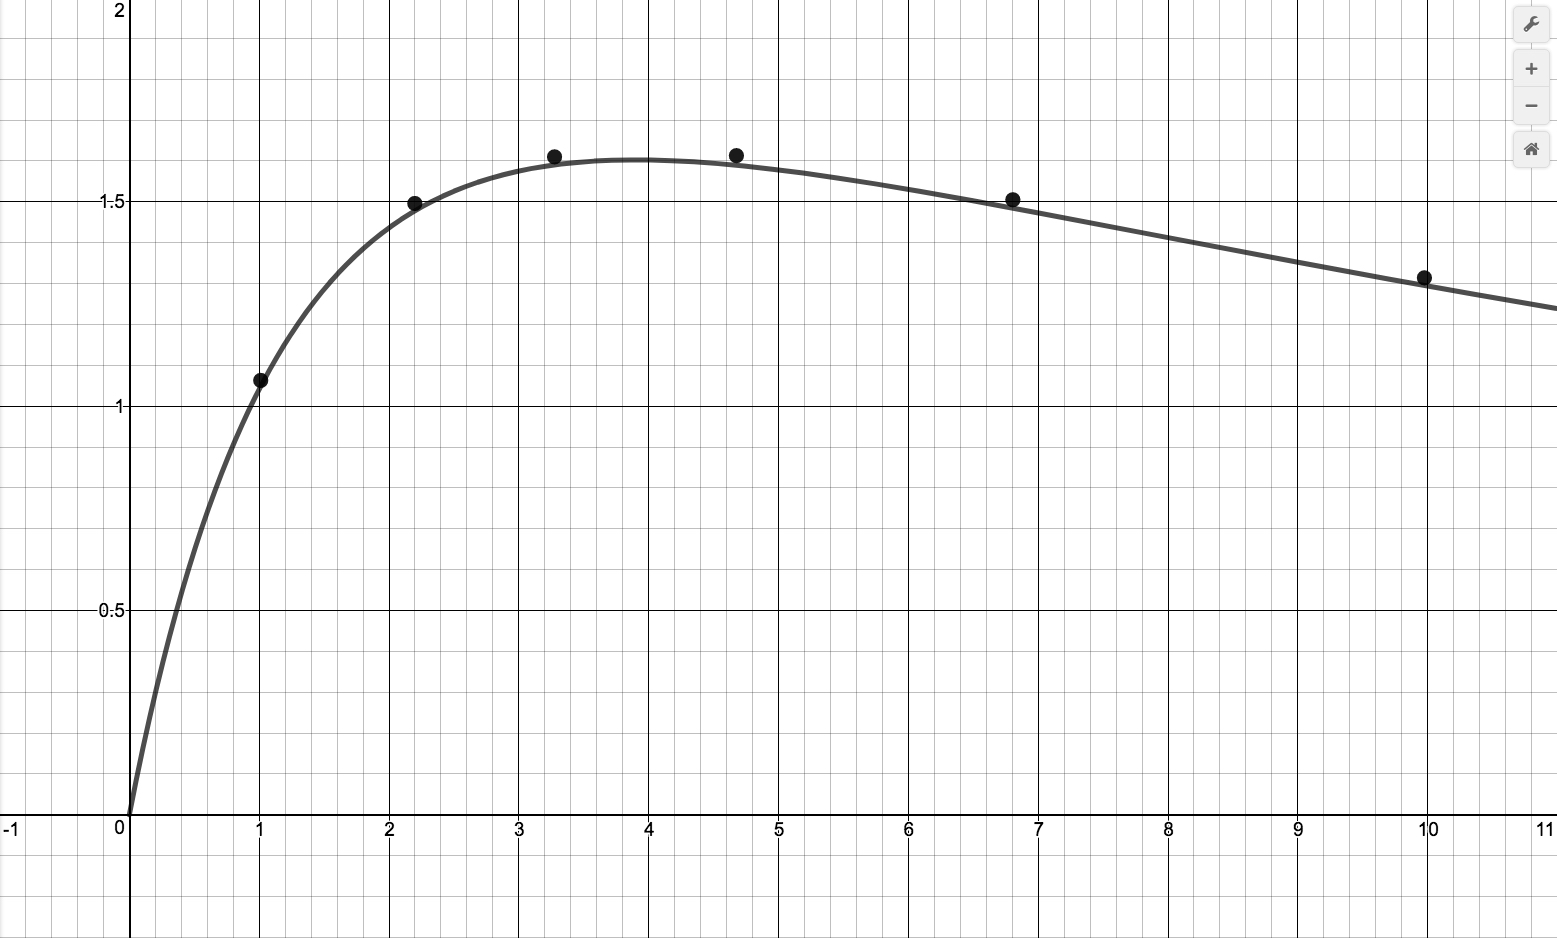
\includegraphics[height=2in]{./IntroRationalGraphics/MaxPowerRegression.jpg}

\item The maximum power is approximately $1.603 \; mW$ which corresponds to $3.9 \; k\Omega$.

\item As $x \rightarrow \infty, \; P(x) \rightarrow 0^{+}$ which means as the resistance increases without bound, the power diminishes to zero.

\end{enumerate}

\item  $a = -2$ and $c = -18$ so $f(x) = \dfrac{-2x^2+18}{x+3}$.

\item  \begin{multicols}{2}

 \begin{enumerate}

\item   $a=6$ and $n=2$ so $f(x) = \dfrac{6x^{2} -4}{2x^2+1}$

\item  $a=10$ and $n = 3$ so $f(x) = \dfrac{10x^{3} -4}{2x^2+1}$ .

\end{enumerate}
\end{multicols}


\item  If we define $f(x) = p(x) - p(a)$ then $f$ is a polynomial function with $f(a) = p(a) - p(a) = 0$.  The Factor Theorem guarantees $(x-a)$ is a factor of $f(x)$, that is, $f(x) = p(x) - p(a) = (x-a)q(x)$ for some polynomial $q(x)$. Hence, $r(x) = \frac{p(x)-p(a)}{x-a} = \frac{(x-a)q(x)}{x-a} = q(x)$ so the graph of $y = r(x)$ is the same as the graph of the polynomial $y = q(x)$ except for a hole when $x = a$.

\item  The slope of the curves near $x=1$ matches the exponent on $x$.  This exactly what we saw in  Exercise \ref{monomialarcexercise} in Section \ref{GraphsofPolynomials}.

\[ \begin{array}{|r||c|c|c|c|}  \hline

 f(x) &  [0.9, 1.1] & [0.99, 1.01] &[0.999, 1.001] & [0.9999, 1.0001]  \\ \hline
 x^{-1} & -1.0101 & -1.0001 & \approx -1 & \approx -1  \\  \hline
 x^{-2}& -2.0406& -2.0004 & \approx -2 & \approx -2   \\  \hline
 x^{-3} &-3.1021 & -3.0010 & \approx -3 & \approx -3   \\  \hline
 x^{-4} &-4.2057 & -4.0020 &\approx -4 & \approx -4   \\   \hline


\end{array} \]

\end{enumerate} 

\end{document}


\closegraphsfile